\documentclass[10.5pt, twocolumn]{article}

\usepackage[english]{babel}
\usepackage{graphicx}
\usepackage{imakeidx}
\usepackage{mathrsfs, amsmath}
\usepackage{systeme}
\usepackage{array}
\usepackage[utf8]{inputenc}
\usepackage{siunitx}
\usepackage{booktabs}
\usepackage{adjustbox}
\usepackage{geometry}
\geometry{a4paper,total={145mm,210mm}}
\usepackage{makecell}
\usepackage{afterpage}
\usepackage{listings}
\usepackage{subcaption}
\usepackage[toc,page]{appendix}
\usepackage[table]{xcolor}
\usepackage{pifont} % ding symbols
\usepackage{tikz}
\usepackage{changepage}
\usepackage{multirow} % multi row in tables
\usepackage{booktabs}
\usepackage{textcomp} % registered and copyright symbol
\usepackage{lscape} % vertical instead to horizontal
\usepackage{longtable} % for more page tables
\usepackage{eurosym}
\usepackage{lmodern}
\usepackage{amstext}
\usepackage{pdfpages} % import pdf pages
%\usepackage[hidelinks]{hyperref} % delete ugly hyperref borders of hyperlink
\usepackage{hyperref} % internal hyperlinks
\usepackage{titling} % titles
\usepackage{titlesec} % subtitles
\usepackage{blindtext} % for casual texts
\usepackage{dblfloatfix} % forces image at bottom in two-column files
\usepackage{gensymb} % standard unit of measurement
\usepackage{enumitem}

\DeclareRobustCommand{\officialeuro}{%
  \ifmmode\expandafter\text\fi
  {\fontencoding{U}\fontfamily{eurosym}\selectfont e}}



\makeindex[columns=2, title=Indice alfabetico, options= -s mystyle.ist, intoc]

\newcommand*{\Scale}[2][4]{\scalebox{#1}{\ensuremath{#2}}}
\renewcommand*\contentsname{Indice}
\newcommand*\NewPage{\newpage\null\thispagestyle{empty}\newpage}
\newcommand{\Virgolette}[1]{``#1''}
\newcommand*\circled[1]{\tikz[baseline=(char.base)]{
  \node[shape=circle,draw,inner sep=2pt] (char) {#1};}}
\newcommand{\tikzcircle}[2][red,fill=red]{\tikz[baseline=-0.5ex]\draw[#1,radius=#2] (0,0) circle ;}%command for draw text circle coloured
\def\changemargin#1#2{\list{}{\rightmargin#2\leftmargin#1}\item[]}
\let\endchangemargin=\endlist
\makeatletter
\let\originalpart=\part



\newcolumntype{C}[1]{>{\centering\arraybackslash}p{#1}}
\newcolumntype{L}[1]{>{\arraybackslash}p{#1}}
\newcolumntype{R}[1]{>{\raggedleft}p{#1}}
\newcolumntype{G}[1]{>{\centering\arraybackslash\columncolor{gray0}}p{#1}}

\definecolor{gray0}{gray}{0.9}
\definecolor{gray1}{gray}{0.7}
\definecolor{gray2}{gray}{0.4}

\lstset{
  literate = {α}{{$\alpha$}}1 {∆}{{$\Delta$}}1 {θ}{{$\theta$}}1 {η}{{$\eta$}}1 {→}{{$\rightarrow$}}1 {∂}{{$\partial$}}1, %tutti i simboli da usare come codice
  language = Mathematica % linguaggio
}
\hypersetup{
  citebordercolor=red
}


% ----- TITLE
\titleformat*{\section}{\Large\bfseries}
\title{
  \large{University of Trento}\\
  \normalsize{Master in Mechatronics Engineering}\\
  \vspace{0.2cm}
  \large{\textit{Modelling and Simulation of Mechatronics Systems}}\\
  \vspace{0.2cm}
  \Large{\textbf{Development, analysis and optimization of the performance of an innovative driving simulator}}\\
  \vspace{0.25cm}
  \hrule
  \vspace{0.2cm}
  \large{\textbf{Kinematics analysis}}\\  % Title
  \vspace{0.2cm}
  \hrule
}
\author{A. Comoretto \and J. Losi \and S. Valentini}
\date{\vspace{0.5cm}}
% ----- TITLE


\begin{document}
\maketitle
The kinematics analysis of the system is crucial in the modelling process of the driving simulator mechanism.

First, the position analysis is carried out, with the objectives of obtaining the workspace of the mechanism and the inverse solution.

Second, the velocity analysis is developed, obtaining the velocity ratios between the platform variables and the linear actuators as function of the position of the actuators themselves. Moreover, the linear and angular velocities of the plaftorm is obtained as function of each linear actuators position, keeping the other two at unitary velocity.

Third, the acceleration analysis has been carried out similarly to the velocity, by keeping two actuators at unitary acceleration.

Finally, a possible direction for an optimization method is proposed, exploring the effect of the various design parameters on the workspaces.

\section{Position analysis}
\label{s:Position}
In this section the mechanism's behaviour is studied.
In Figure \ref{f:Top-View} is shown the top view of the mechanism.
\begin{figure}[h!]
  \centering
  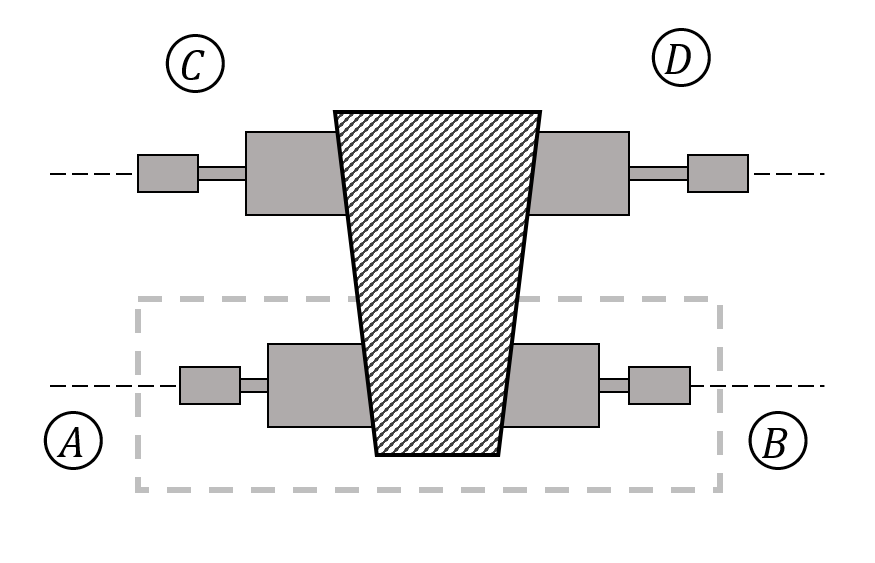
\includegraphics[width=7cm]{Images/Mechanism_TopView}
  \caption{Top view of the full-mechanism.}
  \label{f:Top-View}
\end{figure}

In first approximation a 2D analysis is conduced, and is refered only to the bodies \circled{A} and \circled{B}. This simplification allows to focus only on three degrees of freedom (DoFs) of the driving simulator: Sway, Heave, Roll. Future analysis involving also the sub-systems \circled{C} and \circled{D} would allow considerations on the other DoFs.
\begin{figure*}[h!]
  \centering
  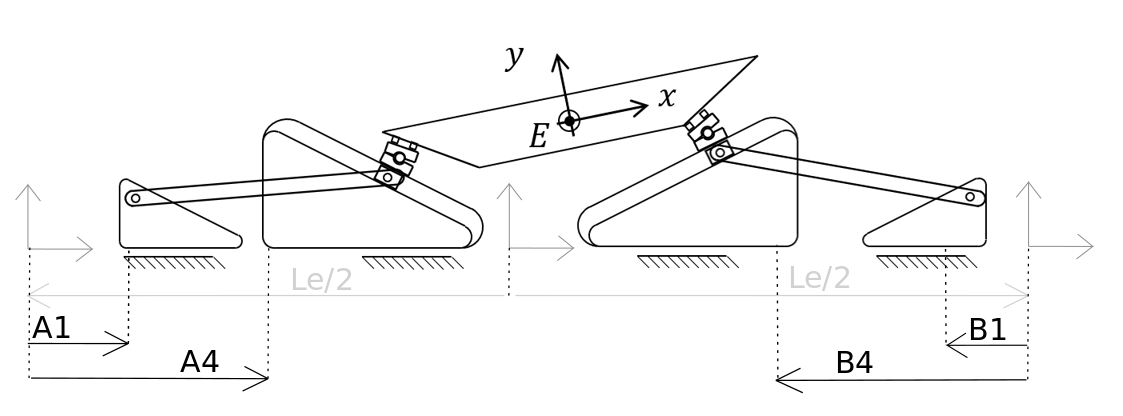
\includegraphics[width=12cm]{Images/Mechanism_LateralView_better}
  \caption{2D mechanism.}
  \label{f:2D_Mechanism}
\end{figure*}
\subsection{Direct position analysis}
\label{s:Direct-position}
The mechanism studied in the 2D simplification is the marked part in Figure \ref{f:Top-View}, in fact only sub-mechanisms \circled{A} and \circled{B} are taken into account. The studied mechanism is shown in Figure \ref{f:2D_Mechanism}.

For the 2D analysis it is chosen to consider the length of the platform as a constant, even if it could be variable, due to its geometry. The variability of the length of the platform would introduce another DoF orthogonal to the plane, not described properly by this model. Only in future works on the 3D model this fact should be taken into account.

The full 2D mechanism is composed by two mirrored sub-mechanisms, made by four sub-bodies, joined by the platform, as shown in Figure \ref{f:2D-Mechanism}. Each sub-mechanism can be described as shown in Figure \ref{f:Sub-Mechanism}.
\begin{figure*}[h!]
  \centering
  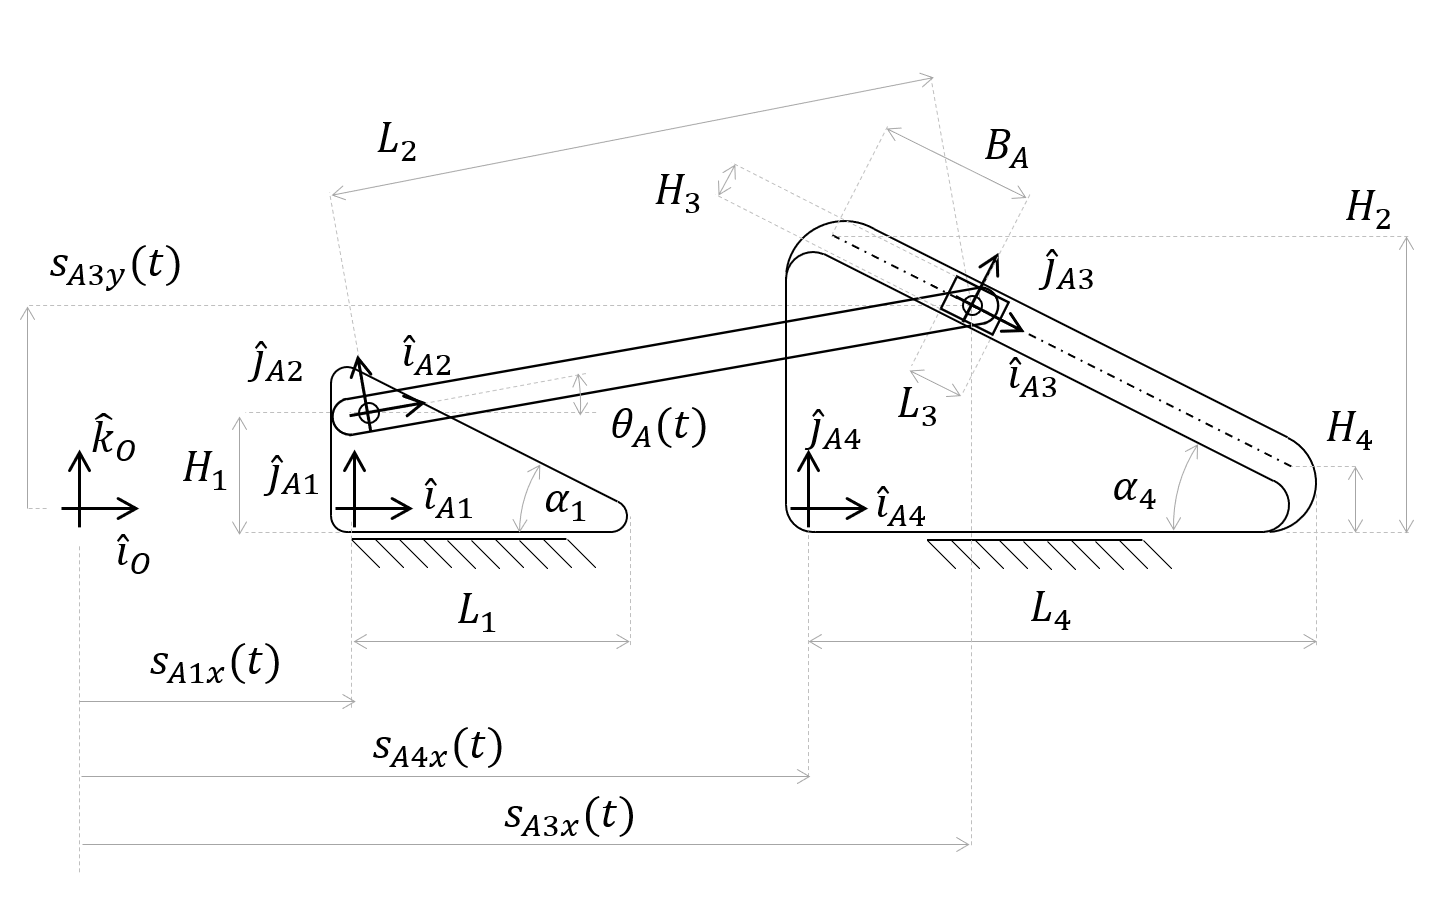
\includegraphics[width=12cm]{Images/Sub-Mechanism}
  \caption{One of the four sub-mechanism of the structure.}
  \label{f:Sub-Mechanism}
\end{figure*}
Note that the same model can be developed for all the other sub-mechanisms by changing the subscripts.
The actuators' variables are computed starting from two auxiliary reference frames (RF), one located to the left and one to the right of the fixed central RF by a distance equal to \(L_e/2\).\\
At a first sight, it could be natural to say that the four motors could be independant variables:
\begin{itemize}
  \item \( s_{A1x}(t) \);
  \item \( s_{A4x}(t) \);
  \item \( s_{B1x}(t) \);
  \item \( s_{B4x}(t) \).
\end{itemize}
Although the apparent simplicity of this consideration, it doesn't match with the previous one: in fact considering the length of the platform (named \( L_5\)) constant means that one of the motor has to be considered as a dependant variable.

In particular \( s_{B1x}(t) \) is considered the dependant variable, while the other three actuators consitute the independent variables set \( q_{I} \).

At the same time it has to be defined a set of dependant variables \( q_{D} \).
In particular for the description of the sub-mechanism's behaviour the following elements are chosen:
\begin{itemize}
  \item \( s_{A3x}(t) \) and \( s_{A3y}(t) \) which are the space coordinates of the body 3;
  \item \( \theta_A(t) \) which is the angle of the body 2;
  \item \( B_A(t) \) which is the distance of the body 3 from the upper-left edge of the body 4.
\end{itemize}
To write the kinematics equations, the chosen approach involves a combination of the recursive and global approaches.\\
The mechanism is treated as the combination of two sub-systems \circled{A} and \circled{B}, each one them representing a closed loop from the kinematics point of view, solved using two recursive chains constrained at the inclined runner (body 3). Then, the last constraint equation is built up imposing that the platform links the two sub-systems.\\
This approach is particularly powerful, considering the simple symbolic expression that results from the inverse analysis carried on in Section \ref{s:Inverse-position}.

Solving the system of 6 constraints equations in 9 variables leads to a symbolic expression of the 6 dependent variables \( q_{D} \) as function of the actuators. The expression of the pose of the center of mass of the platform, treated as end effector (EE) of the system, is derived from \( q_{D} \) by exploiting simple geometic considerations.

It's important to underline that the same procedure can be followed choosing \( s_{A1x}(t) \) instead of \( s_{B1x}(t) \) as powered off actuator, i.e. dependent variable. All the results showed in the next sections would be mirrored, due to the geometrical symmetry of the system.

The results of this section are essential for the computation of the admittable extremes for the actuators, done in \ref{s:Extreme-positions}, and for the definition of the workspaces of the 2D-system, carried out in Section \ref{s:Position-workspaces}.

\subsection{Initial position problem}
\label{s:Initial-position}
The following is a simple criterion, based on geometrical considerations, for the determination of the initial values to be assigned to the actuators. The initial position is defined as follows:
\begin{equation}
  s_{A1x,0} = 0
\end{equation}
\begin{equation}
  s_{A4x,0} = \sqrt{L_2^2-\frac{H_2+H_4-2H_1}{4}} - \frac{L_4}{2}
\end{equation}
and the symmetrical happens for the fixed position for the sub-mechanism \circled{B} (\( s_{A1x,0} = s_{B1x,0} \) and \( s_{A4x,0} = s_{B4x,0} \)).

The complete formulation of the initial position involves also the definition of the distance \( L_e \) between left and right auxiliary RF and the fixed RF:
\begin{multline}
  L_e = 2*\sqrt{L_2^2-(\frac{H_2-H_4}{2}-H1+H4)^2}+\\
  + Q_3*\sin(\alpha_4)) + L_5
\end{multline}
that depends on the length of the platform \( L_5 \). Since the length of the platform, as it can be seen in Figure \ref{f:Top-View}, in general is variable from two values \cite{aVDS}, the initial position problem depends on it.

\subsection{Extreme positions problem}
\label{s:Extreme-positions}
A crucial part of the analysis deals with the definition of an automated way to determine the maximum range of variability of one actuator, say actuator 4 of \circled{B}, given any values of the other two. In general one could exploit the velocity analysis and determining the points at which the velocity ratios goes to infinity. Unfortunately this method is not effective, since inside these extremes there are configurations that imply compenetration of bodies.

Said so, a develpment of a consistent approach for the determination of the possible ranges of the actuators is considered necessary.\\
The developed criterion considers that:
\begin{itemize}
  \item the maximum and minimum position of the inclined runner through its seat is limited by limit switches positioned at an height of \( H_2 \) and \( H_4 \) respectively;
  \item the body 1 of each sub-system should not interpenetrate the body 4;
  \item the two bodies 4 of sub-systems \circled{A} and \circled{B}, i.e. the bodies below the platform, should not interpenetrate themselves.
\end{itemize}
The constraints are here summarized:
\begin{equation}
    s_{A1}x(t)+L_1 < s_{A4x}(t)+c_0
\end{equation}
\begin{equation}
    H_4 < s_{A3y}(t)
\end{equation}
\begin{equation}
   s_{A3y}(t) < H_2
\end{equation}
\begin{multline}
    s_{A4x}(t) < s_{A1x}(t)+\\
    +L_2 \cdot cos(arctan(\frac{H_2-H_1}{L_2}))
\end{multline}
\begin{equation}
   s_{A4x}(t)+s_{B4x}(t)+2 L_4 < L_e-c_1
\end{equation}
The same is applied for sub-mechanism \circled{B}.
Two variables, useful for the optimization part, are also introduced:
\begin{itemize}
  \item \( c_0 \): accepted interpenetration between bodies 1 and 4;
  \item \( c_1 \): minimum distance required between the two sub-mechanisms \circled{A} and \circled{B}.
\end{itemize}

To perform this task in an automated way a Maple\textsuperscript{TM} function is written, \texttt{extremes(actuator, other\_actuators, data\_in, c0, c1)}, which returns a set containing the two lower and upper limits for \texttt{actuator} given \texttt{other\_actuators} representing the values of the other two.

\subsection{Position workspaces}
\label{s:Position-workspaces}
Following the approach introduced in the first paper \textit{\Virgolette{System requirements}}, in this section the three workspaces regarding the 2D-system are obtained. In particular, considering the 3 DoFs, they are:
\begin{itemize}
  \item workspace between Sway (\( x \)) and Heave (\( y \));
  \item workspace between Sway (\( x \)) and Roll (around \( z \));
  \item workspace between Heave (\( y \)) and Roll (around \( z \));
\end{itemize}

The objective is to build the workspaces exploiting a solid method, that could be useful in more advanced analysis, such as the one of Section \ref{s:Parameters}.

At first, \( x-y\) workspace is defined by moving only one actuator at time, while others are mantained fixed at their initial position. The range of variability of the activated actuator is defined by using \texttt{extremes} function described in \ref{s:Extreme-positions} and assigning the initial values to the other two.
Finally, by nesting this approach in three \texttt{for} loops, a cloud of points is obtained. Unfortunately, this approach is not effective, because for each \( (i j k) \)-th case in the loop, the admittable ranges for the actuators are always considered the same (computed at the initial position), and are not modified according to the new configuration.

This implies that the workspace is covering some points in which the geometrical constraints are violated. This can be easily proven using the solution (see Section \ref{s:Inverse-position}) of the inverse kinematics evaluated at any point near the boundary of the obtained workspace and observing that its representation shows a visible violation of such limits.

For this reason, an improved Maple\textsuperscript{TM} procedure has been developed. The main idea consists in continuously modifying the admittable range for the actuators on the base of the \( (i j k) \)-th iteration in the loop. This is realized forecasting, for each iteration cycle, the admittable ranges for each iteration. For example, the \( k \)'s admittable range is computed on the base of \( i \) and \( j \), and so on.

By doing so, an improved workspace has been obtained, true to the geometric constraints in each point. In Figures \ref{fig:clouds} and \ref{fig:proj_clouds} the two different approaches are compared, showing how the second gives a smaller area, where no compenetration of bodies is allowed.
\begin{figure}[h!]
	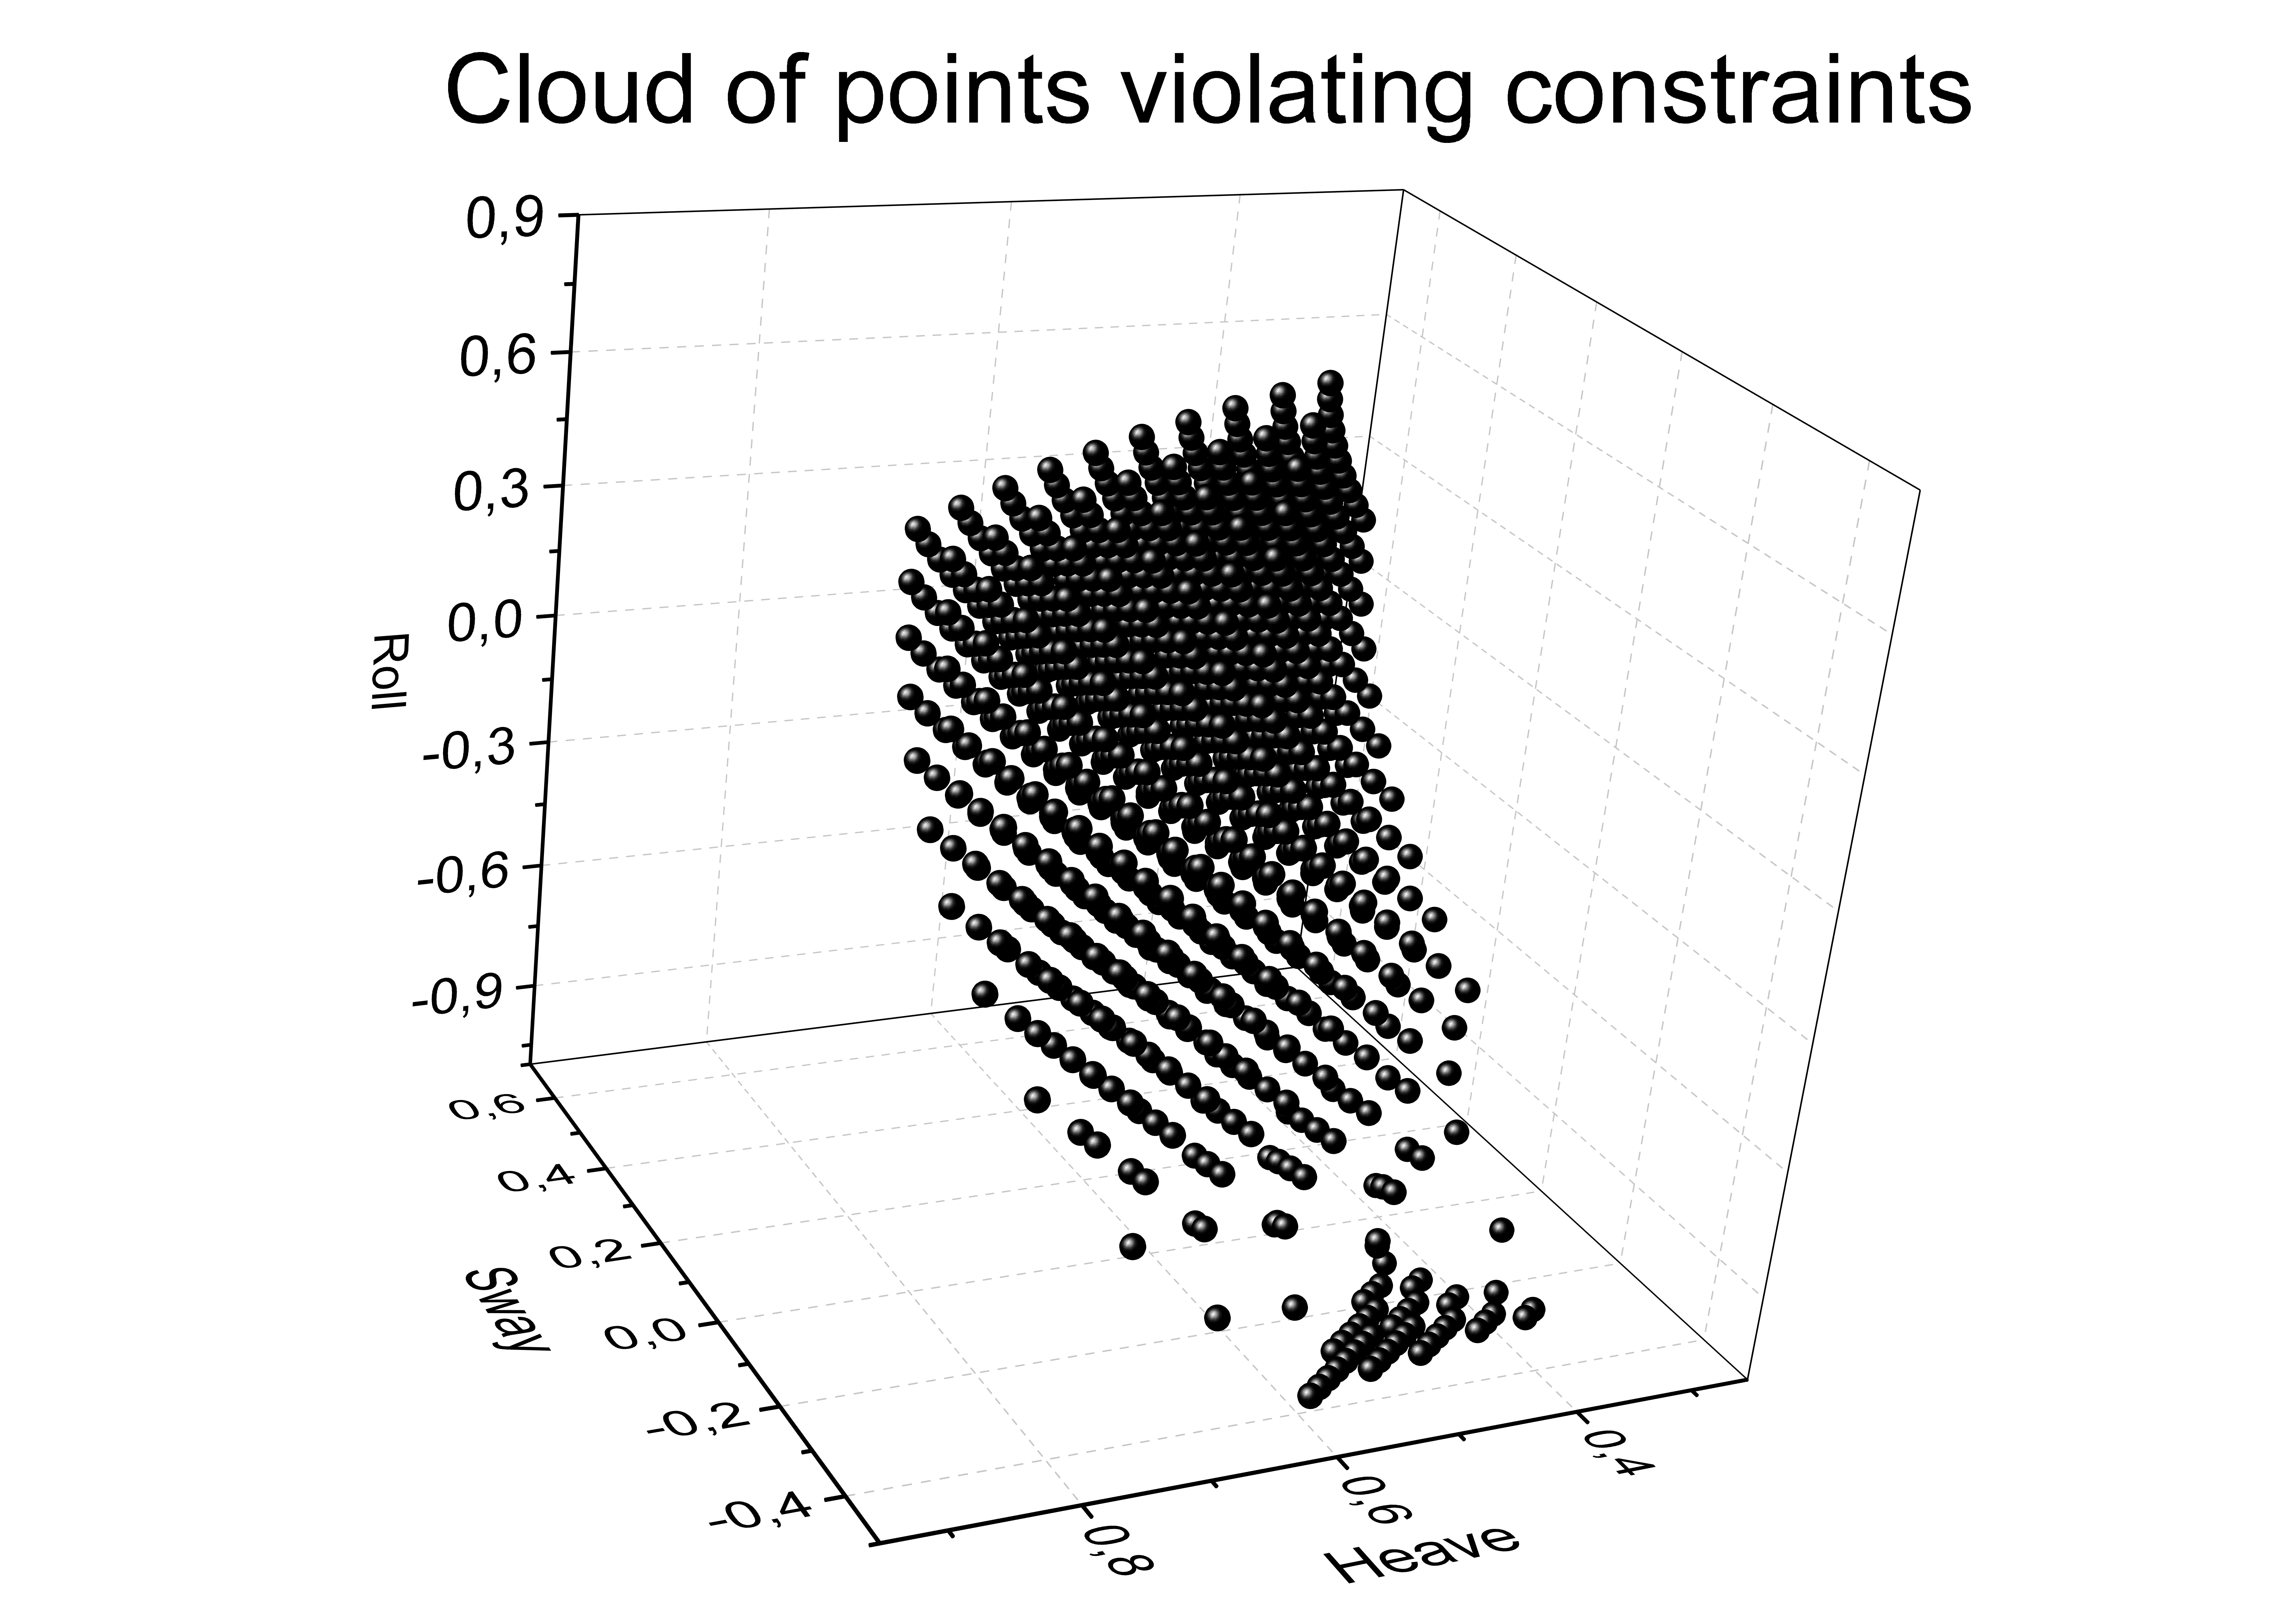
\includegraphics[width=7.5cm]{Images/CloudPoints_bad}
    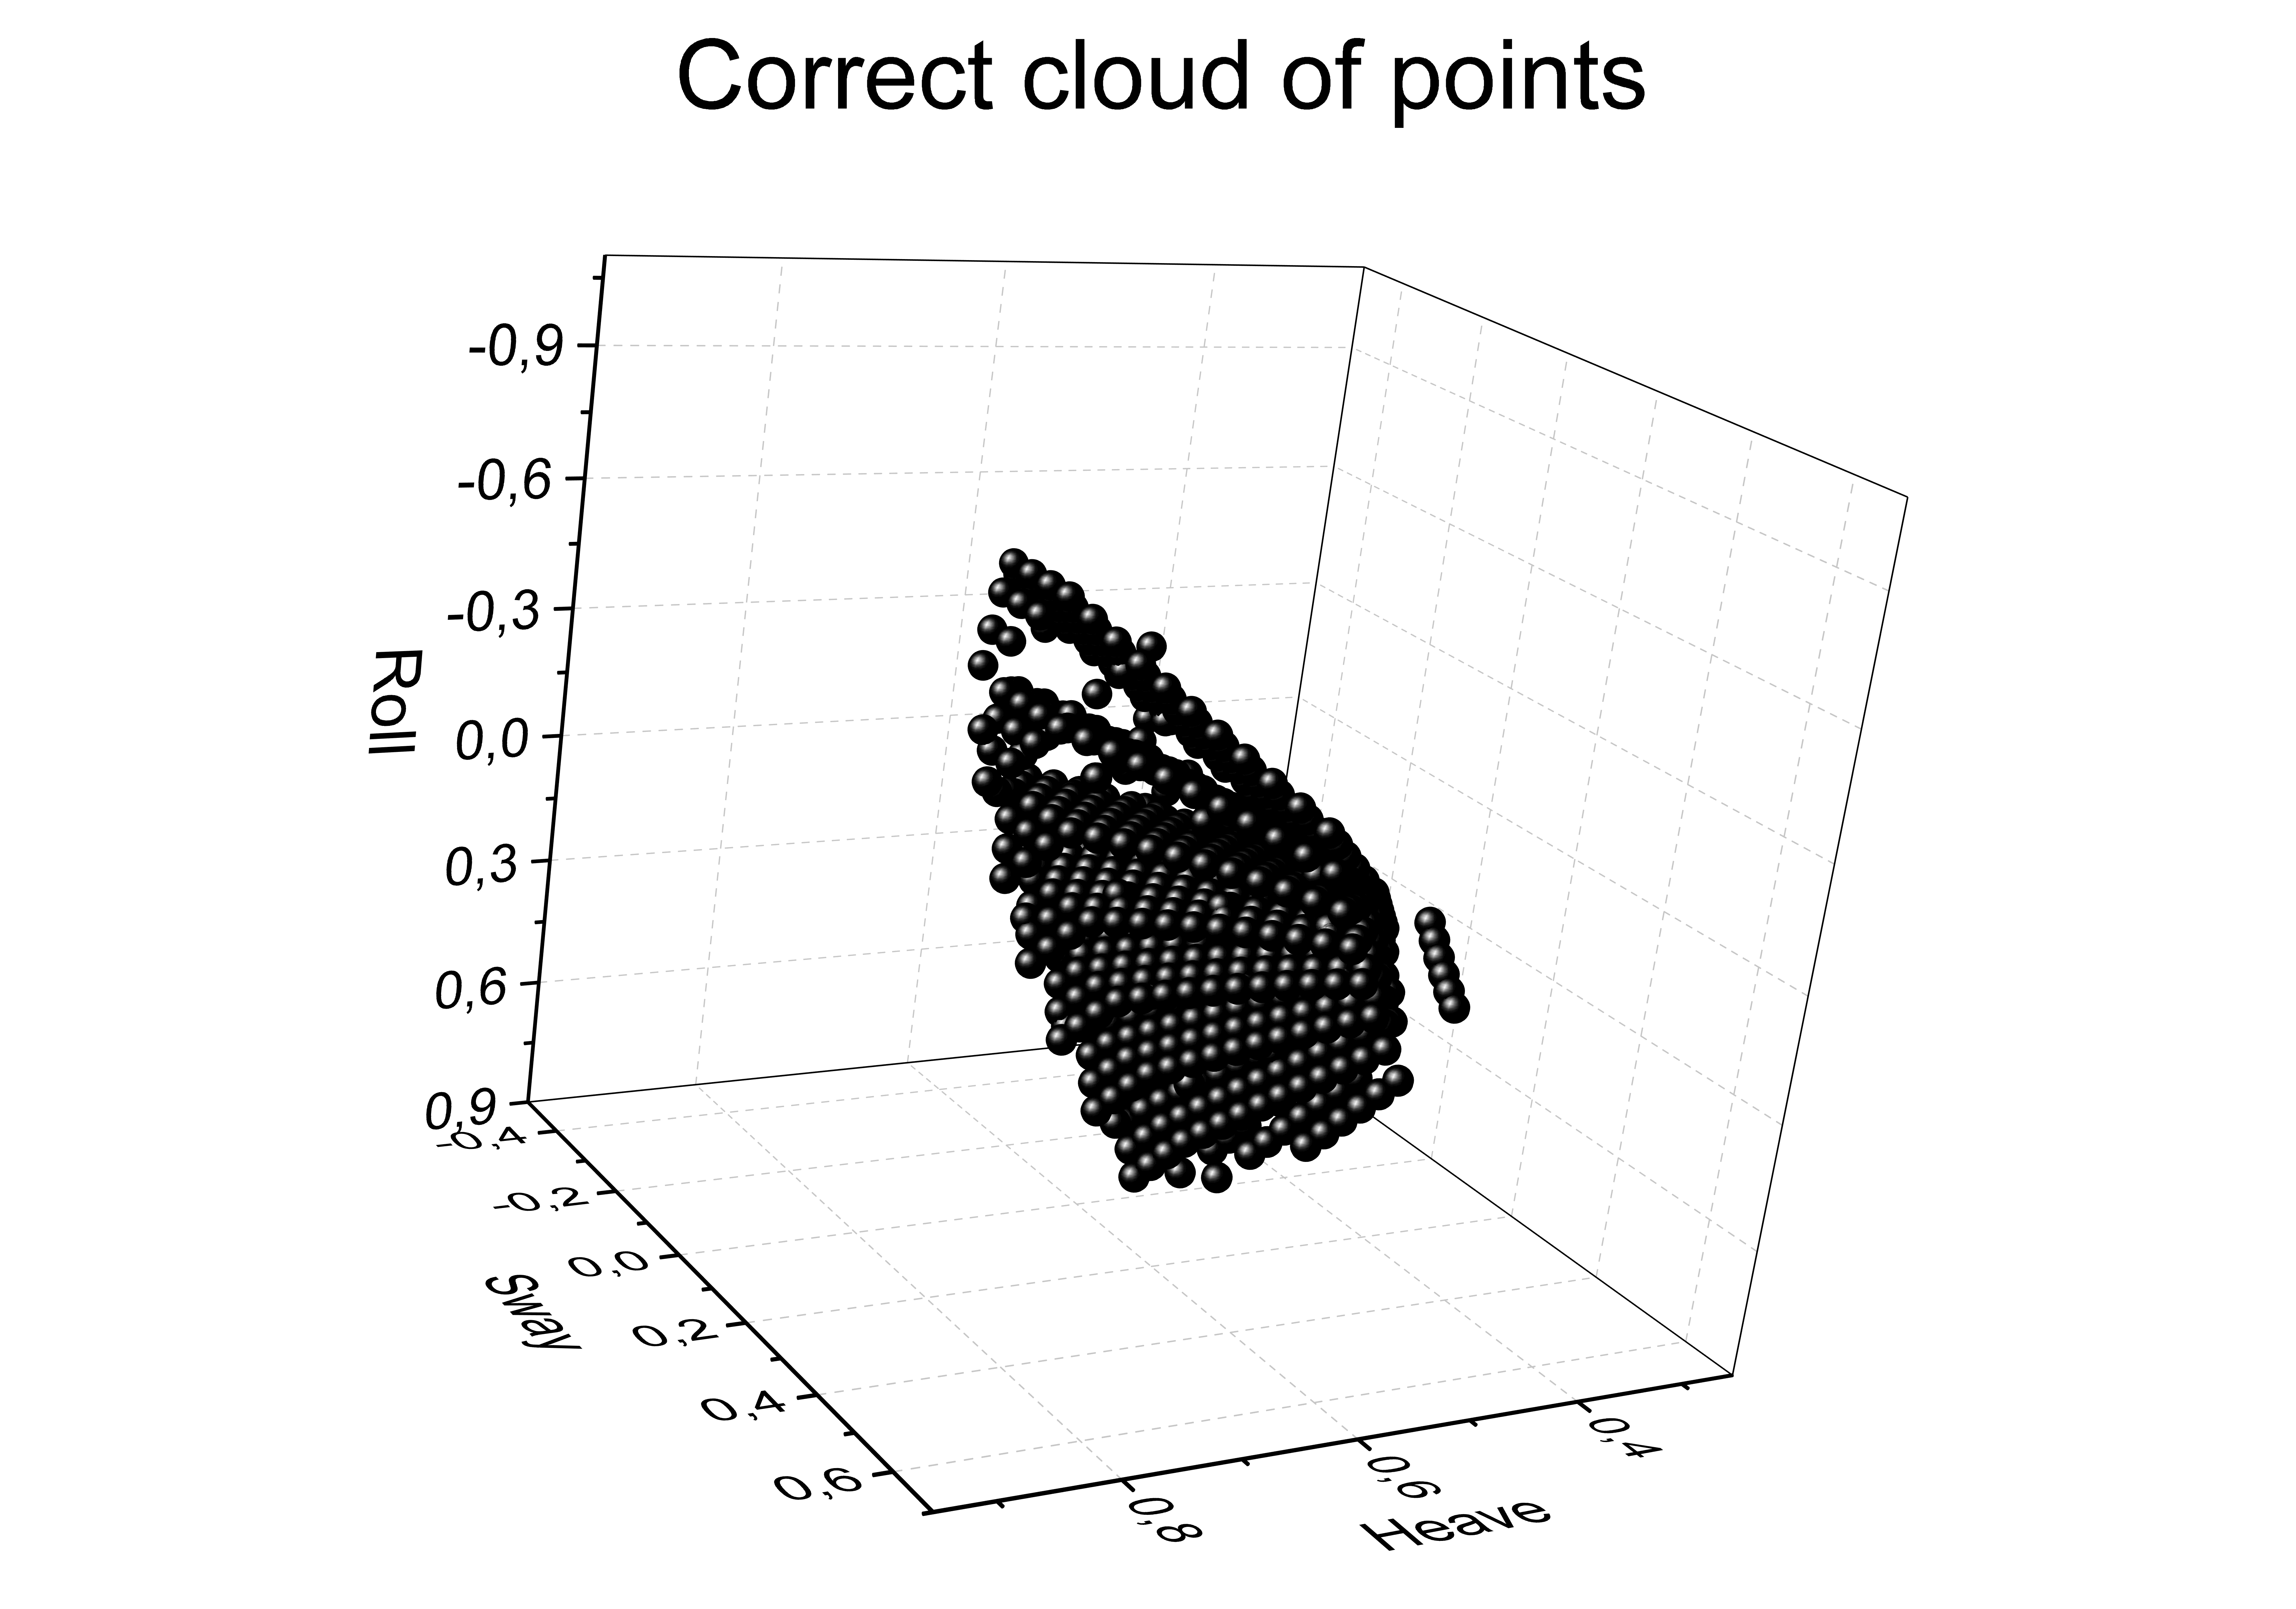
\includegraphics[width=7.5cm]{Images/CloudPoints_tot}
	\caption{The two obtained cloud of points: the first one must be discarded.}
  \label{fig:clouds}
\end{figure}
\begin{figure}[h!]
	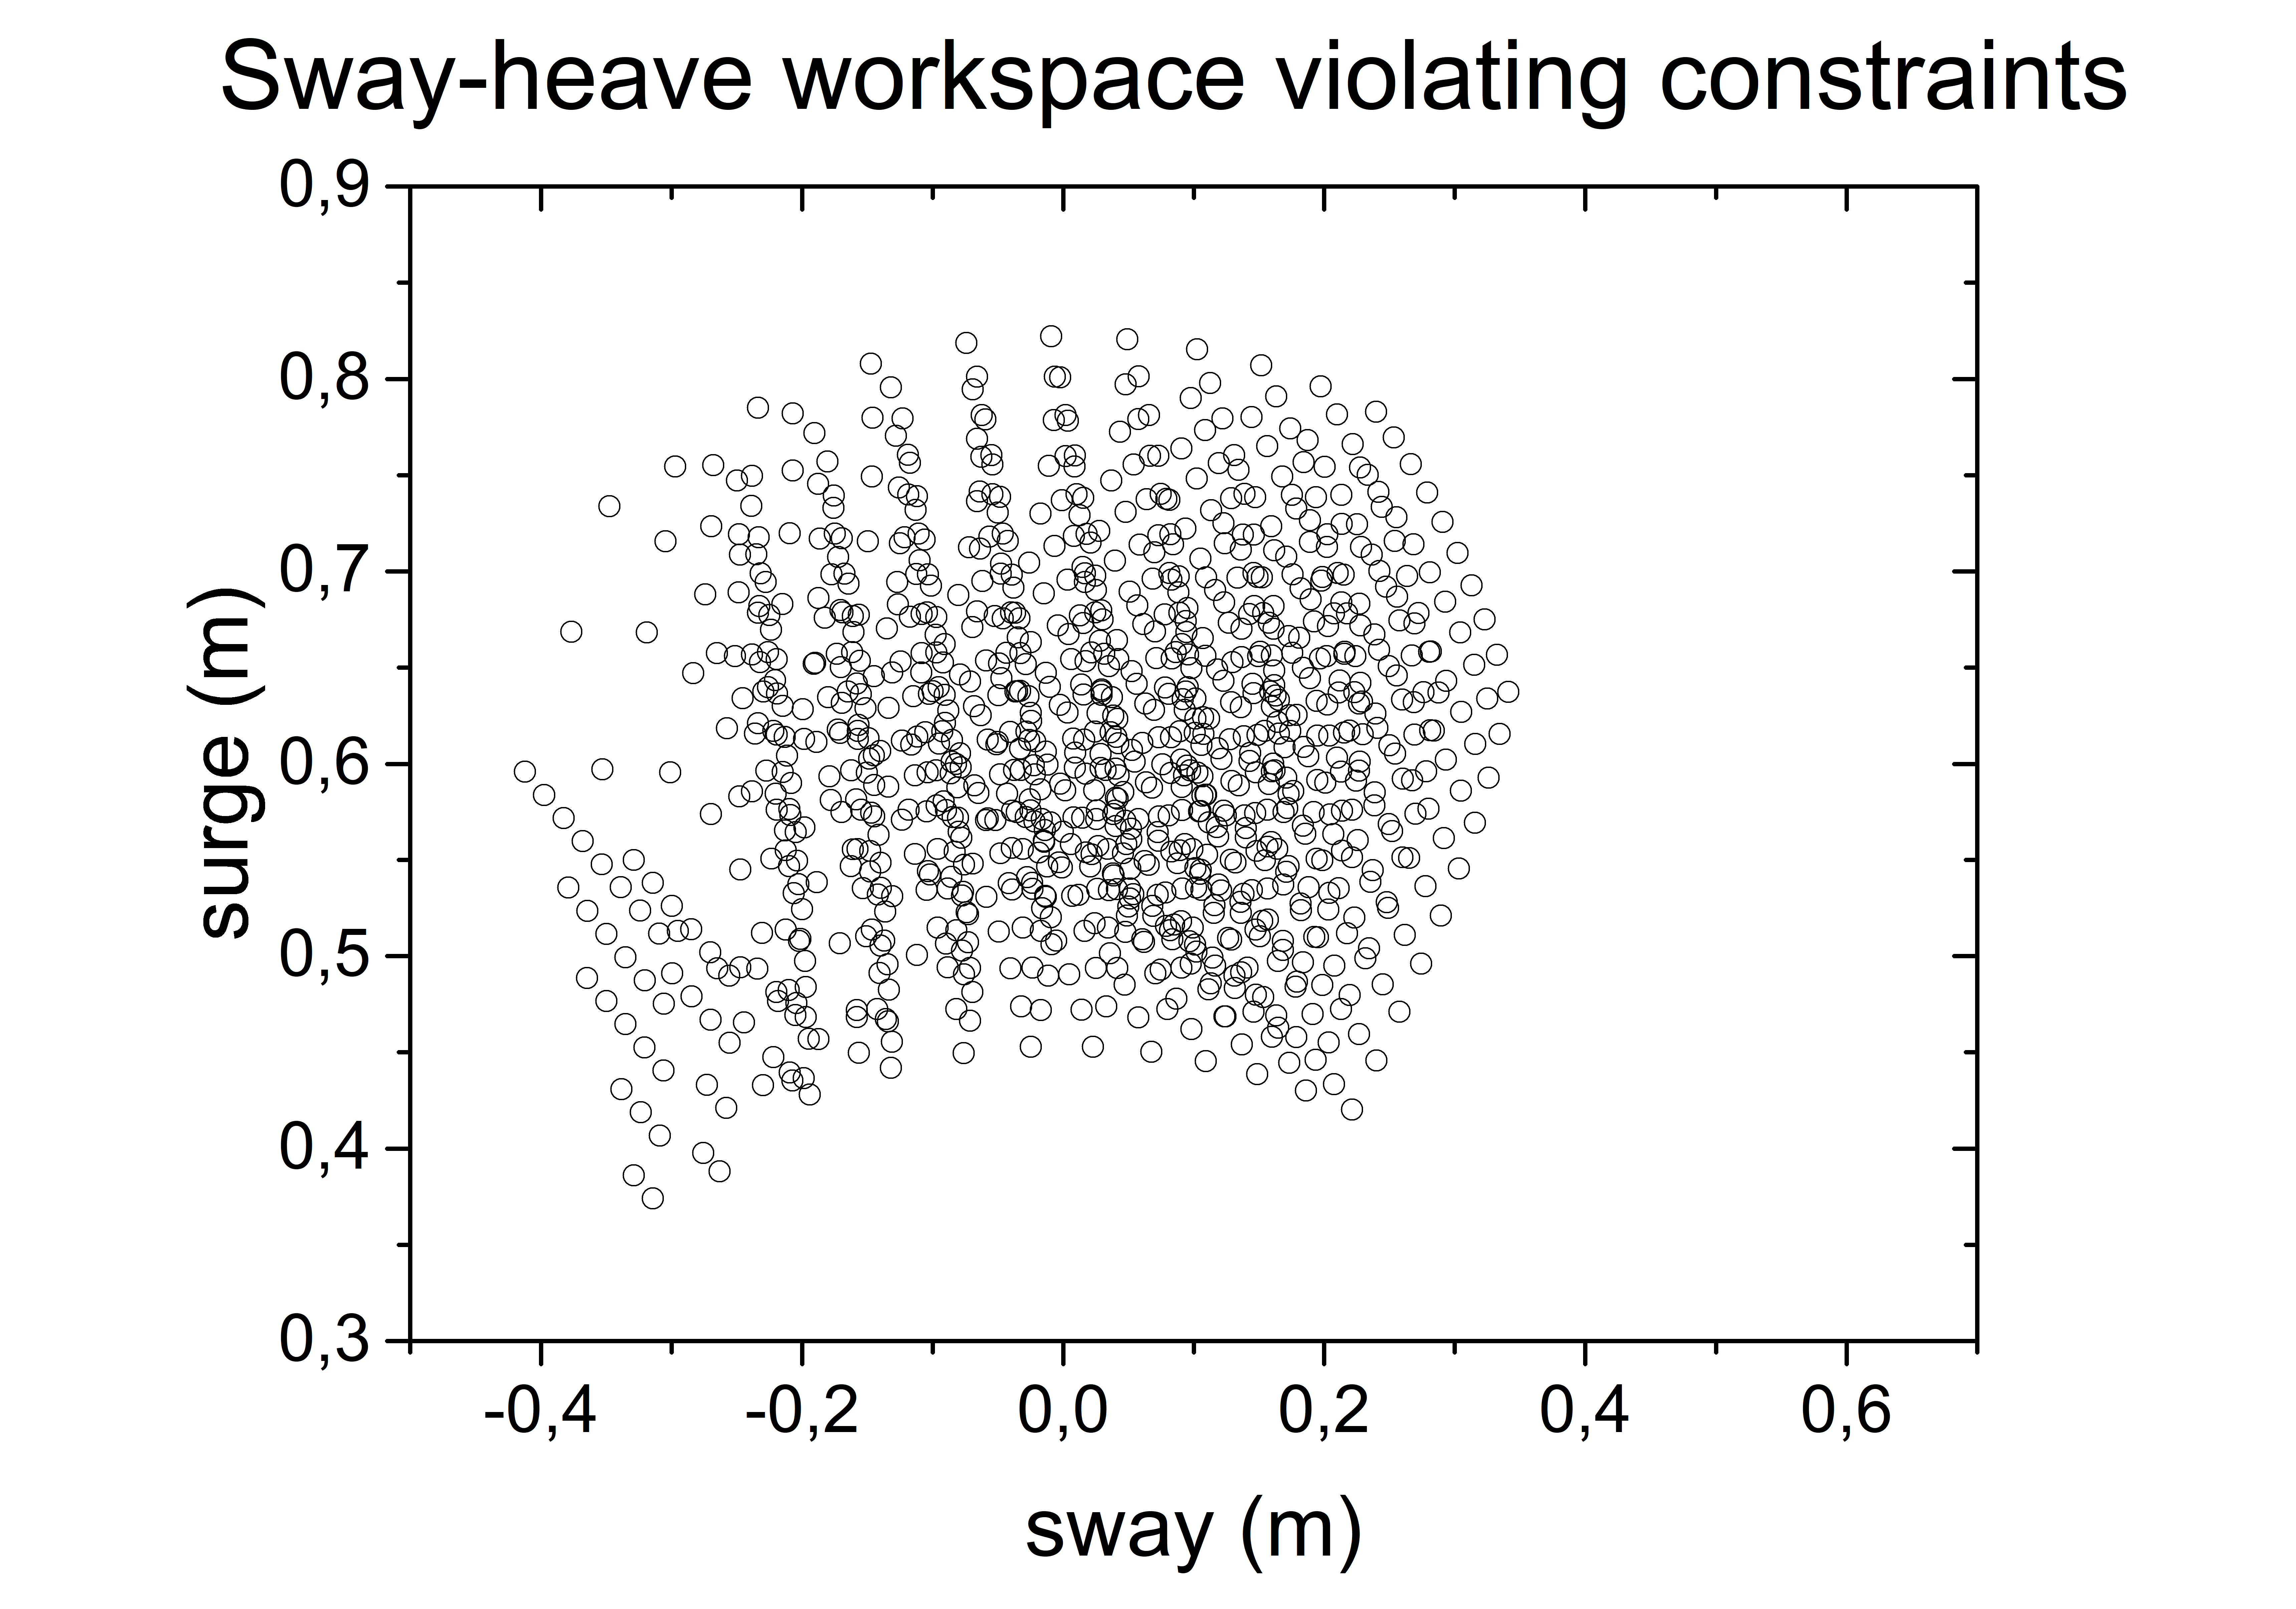
\includegraphics[width=7.5cm]{Images/ws_xy_bad}
    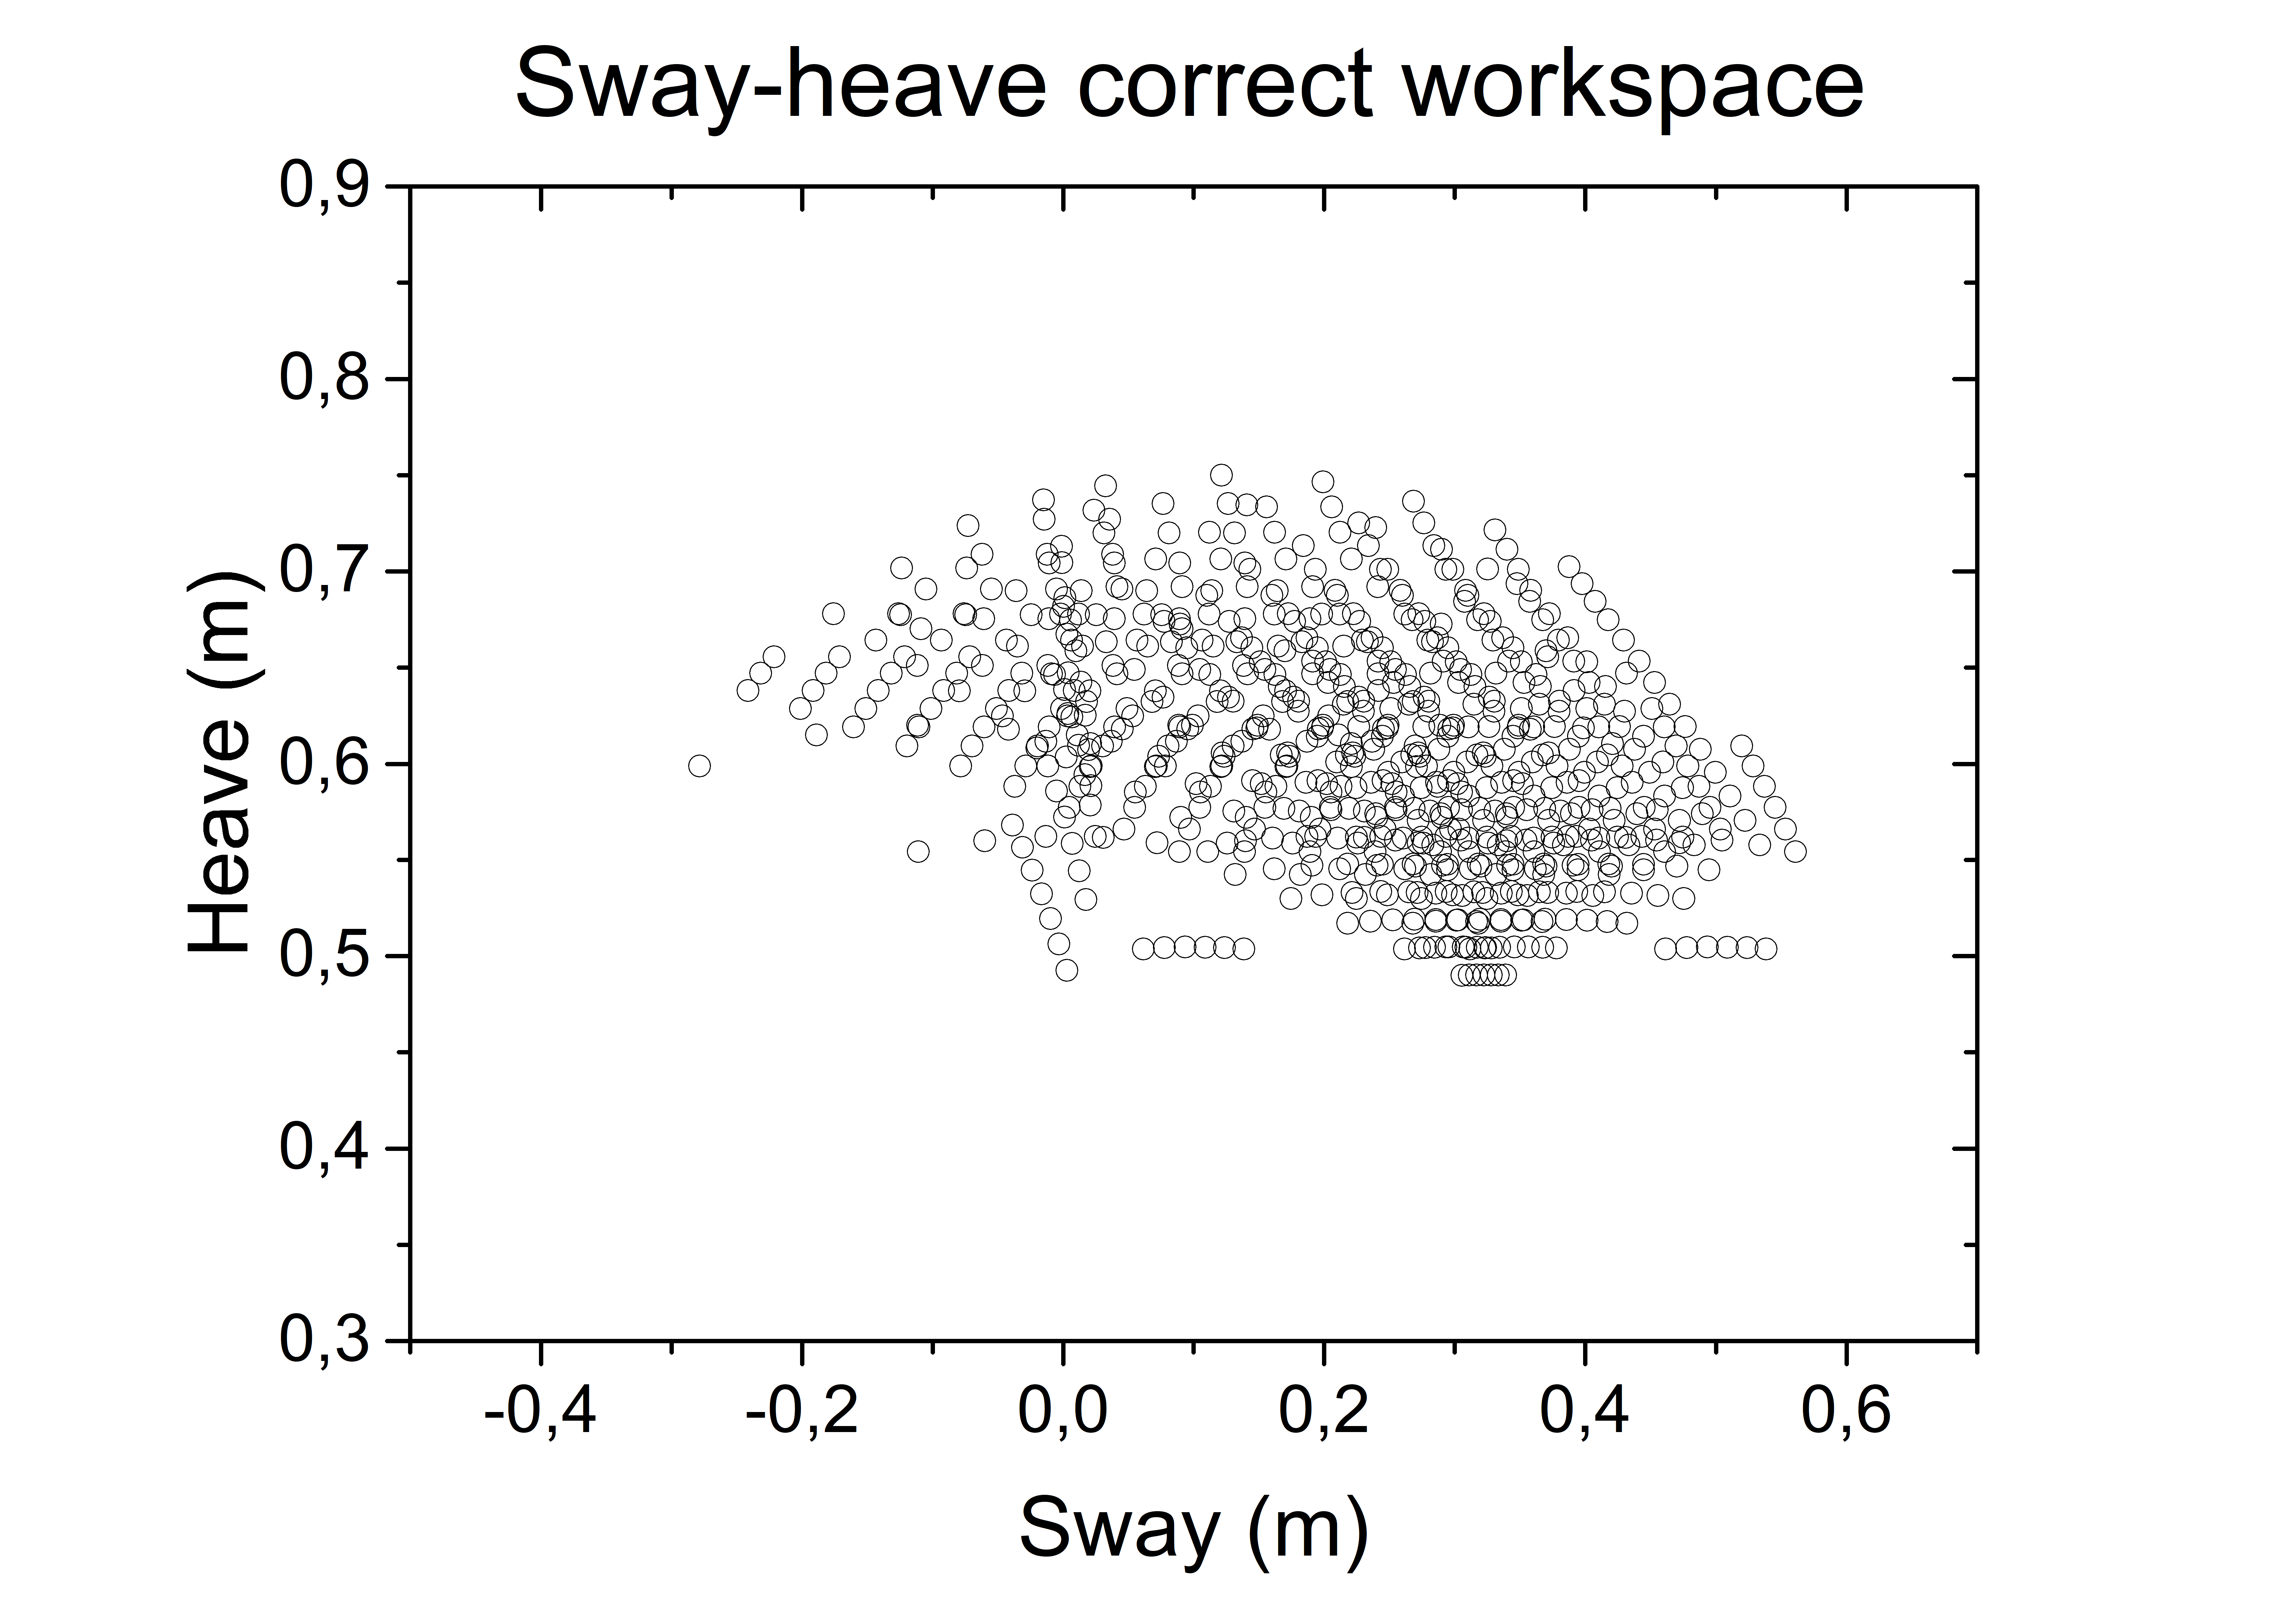
\includegraphics[width=7.5cm]{Images/ws_xy_tot}
	\caption{Projection over the \textit{sway}-\textit{heave} plane of the two clouds of points, the wrong one and the correct one.}
  \label{fig:proj_clouds}
\end{figure}

\subsection{Inverse position analysis}
\label{s:Inverse-position}
The direct position problem has been carried on in Section \ref{s:Direct-position}. The inverse problem, i.e. obtaining the values of the actuators that realize the desired pose of the platform's center fo mass, is explained in this section.

The original system of 6 constraints equations has been filled with the three equations describing the Sway, Heave and Roll of the platform. Then the actuators variables have been obtained, solving the system with the platform variables treated as independent.
This symbolic expression has been used to derive the values of the actuators that realize some target motions.

In particular, the target motion used as example is taken from the experimental data acquired in the first paper \textit{\Virgolette{System requirements}}. At any time, the pose of the platform center of mass is described by:
\begin{itemize}
  \item Sway and Heave fixed at initial condition;
  \item variable Roll, described by the trajectory in Figure \ref{fig:experimental}.
\end{itemize}

Applying the inverse kinematics solution at each time instant, the three values of the actuators are derived, as shown in Figure \ref{fig:experimental}.

An interesting information that can be derived by this result regards the necessary range for the actuators to operate. Unfortunately, in the case of the analyzed configuration, the procedure \texttt{extremes} mentioned in \ref{s:Extreme-positions} gives an interval which is not compatible with this motion. Further design steps should proceed towards the compatibility between the doable actuators intervals and the necessary ones, that come from the inverse kinematics applied at experimental data.

\begin{figure}[h!]
	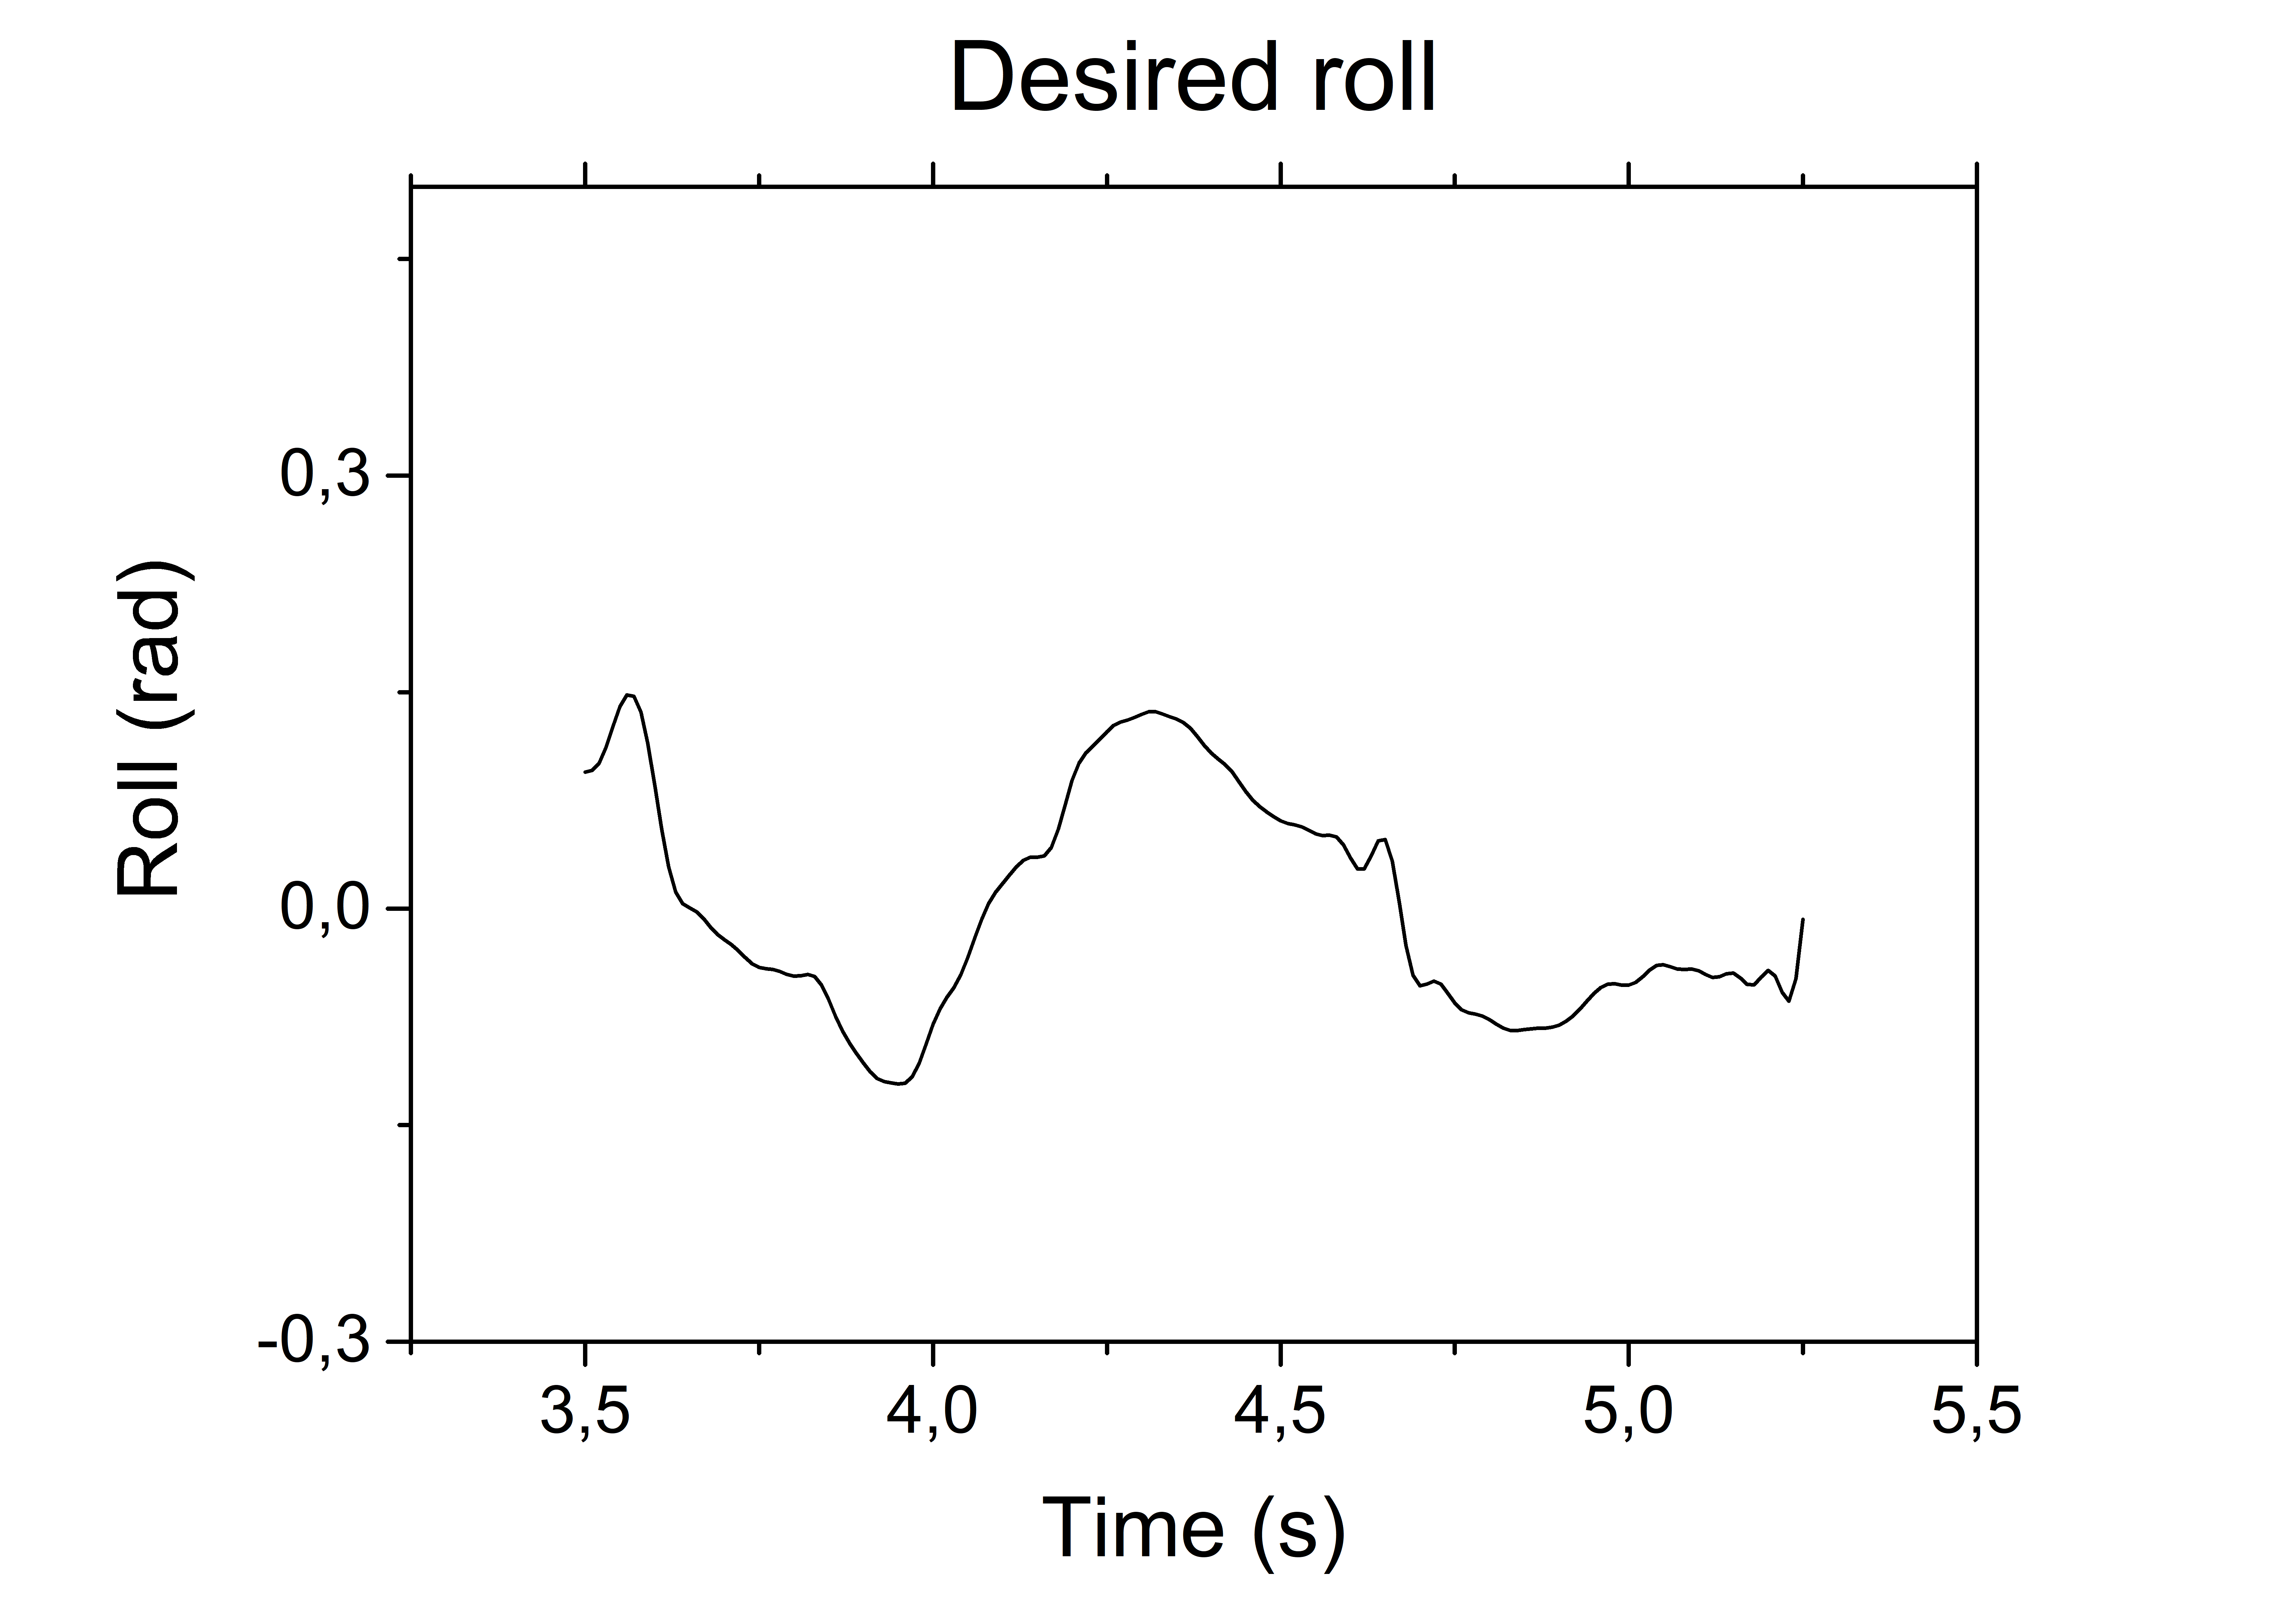
\includegraphics[width=7.5cm]{Images/RollDesired_InvKine}\\
    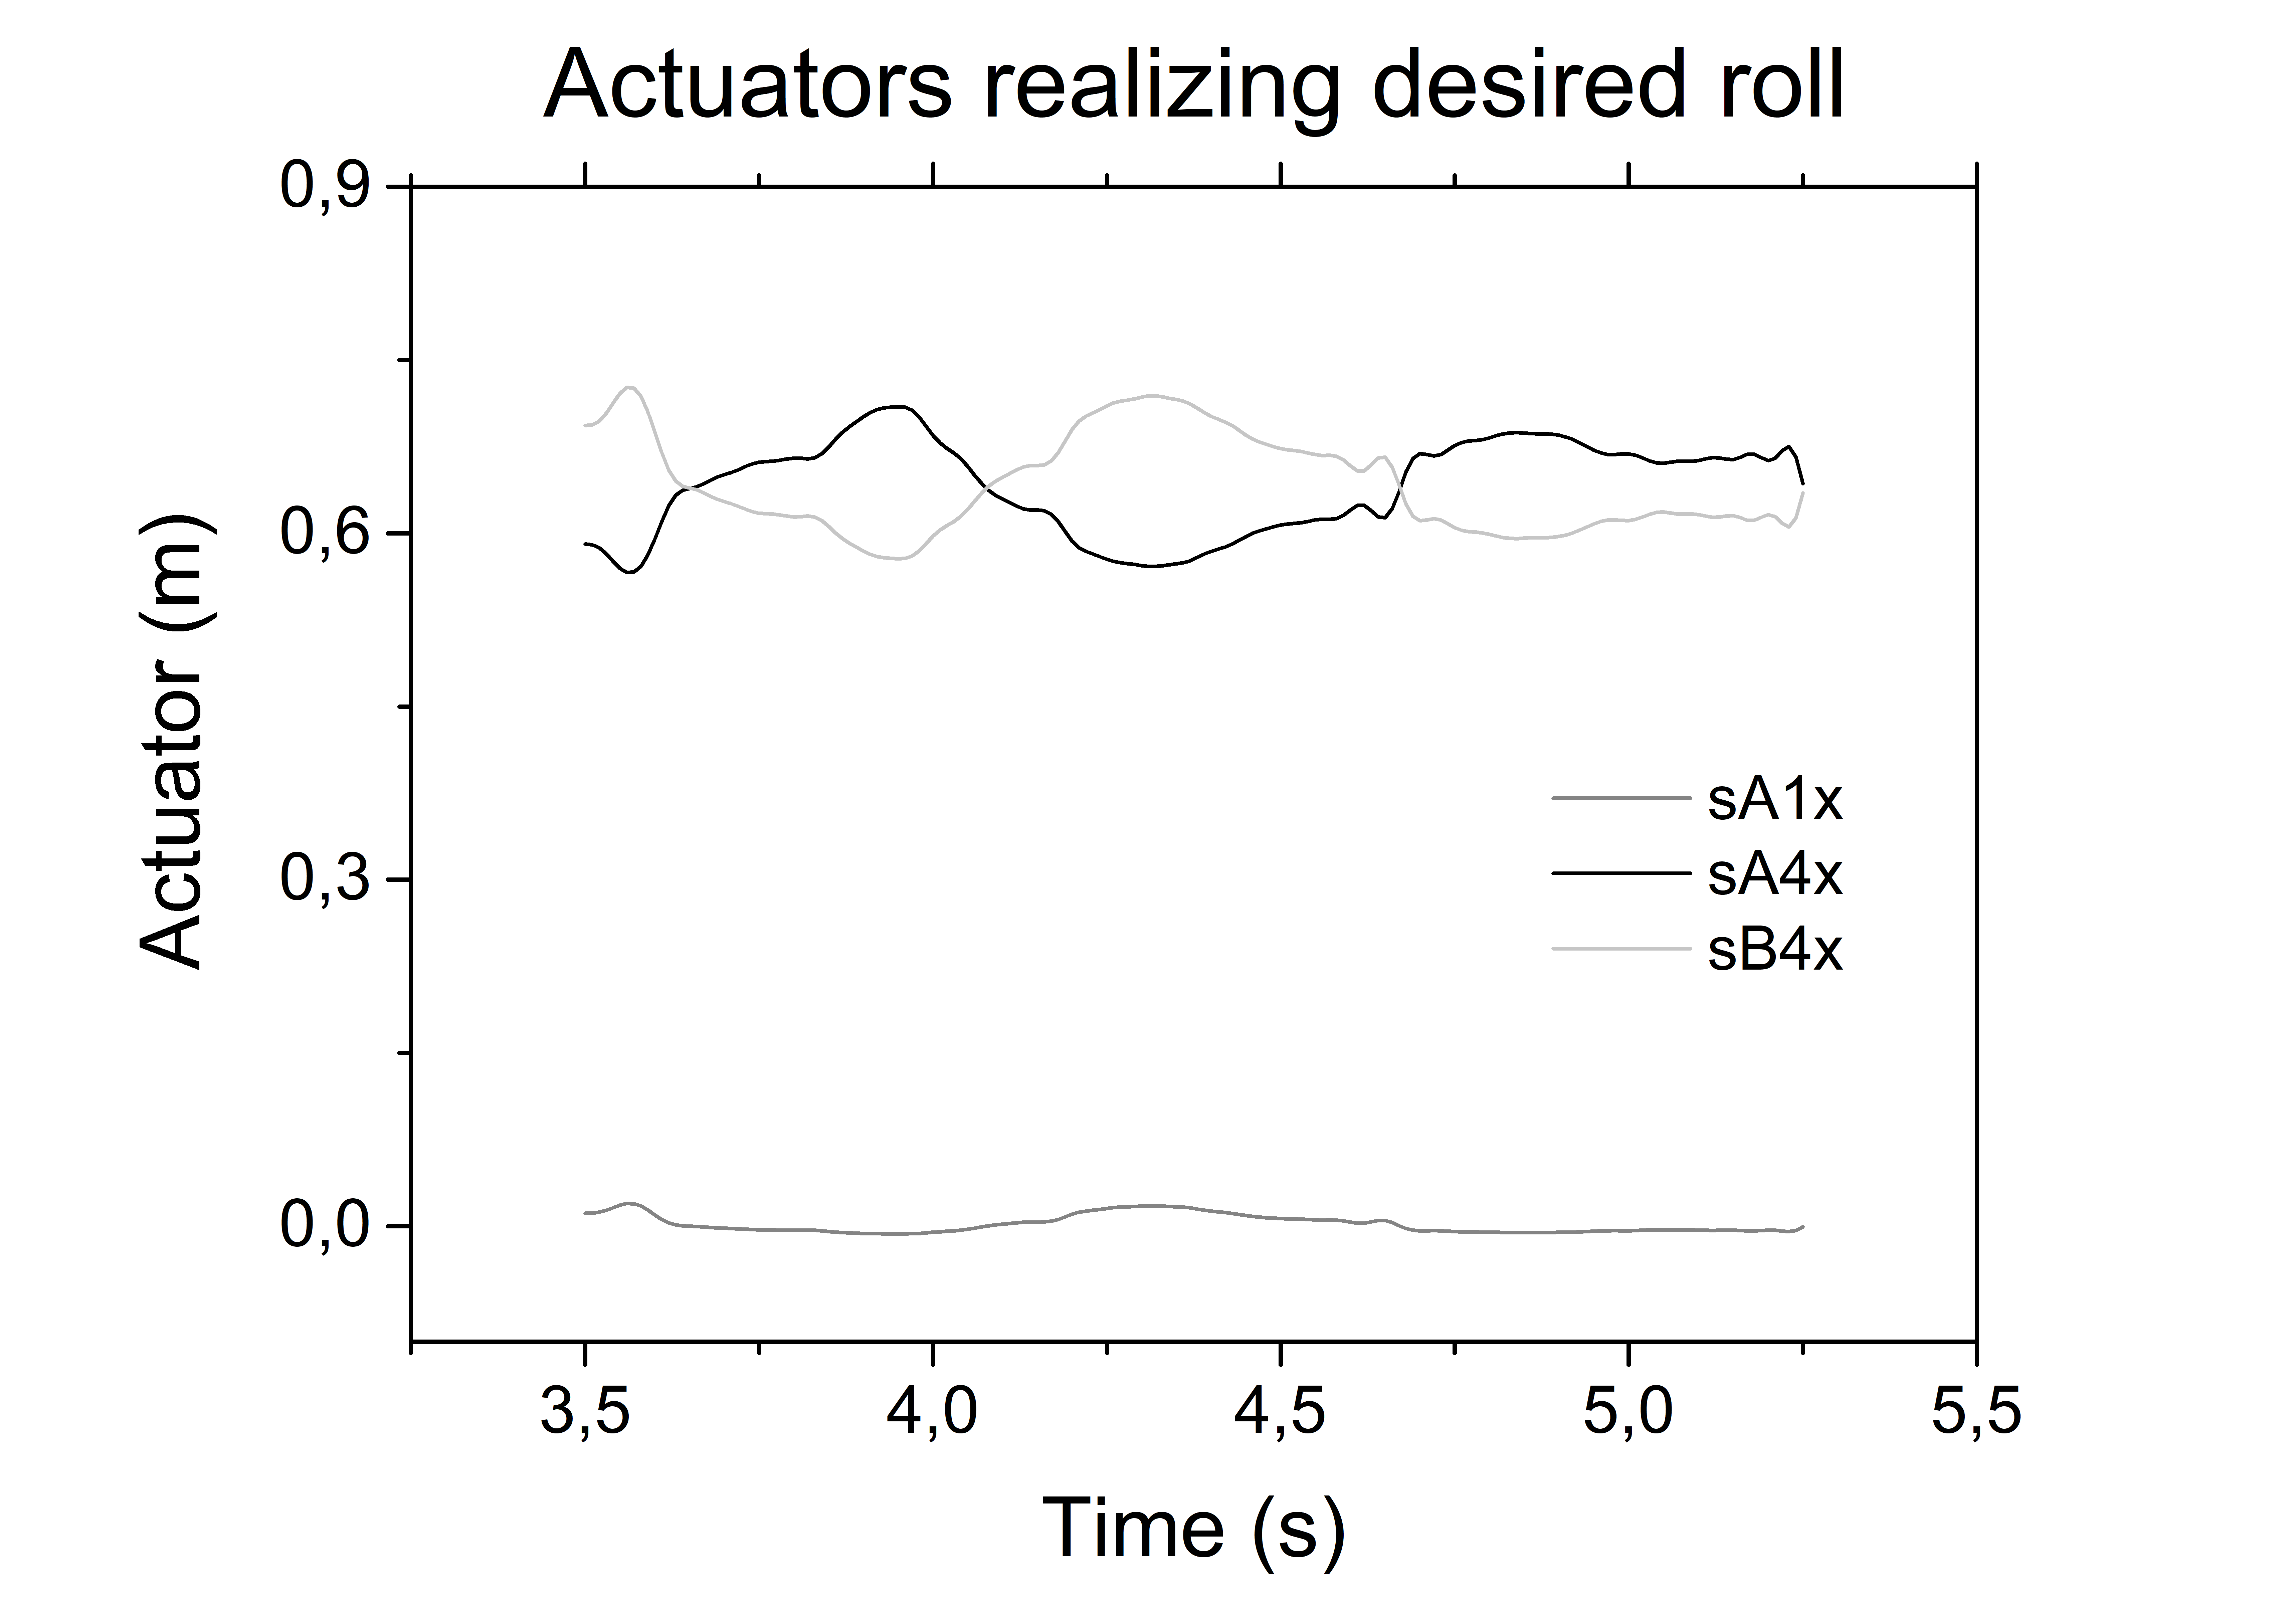
\includegraphics[width=7.5cm]{Images/Actuators_InvKine}
	\caption{Desired roll angle of the end effector (\( EE \)) and the consequent behaviour of the three actuators.}
  \label{fig:experimental}
\end{figure}


\section{Velocity analysis}
Regarding the velocity analysis the following approach has been followed.
At first, after having obtained from the position analysis the following three objects:
  \begin{itemize}
    \item \( \Phi_{tot}\): complete set of constraint equations;
    \item \( qI_{tot}\): set of independent variables;
    \item \( qD_{tot}\): set of dependent variables;
  \end{itemize}
three dependent variables (\( EE_{x}(t) \), \( EE_{y}(t) \) and \(EE_{angle}(t)\)) were added to the set of dependent variables and clearly to the set of constraint equations. The aim was to obtain directly the velocity ratios related to these variables, that are the \( x \) position, the \( y \) position and the roll angle of the center of mass of the platform that was tought as the position of an eventual driving position.
If that had not been done, velocity ratios would have been related  to other internal variables, such as the angles of the bars and the positions of the rolleys.

The Jacobians w.r.t. the dependent and independent coordinates have been computed and thus the matrix of velocity ratios \([ \tau ]\) was calculated exploiting the Jacobians, as it is shown below \cite{Biral}:
  \begin{equation}
    \left[\frac{\partial \Phi }{\partial q_I}\right] \cdot \dot{q_I} + \left[\frac{\partial \Phi }{\partial q_D}\right] \cdot \dot{q_D'} = 0
  \end{equation}

  \begin{equation}
    \dot{q_D} = -\left[\frac{\partial \Phi }{\partial q_D}\right]^{-1} \cdot \left[\frac{\partial \Phi }{\partial q_I}\right] \cdot \dot{q_I}
  \end{equation}

  \begin{equation}
    \tau = - \left[\frac{\partial \Phi }{\partial q_D}\right]^{-1} \cdot \left[\frac{\partial \Phi }{\partial q_I}\right]
  \end{equation}
The velocity ratios are shown in Figure \ref{fig:v_r} only as function of actuator \(A4\), as an example. It's important to note that the points where the ratios goes to infinity, indicative of non-assembling mechanism, are far away from the extremes found with the procedure shown in Section \ref{s:Extreme-positions}.

Later on, it was calculated analitically the velocities of the dependent coordinates solving the derivative w.r.t. time of the equations of the complete set of constraints considering as unkonwns the derivative w.r.t. time of the complete set of dependent coordinates. Then, in the obtained solution, it was substituted the solution of the kinematics found in Section \ref{s:Direct-position}.

In Figure \ref{fig:vel} are shown the pure velocities of the \( x \), \( y \) position of the end effector and its roll angle w.r.t. the position of one of the three DoF. In this case the velocity of the active actuator was fixed to one while the position of the other two actuators was mantained in the initial position.


\newgeometry{left=1.7cm,right=1.7cm,top=2.7cm,bottom=2.7cm}
\begin{figure*}
\centering
\begin{minipage}{0.49\textwidth}
	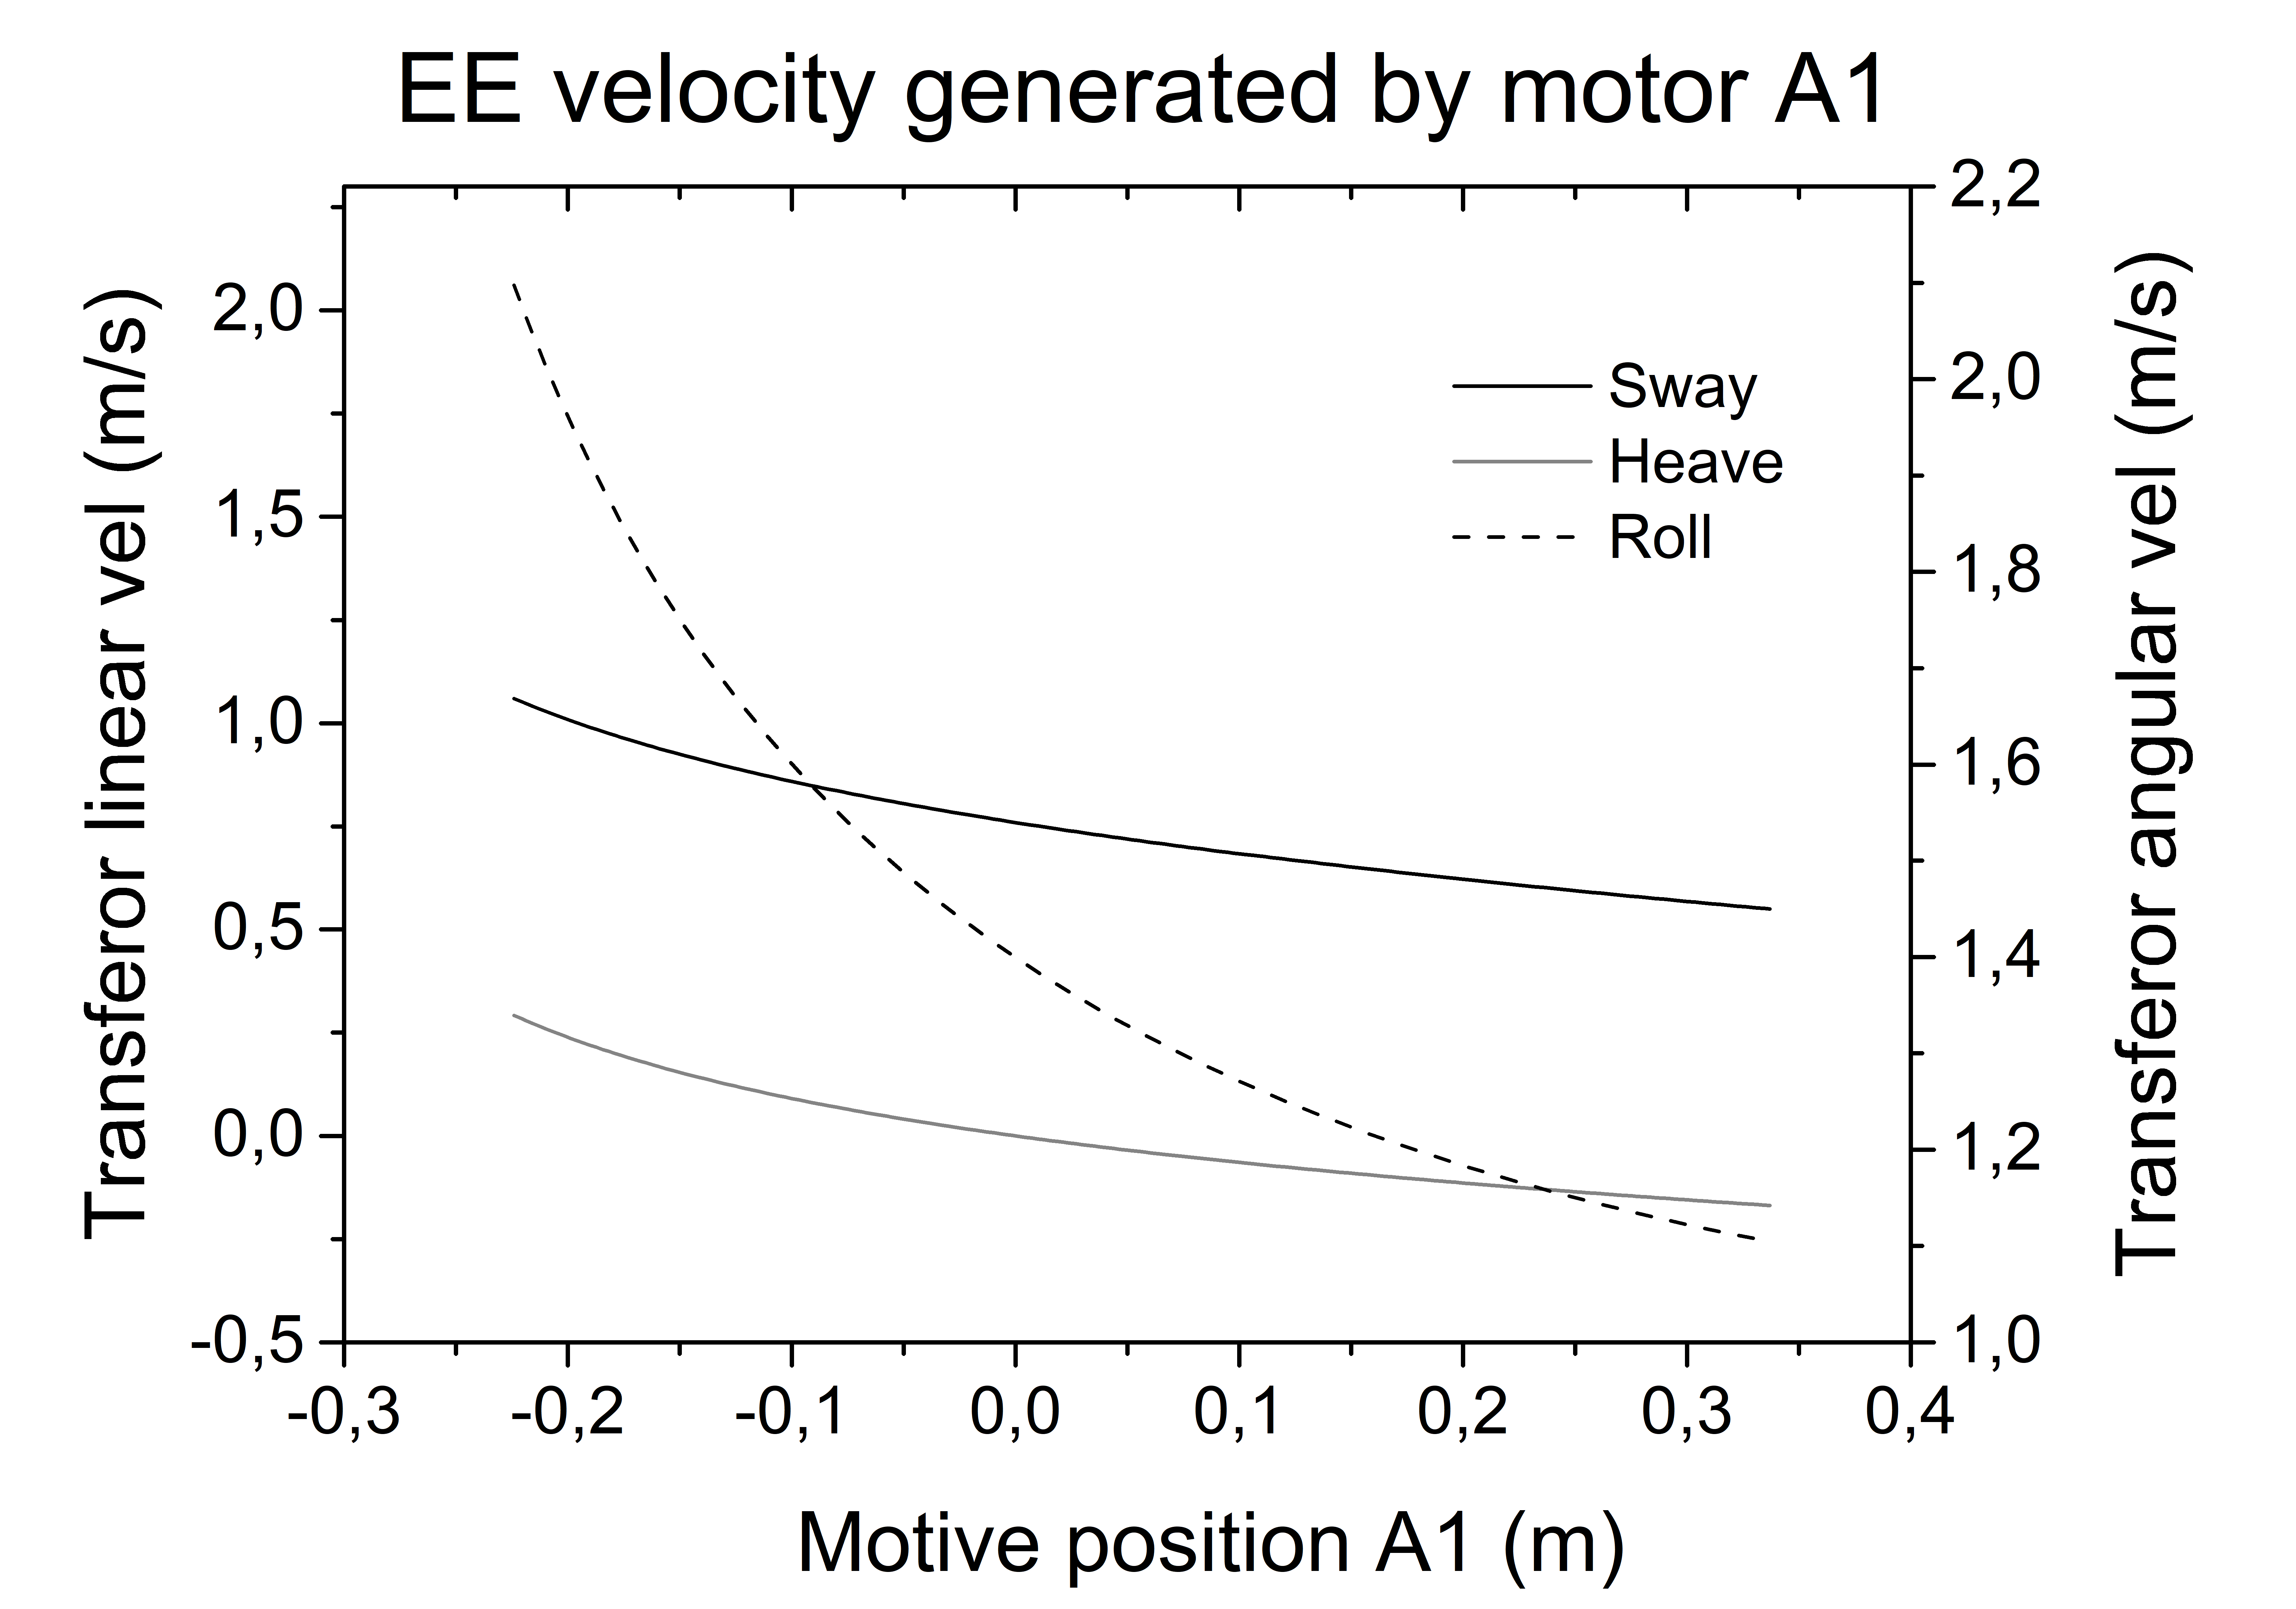
\includegraphics[width=7.5cm]{Images/EE_vel_A1}
\end{minipage}
\begin{minipage}{0.49\textwidth}
	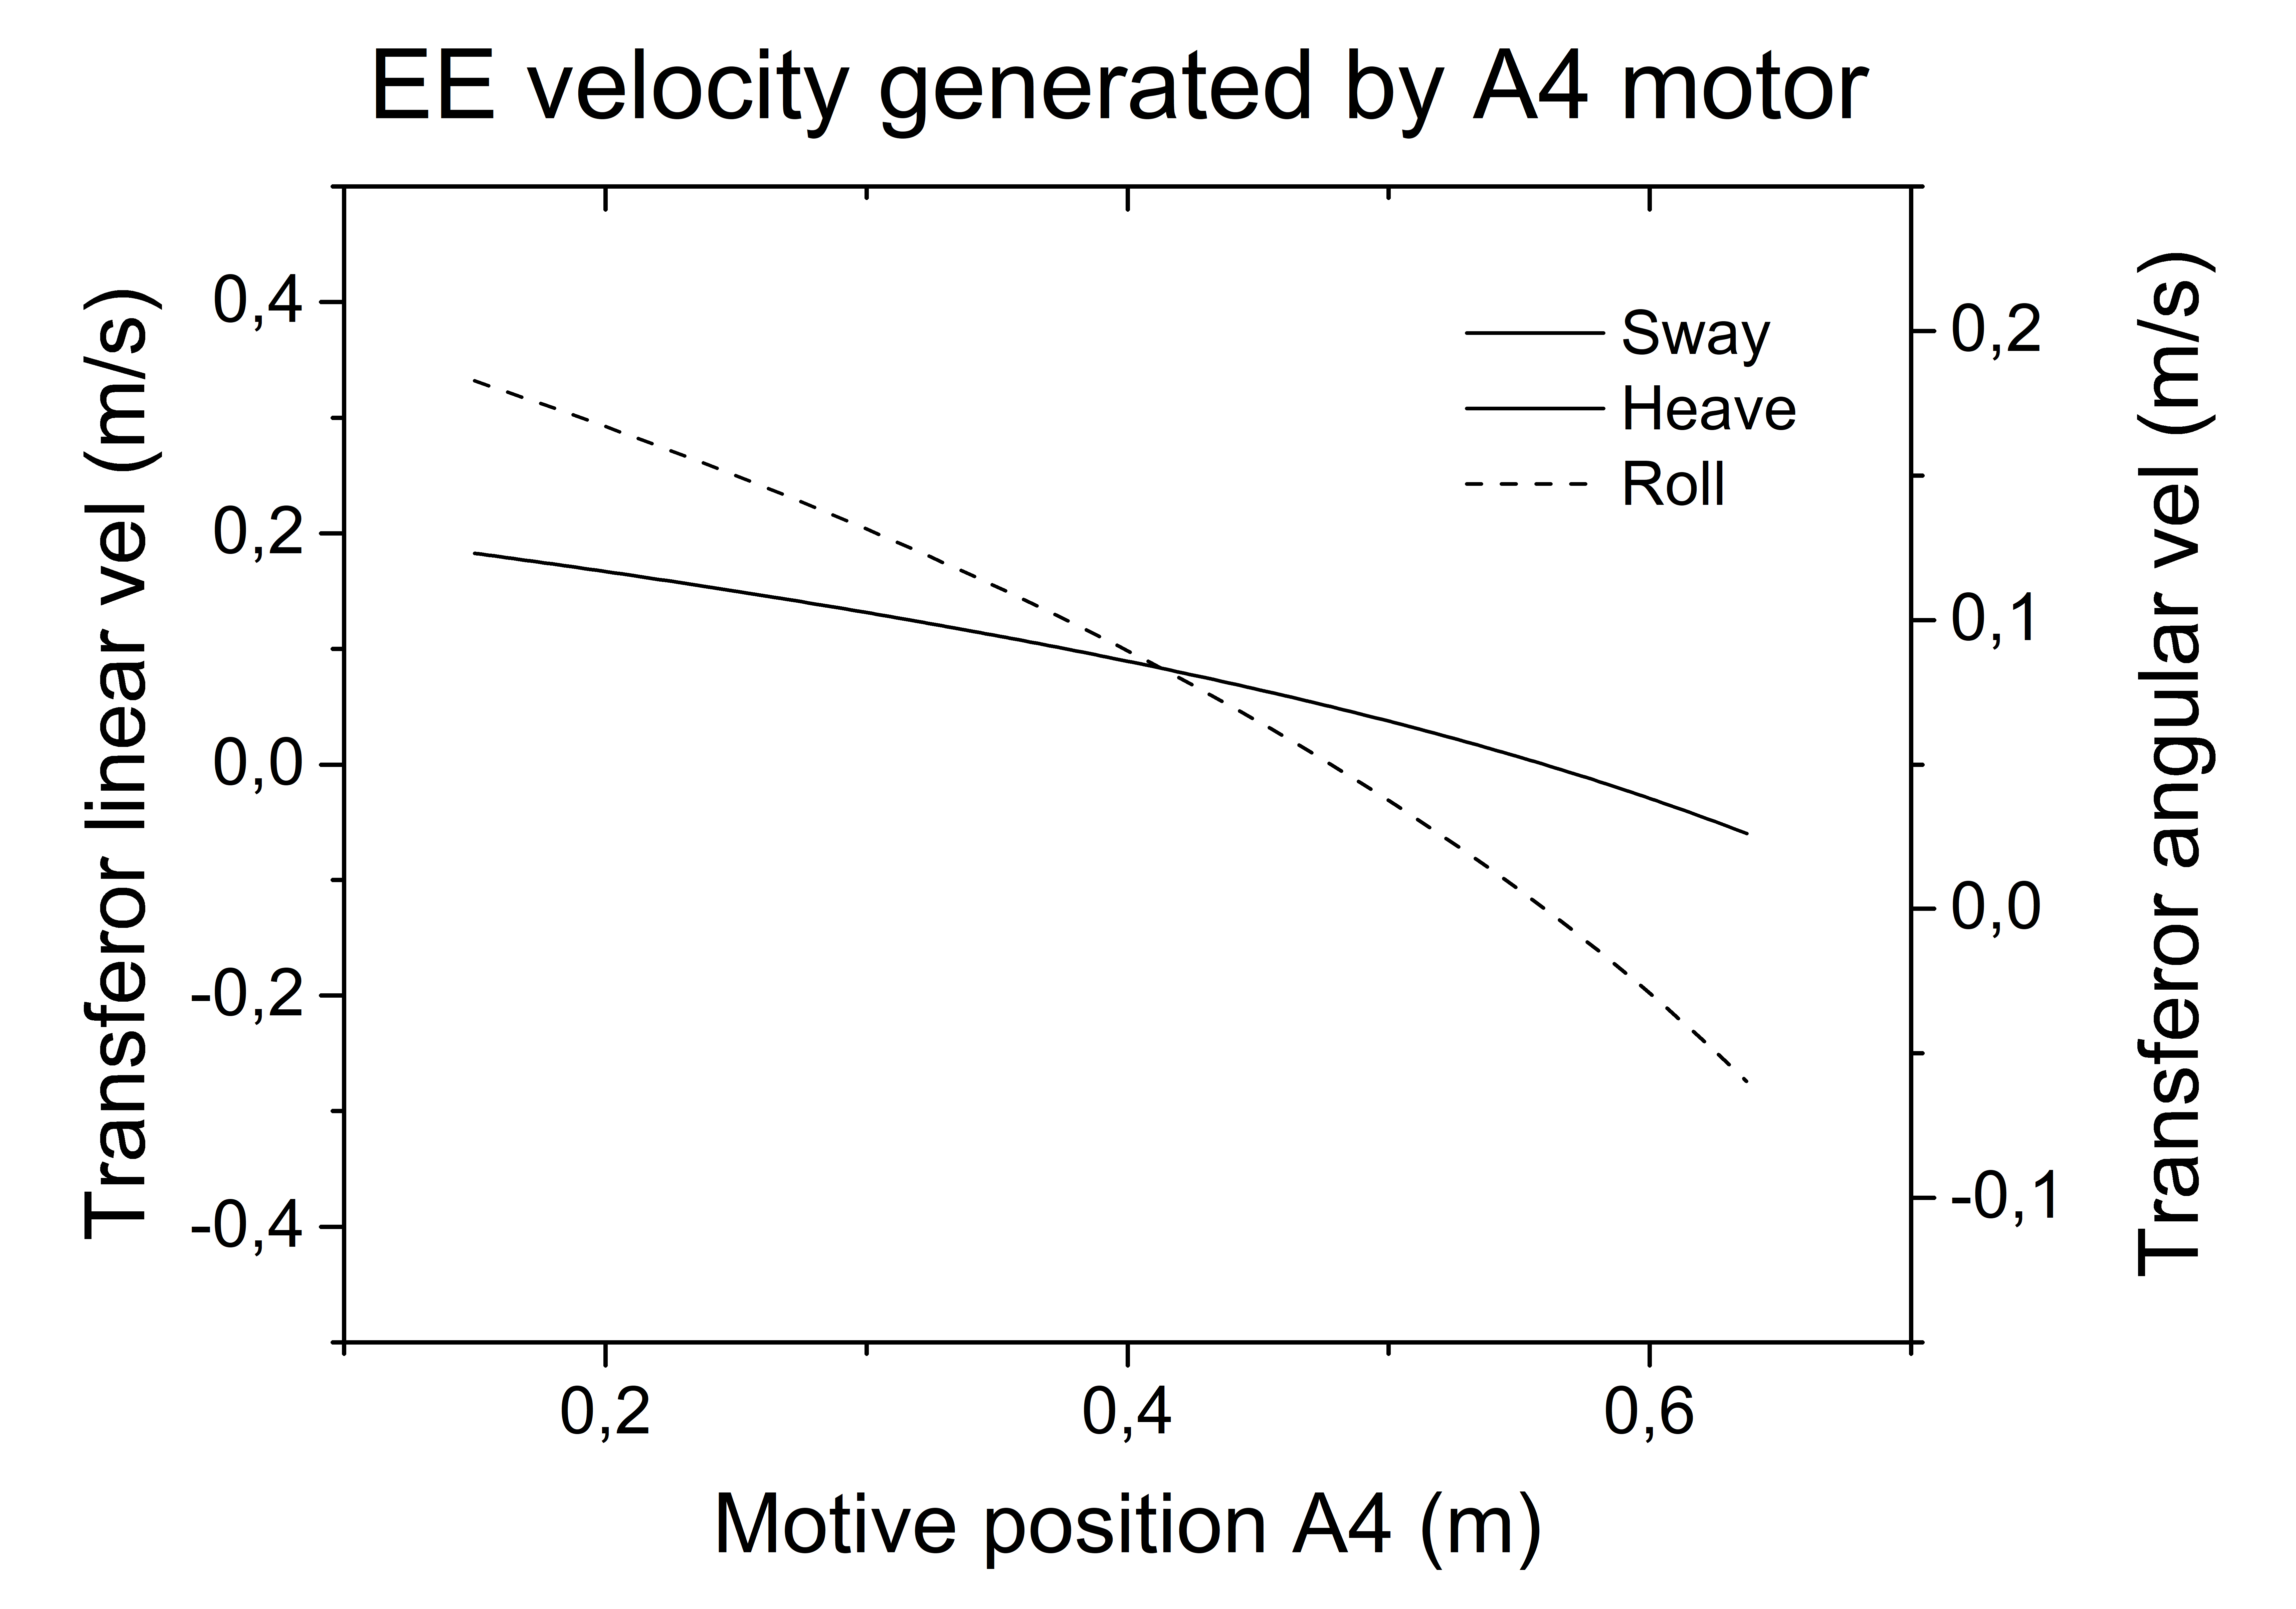
\includegraphics[width=7.5cm]{Images/EE_vel_A4}
\end{minipage}
\begin{minipage}{0.49\textwidth}
	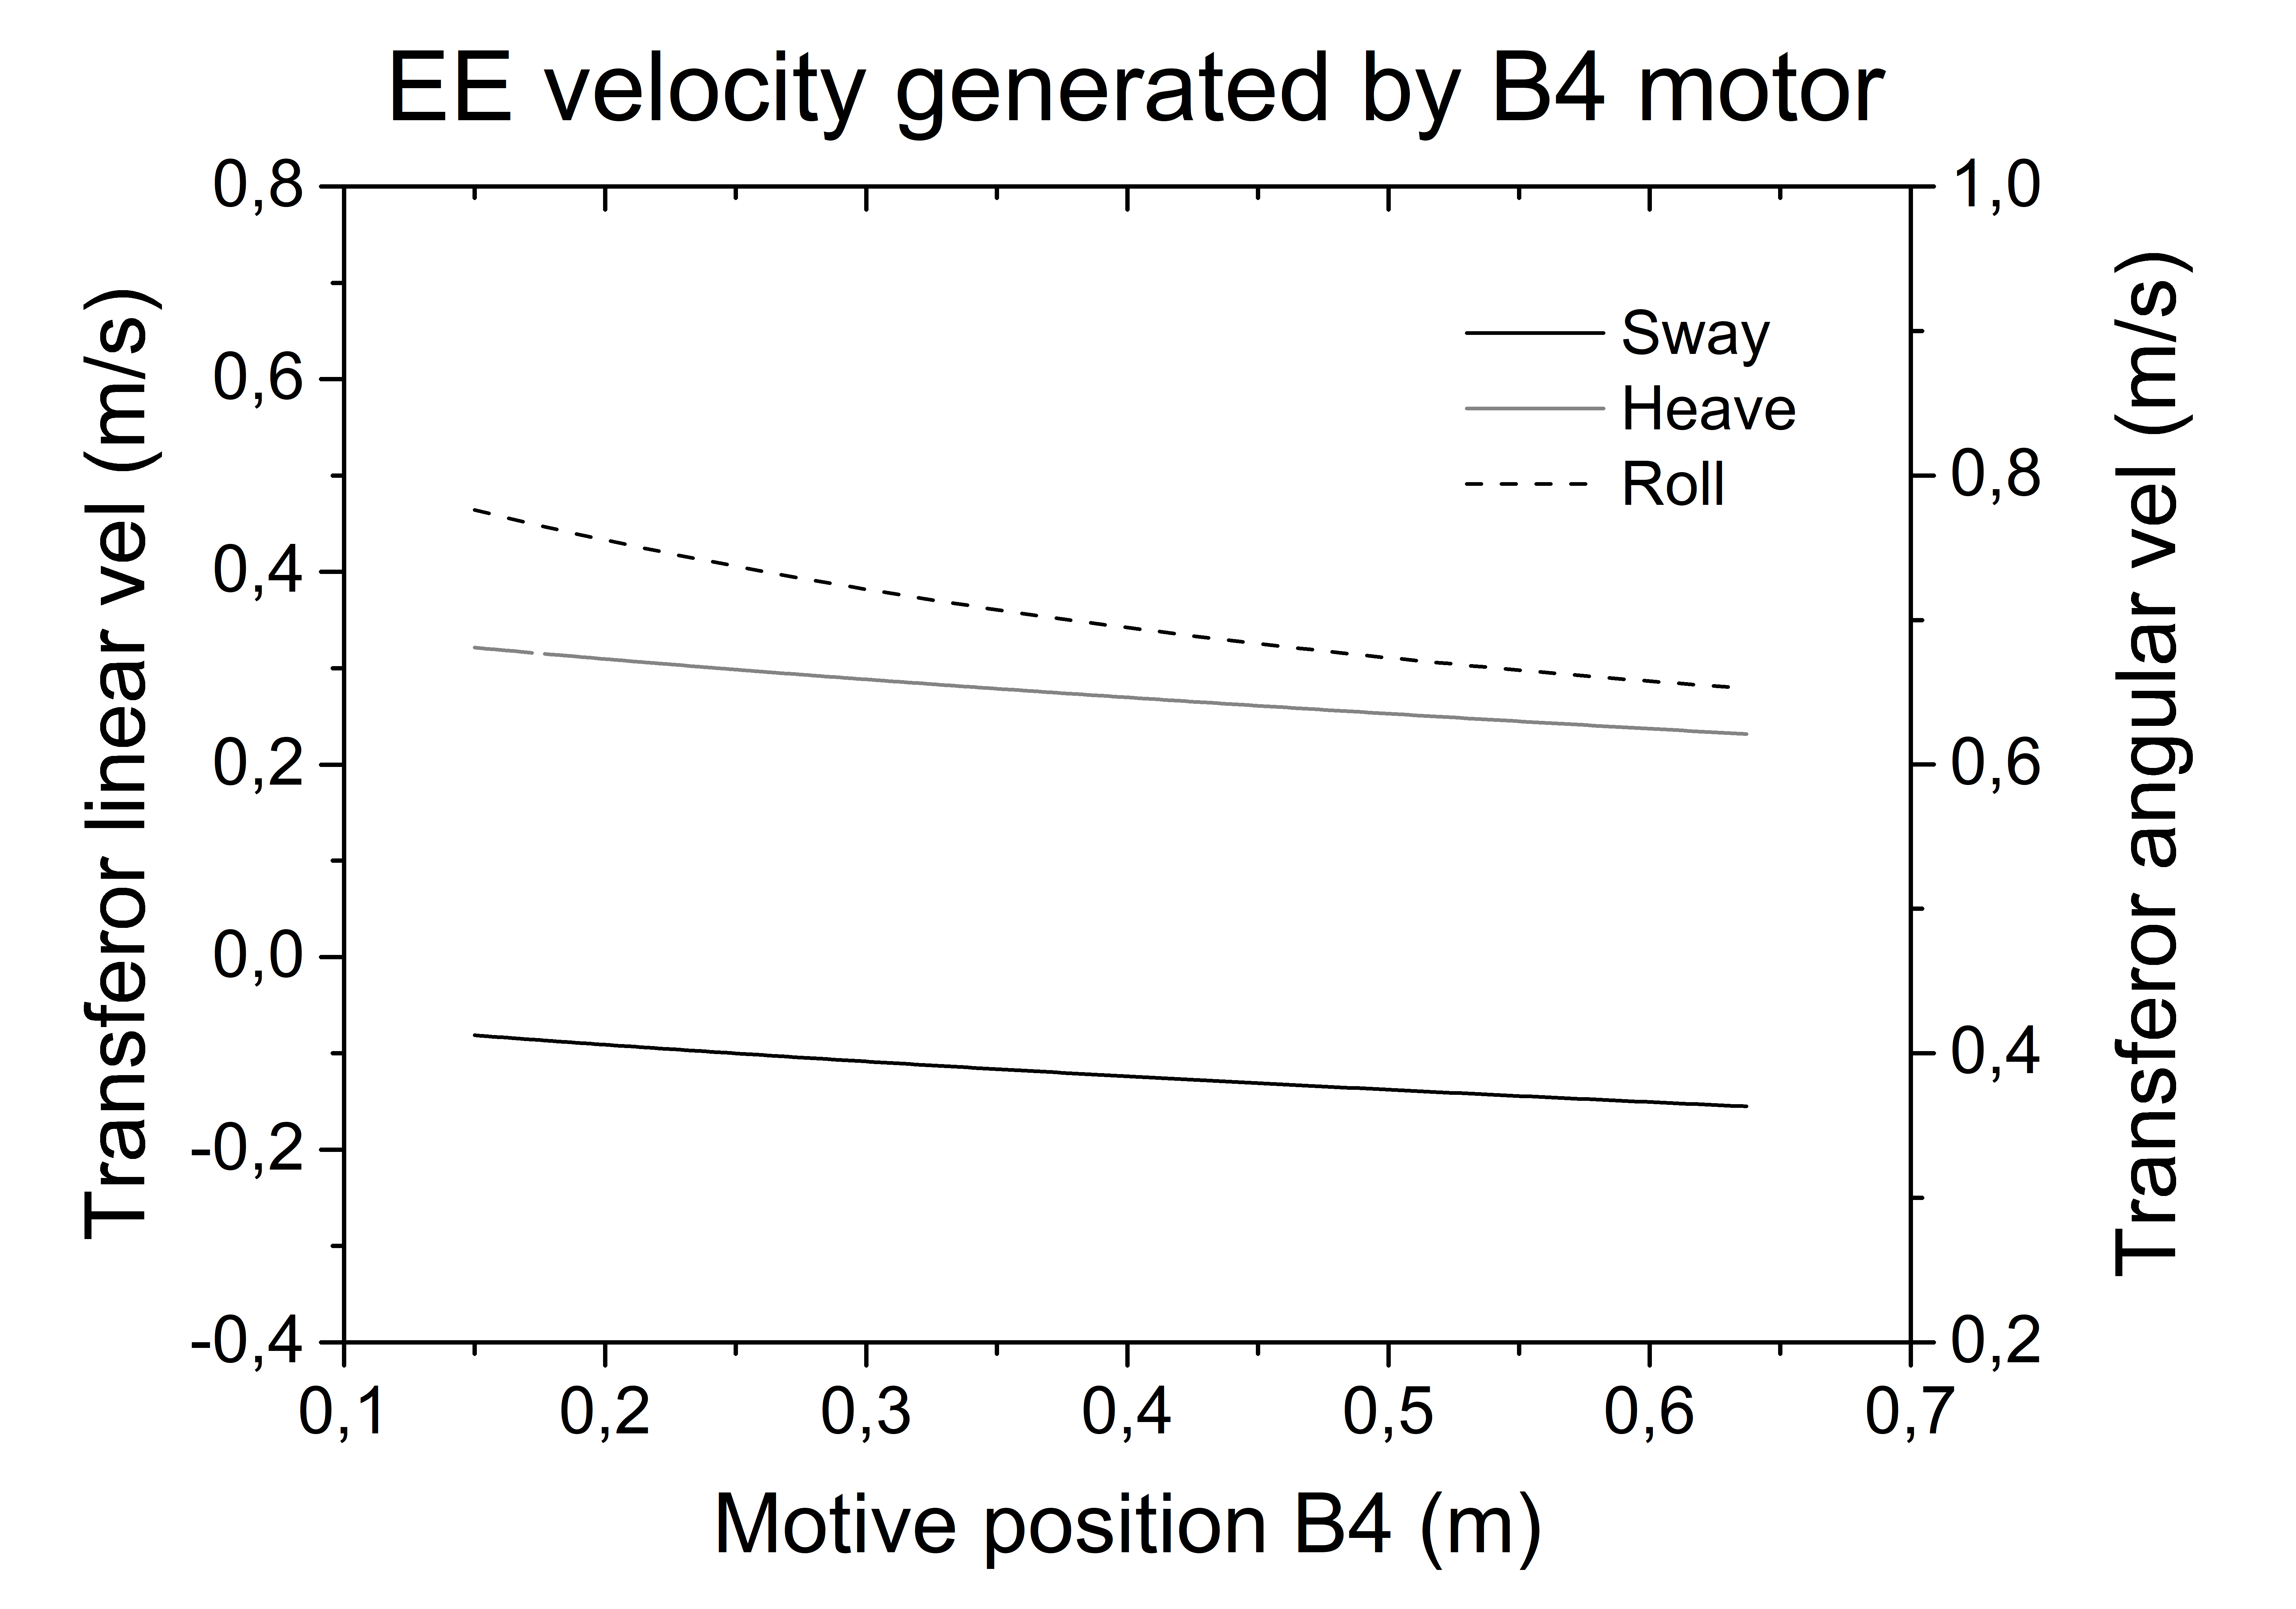
\includegraphics[width=7.5cm]{Images/EE_vel_B4}
\end{minipage}
    \caption{Velocity of the end effector (\( EE \)) as a function of the actuator positions.}
     \label{fig:vel}
\end{figure*}

\begin{figure*}
\centering
\begin{minipage}{0.49\textwidth}
	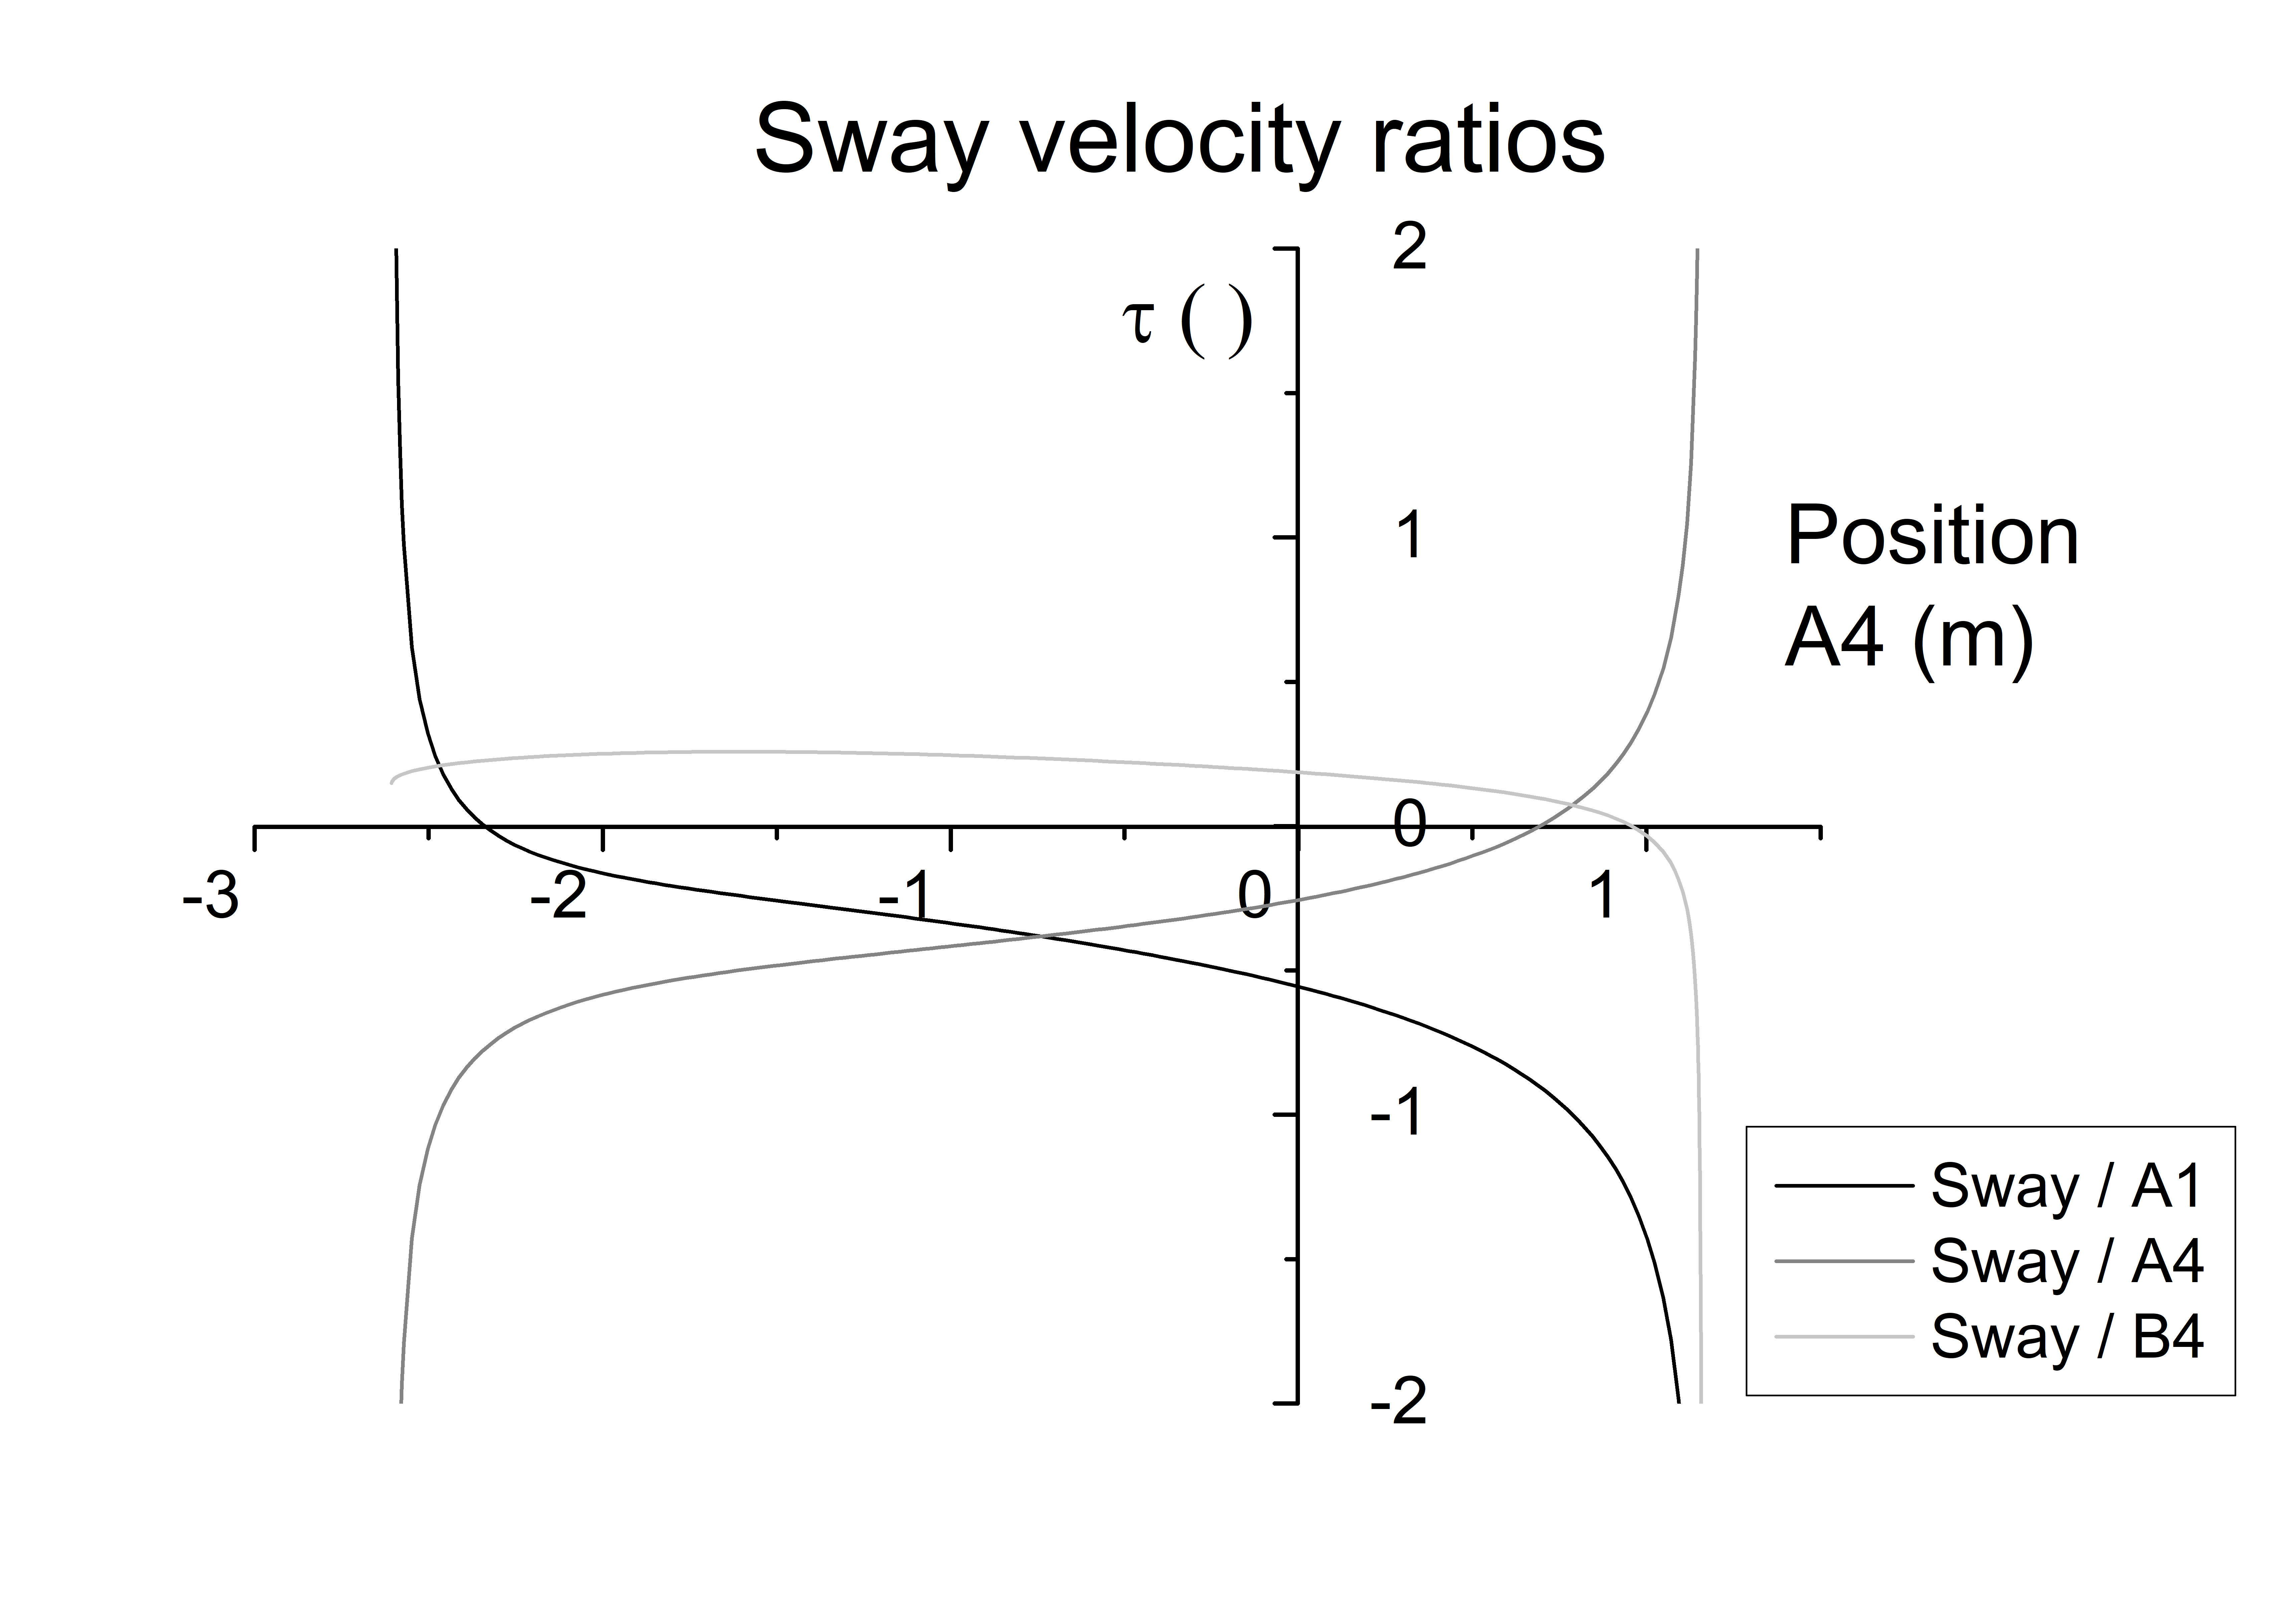
\includegraphics[width=7.5cm]{Images/Ratio_x}
\end{minipage}
\begin{minipage}{0.49\textwidth}
	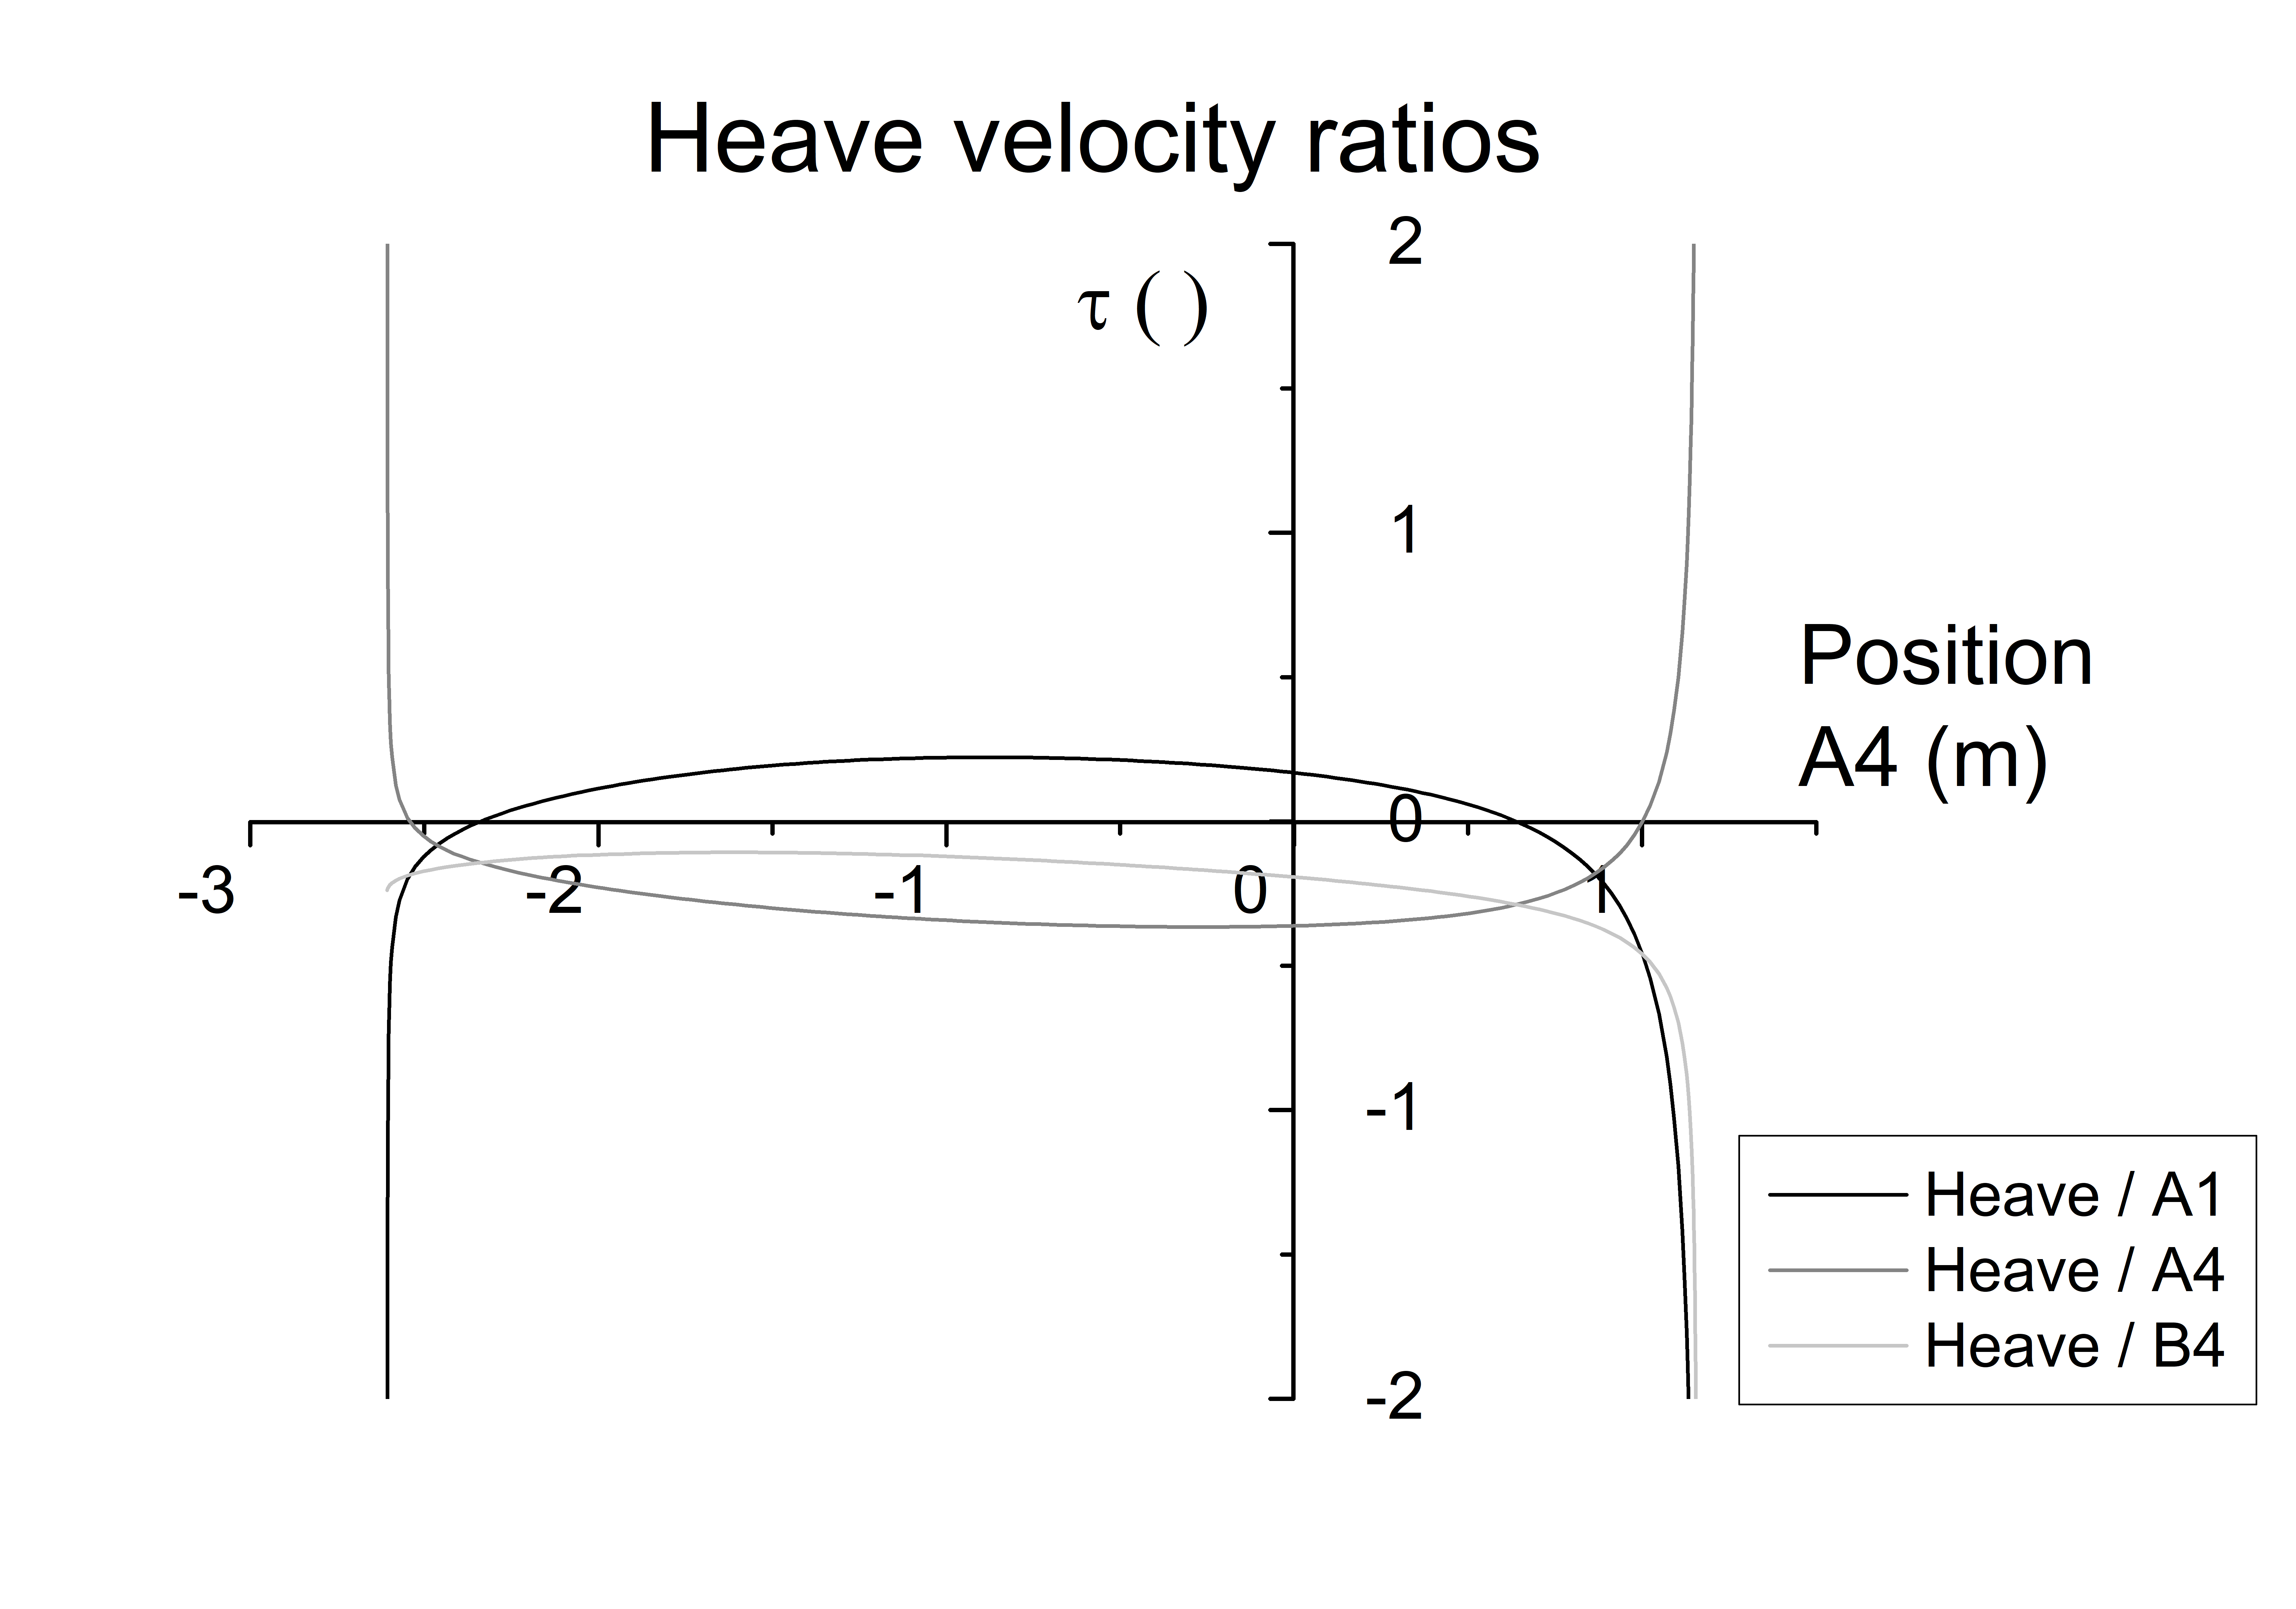
\includegraphics[width=7.5cm]{Images/Ratio_y}
\end{minipage}
\begin{minipage}{0.49\textwidth}
	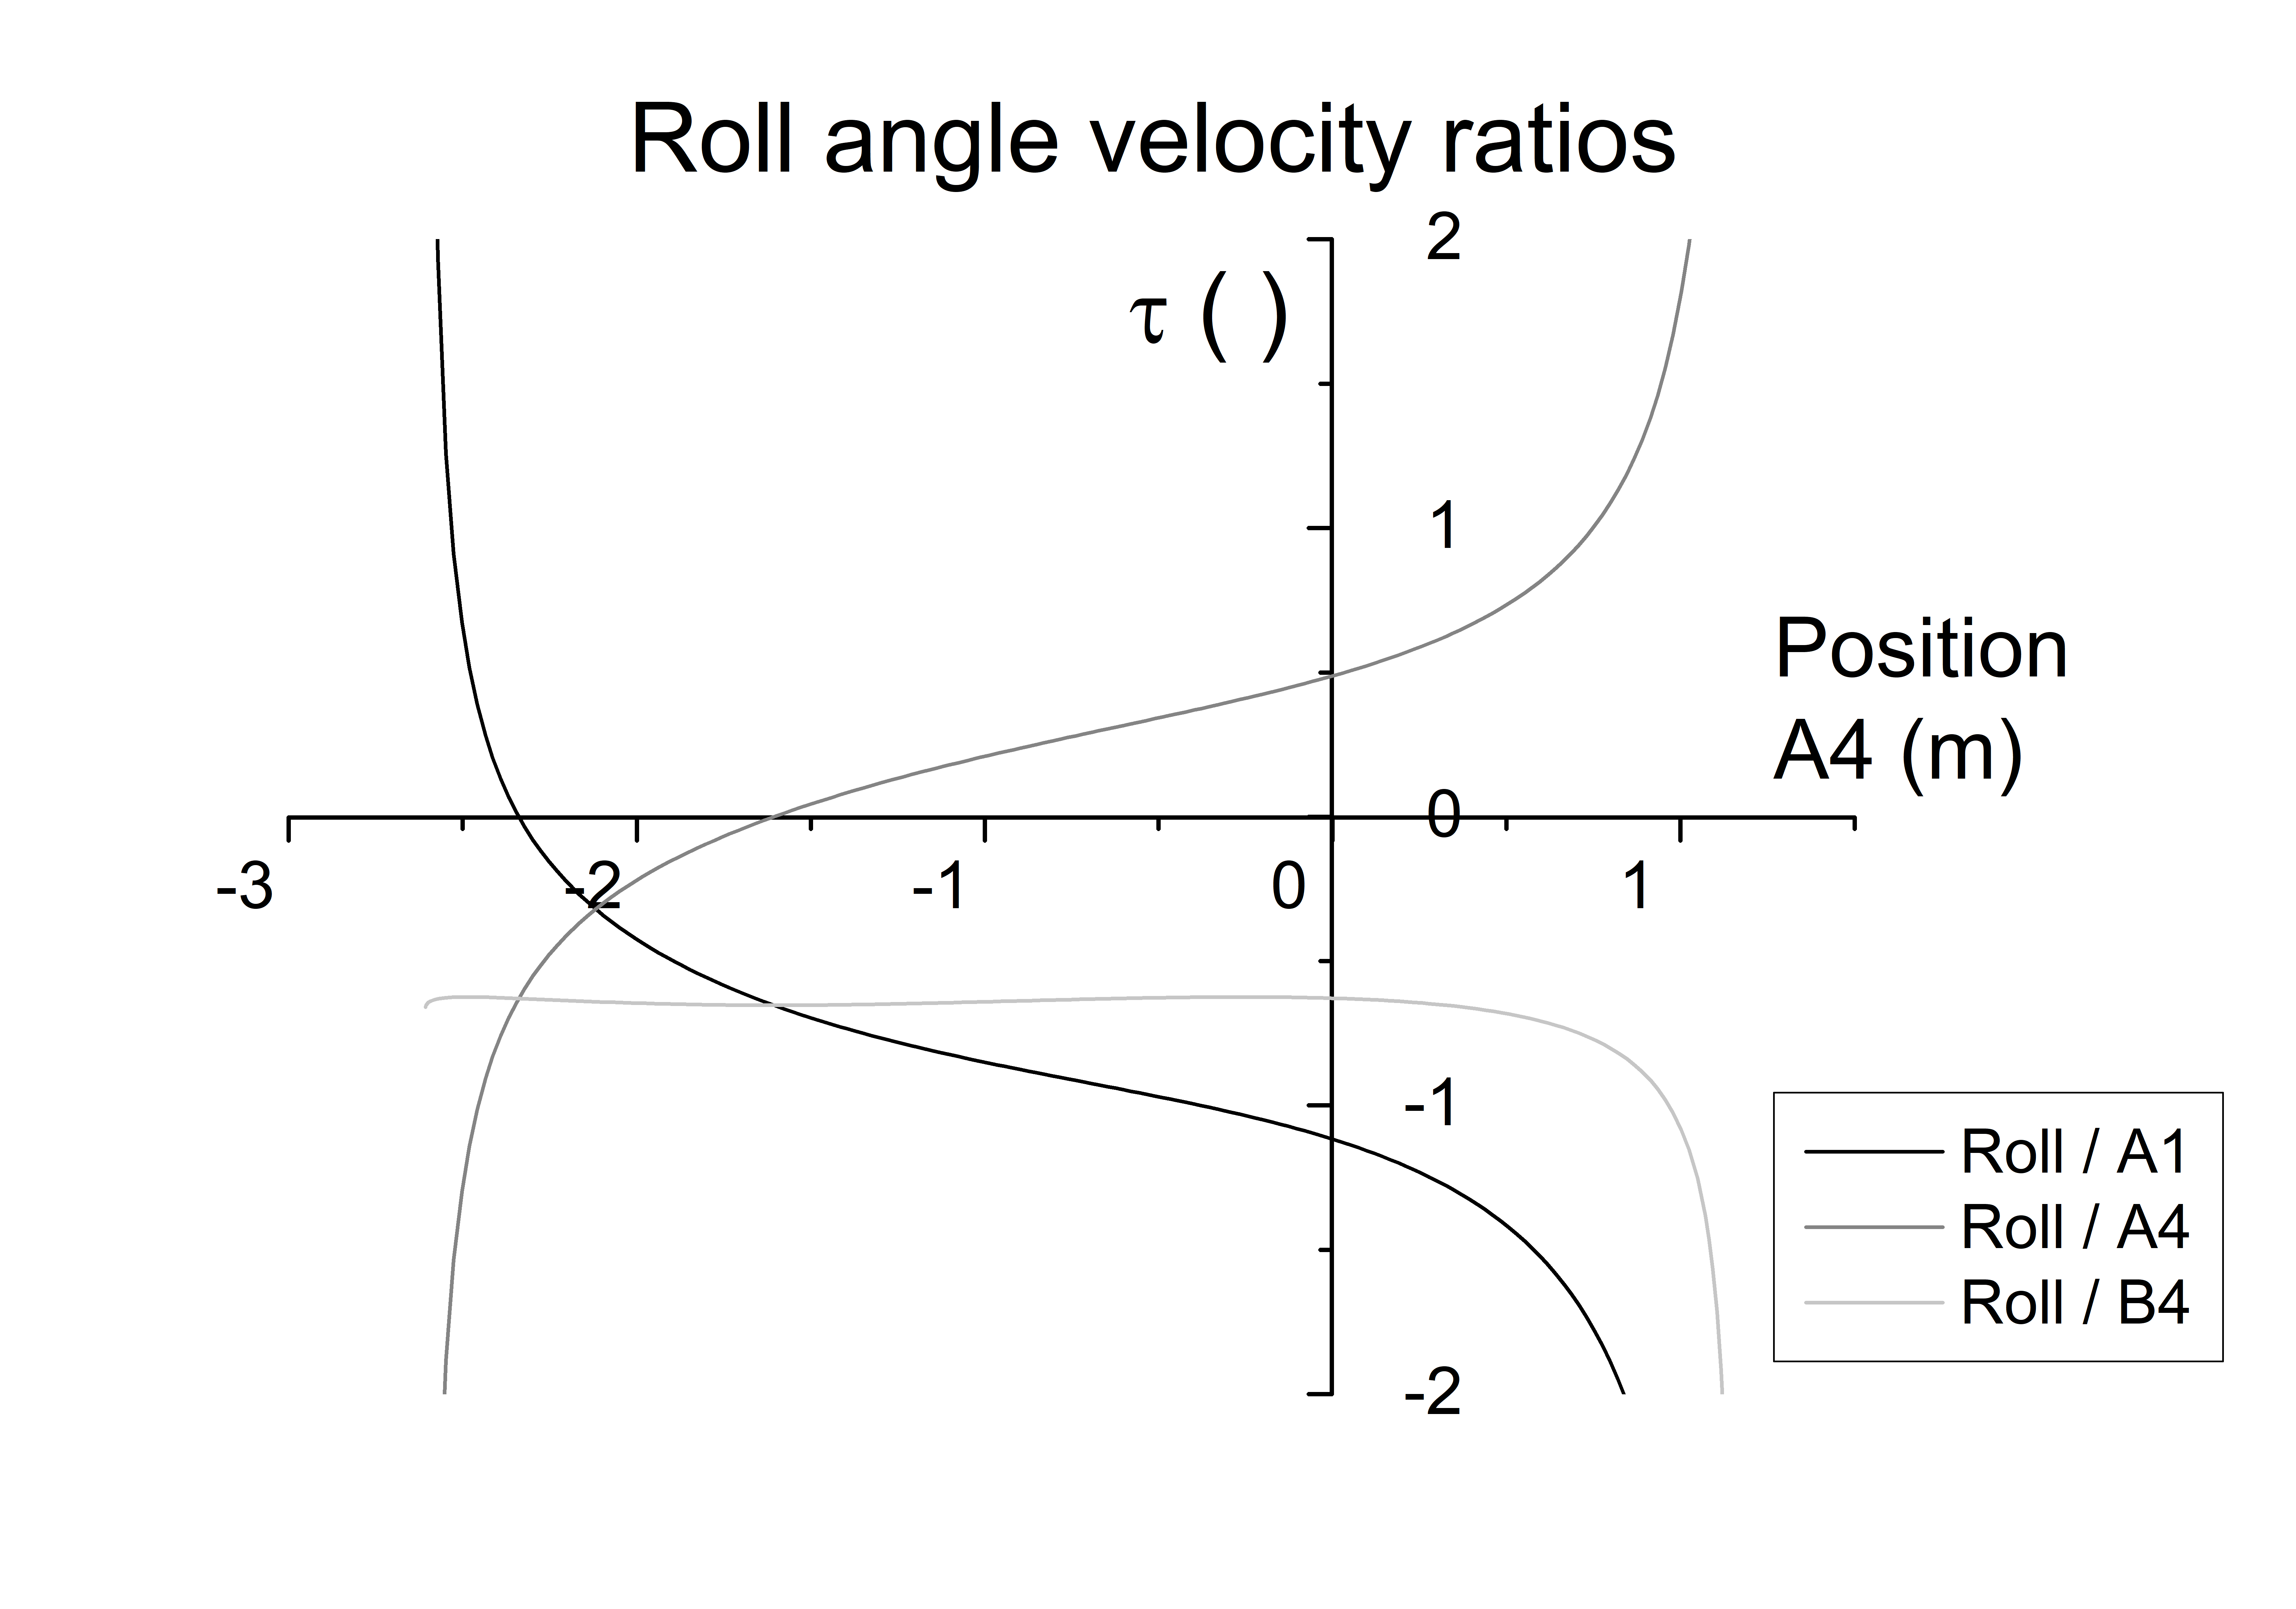
\includegraphics[width=7.5cm]{Images/Ratio_angle}
\end{minipage}
    \caption{Velocity ratios of the end effector (\( EE \)).}
 \label{fig:v_r}
\end{figure*}
\clearpage
\restoregeometry




\section{Acceleration analysis}
The development of this part has been quite similar to the one made in the previous section.

Having the analitical solution of the kinematics, in order to obtain the expression of the acceleration of the dependent coordinates it was solved the double derivative w.r.t. time of the complete set of constraints considering as unkonwns the double derivative w.r.t. time of the complete set of dependent coordinates.

After that, the chosen solution of the kinematics was substituted into the expression of the dependent acceleration in order to obtain them as dependent only to the independent variables.

In Figure \ref{fig:acc} the acceleration of the \( x \), \( y \) coordinates and of the roll angle of the end effector is plotted w.r.t the position of each one of the three DoF (mantaining the other two fixed at each time). Furthermore, the velocity and the acceleration of the moving actuator, were fixed to the unitary value.

  \begin{multline}
    \left[\frac{\partial \Phi }{\partial q_D}\right] \cdot \ddot{q_D} = - \frac{d}{dt} \left(\left[\frac{\partial \Phi }{\partial q_I}\right] \cdot \dot{q_I} \right) -\\
    - \frac{d}{dt} \left(\left[\frac{\partial \Phi }{\partial q_D}\right] \cdot \dot{q_D} \right)
  \end{multline}

After some derivation the final equation, that shows the components of the dependent accelerations, can be written as:
  \begin{multline}
    \ddot{q_D} = -\left[\frac{\partial \Phi }{\partial q_D}\right]^{-1} \cdot \\ \left(\left[\frac{\partial \Phi }{\partial q_I}\right] \cdot \ddot{q_I} + \left[D(q_I)\right] \cdot \dot{q_I}^{2} \right)
  \end{multline}
where the matrix \([D(q_I)]\), that is a function of the independent coordinates, can be written as:
  \begin{multline}
    \bigg(\Big[\nabla_{a_{D}}\Big] \otimes \dot{q_{D}}
    + \Big[\nabla_{a_{I}}\Big] \otimes \dot{q_{I}}\Big] \bigg) \cdot
    \dot{q_{D}} -\\
    - \bigg(\Big[\nabla_{q_{D}}\Big] \otimes \dot{q_{D}}
    + \Big[\nabla_{b_{I}}\Big] \otimes
    \dot{q_{I}} \Big] \cdot
    \dot{q_{I}}
    \bigg)
  \end{multline}

\begin{figure}[h!]
	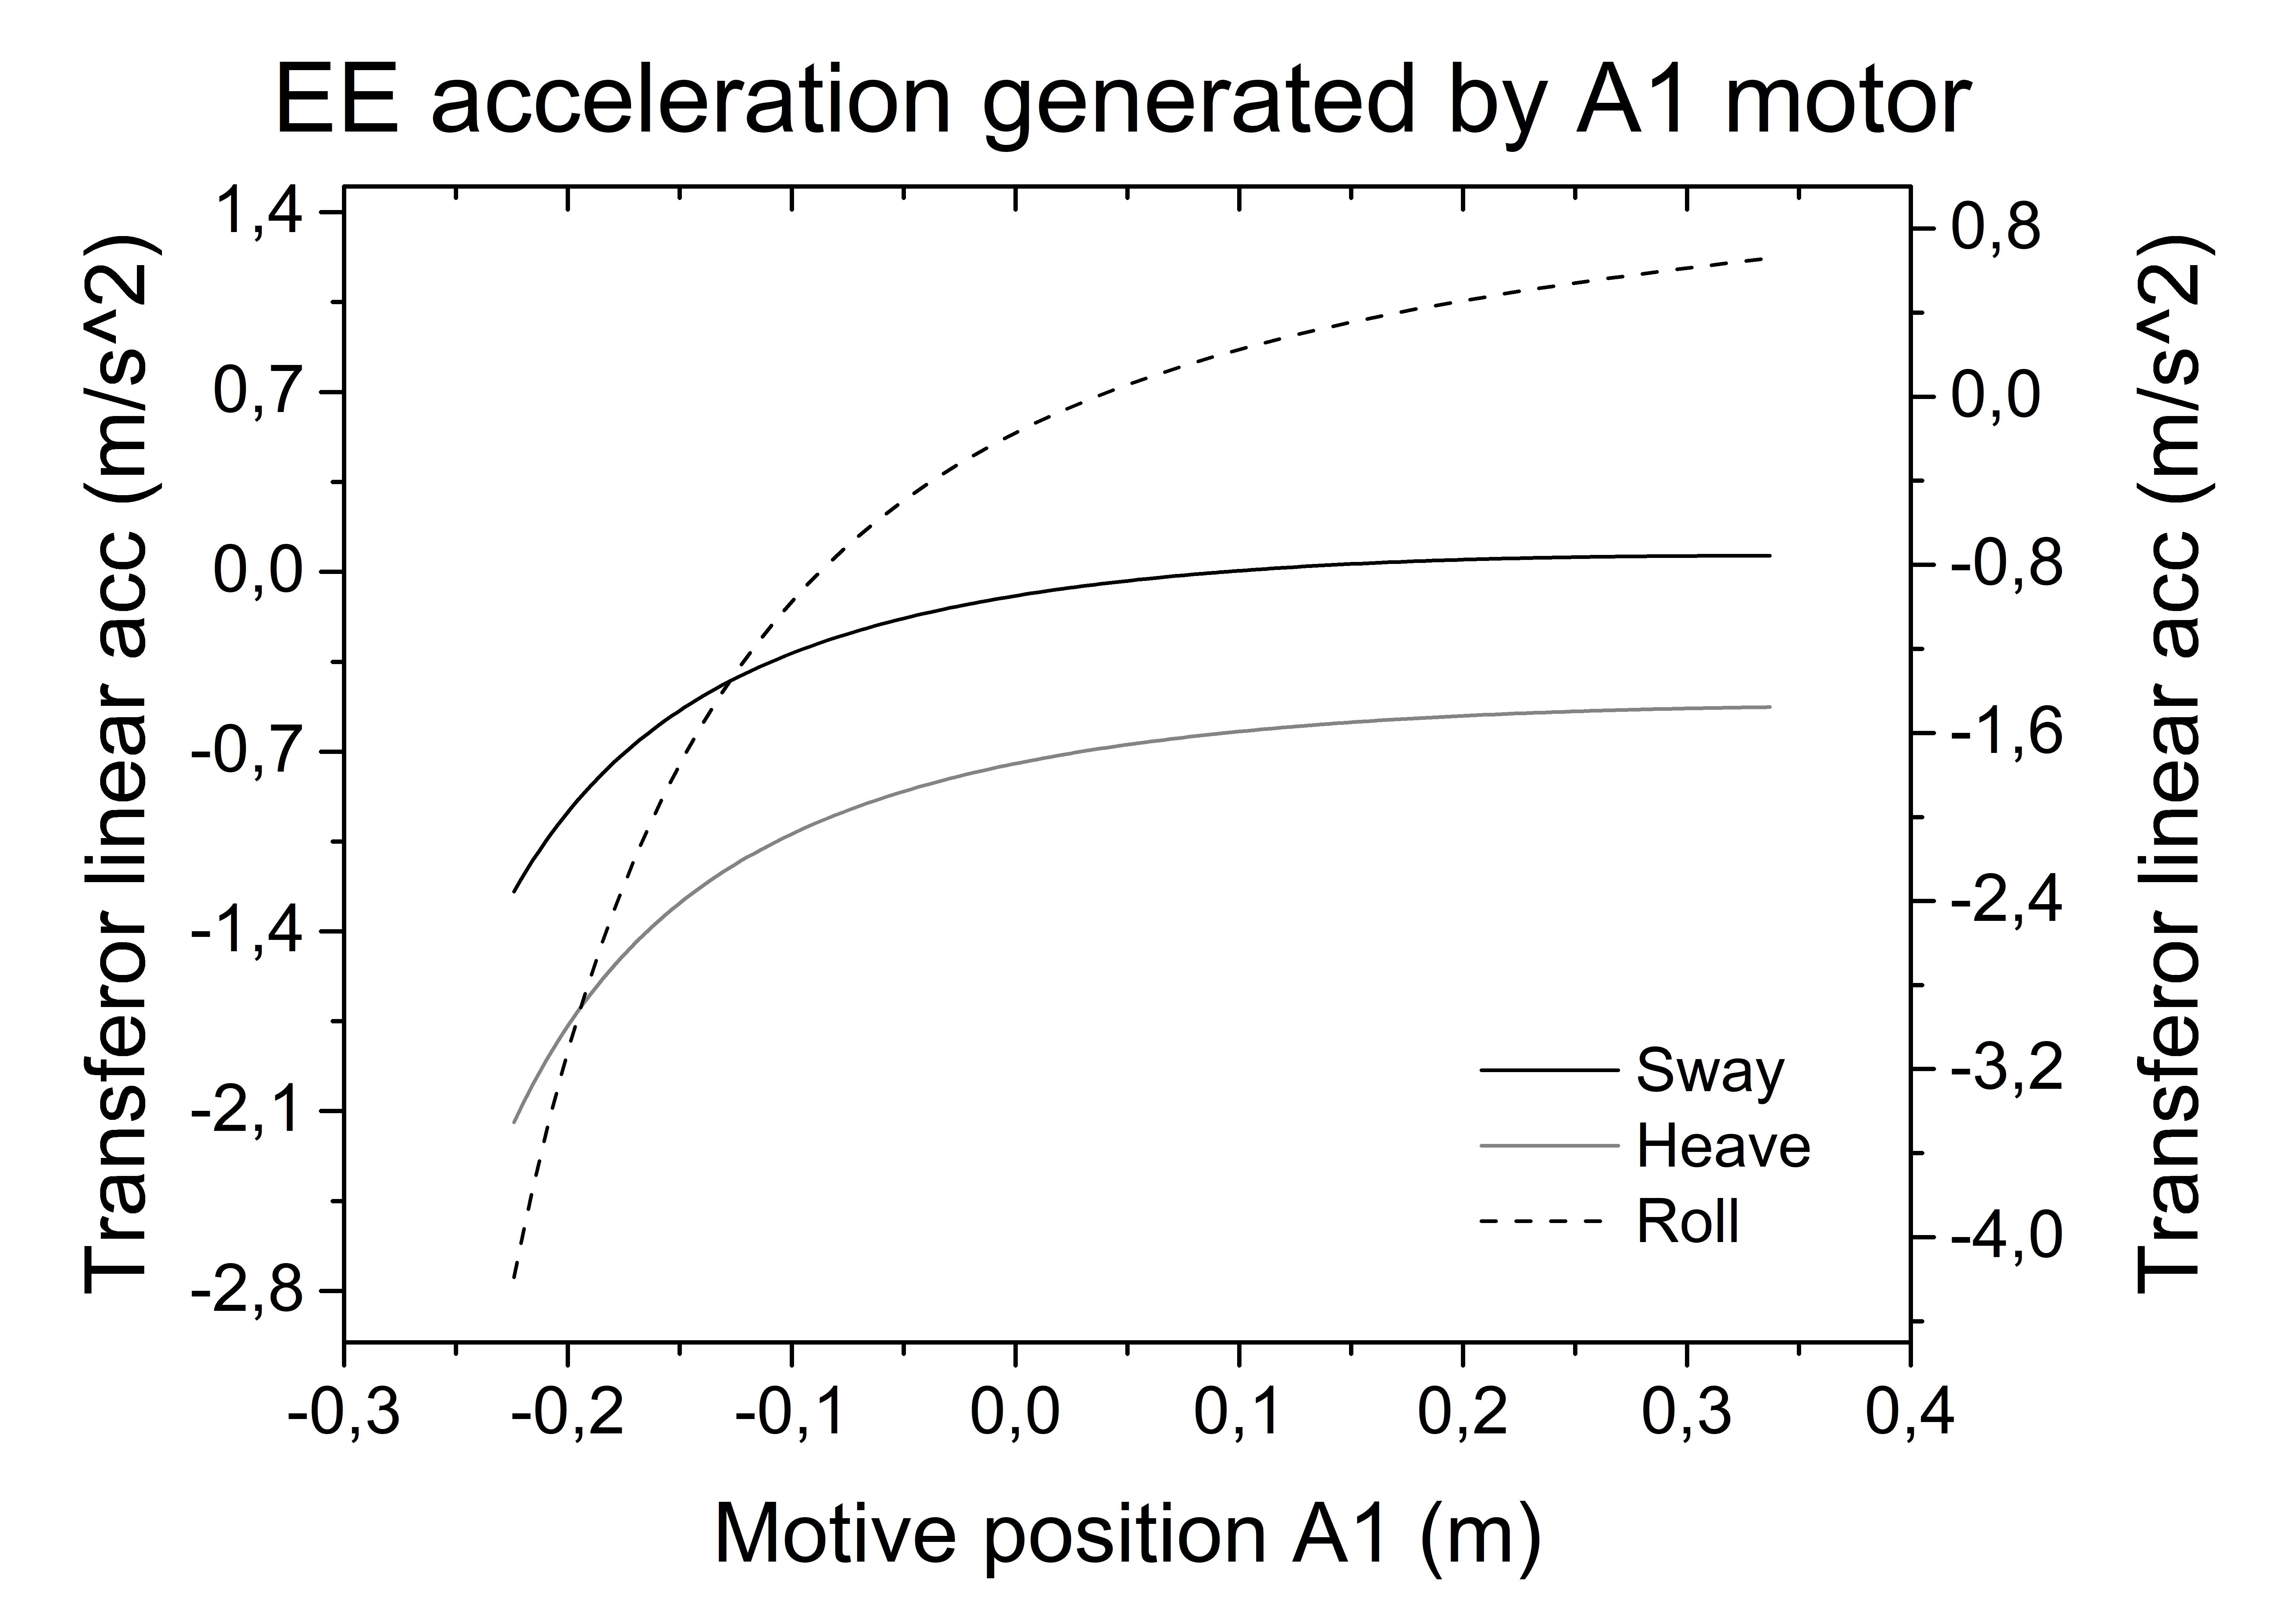
\includegraphics[width=7.5cm]{Images/EE_acc_A1}
	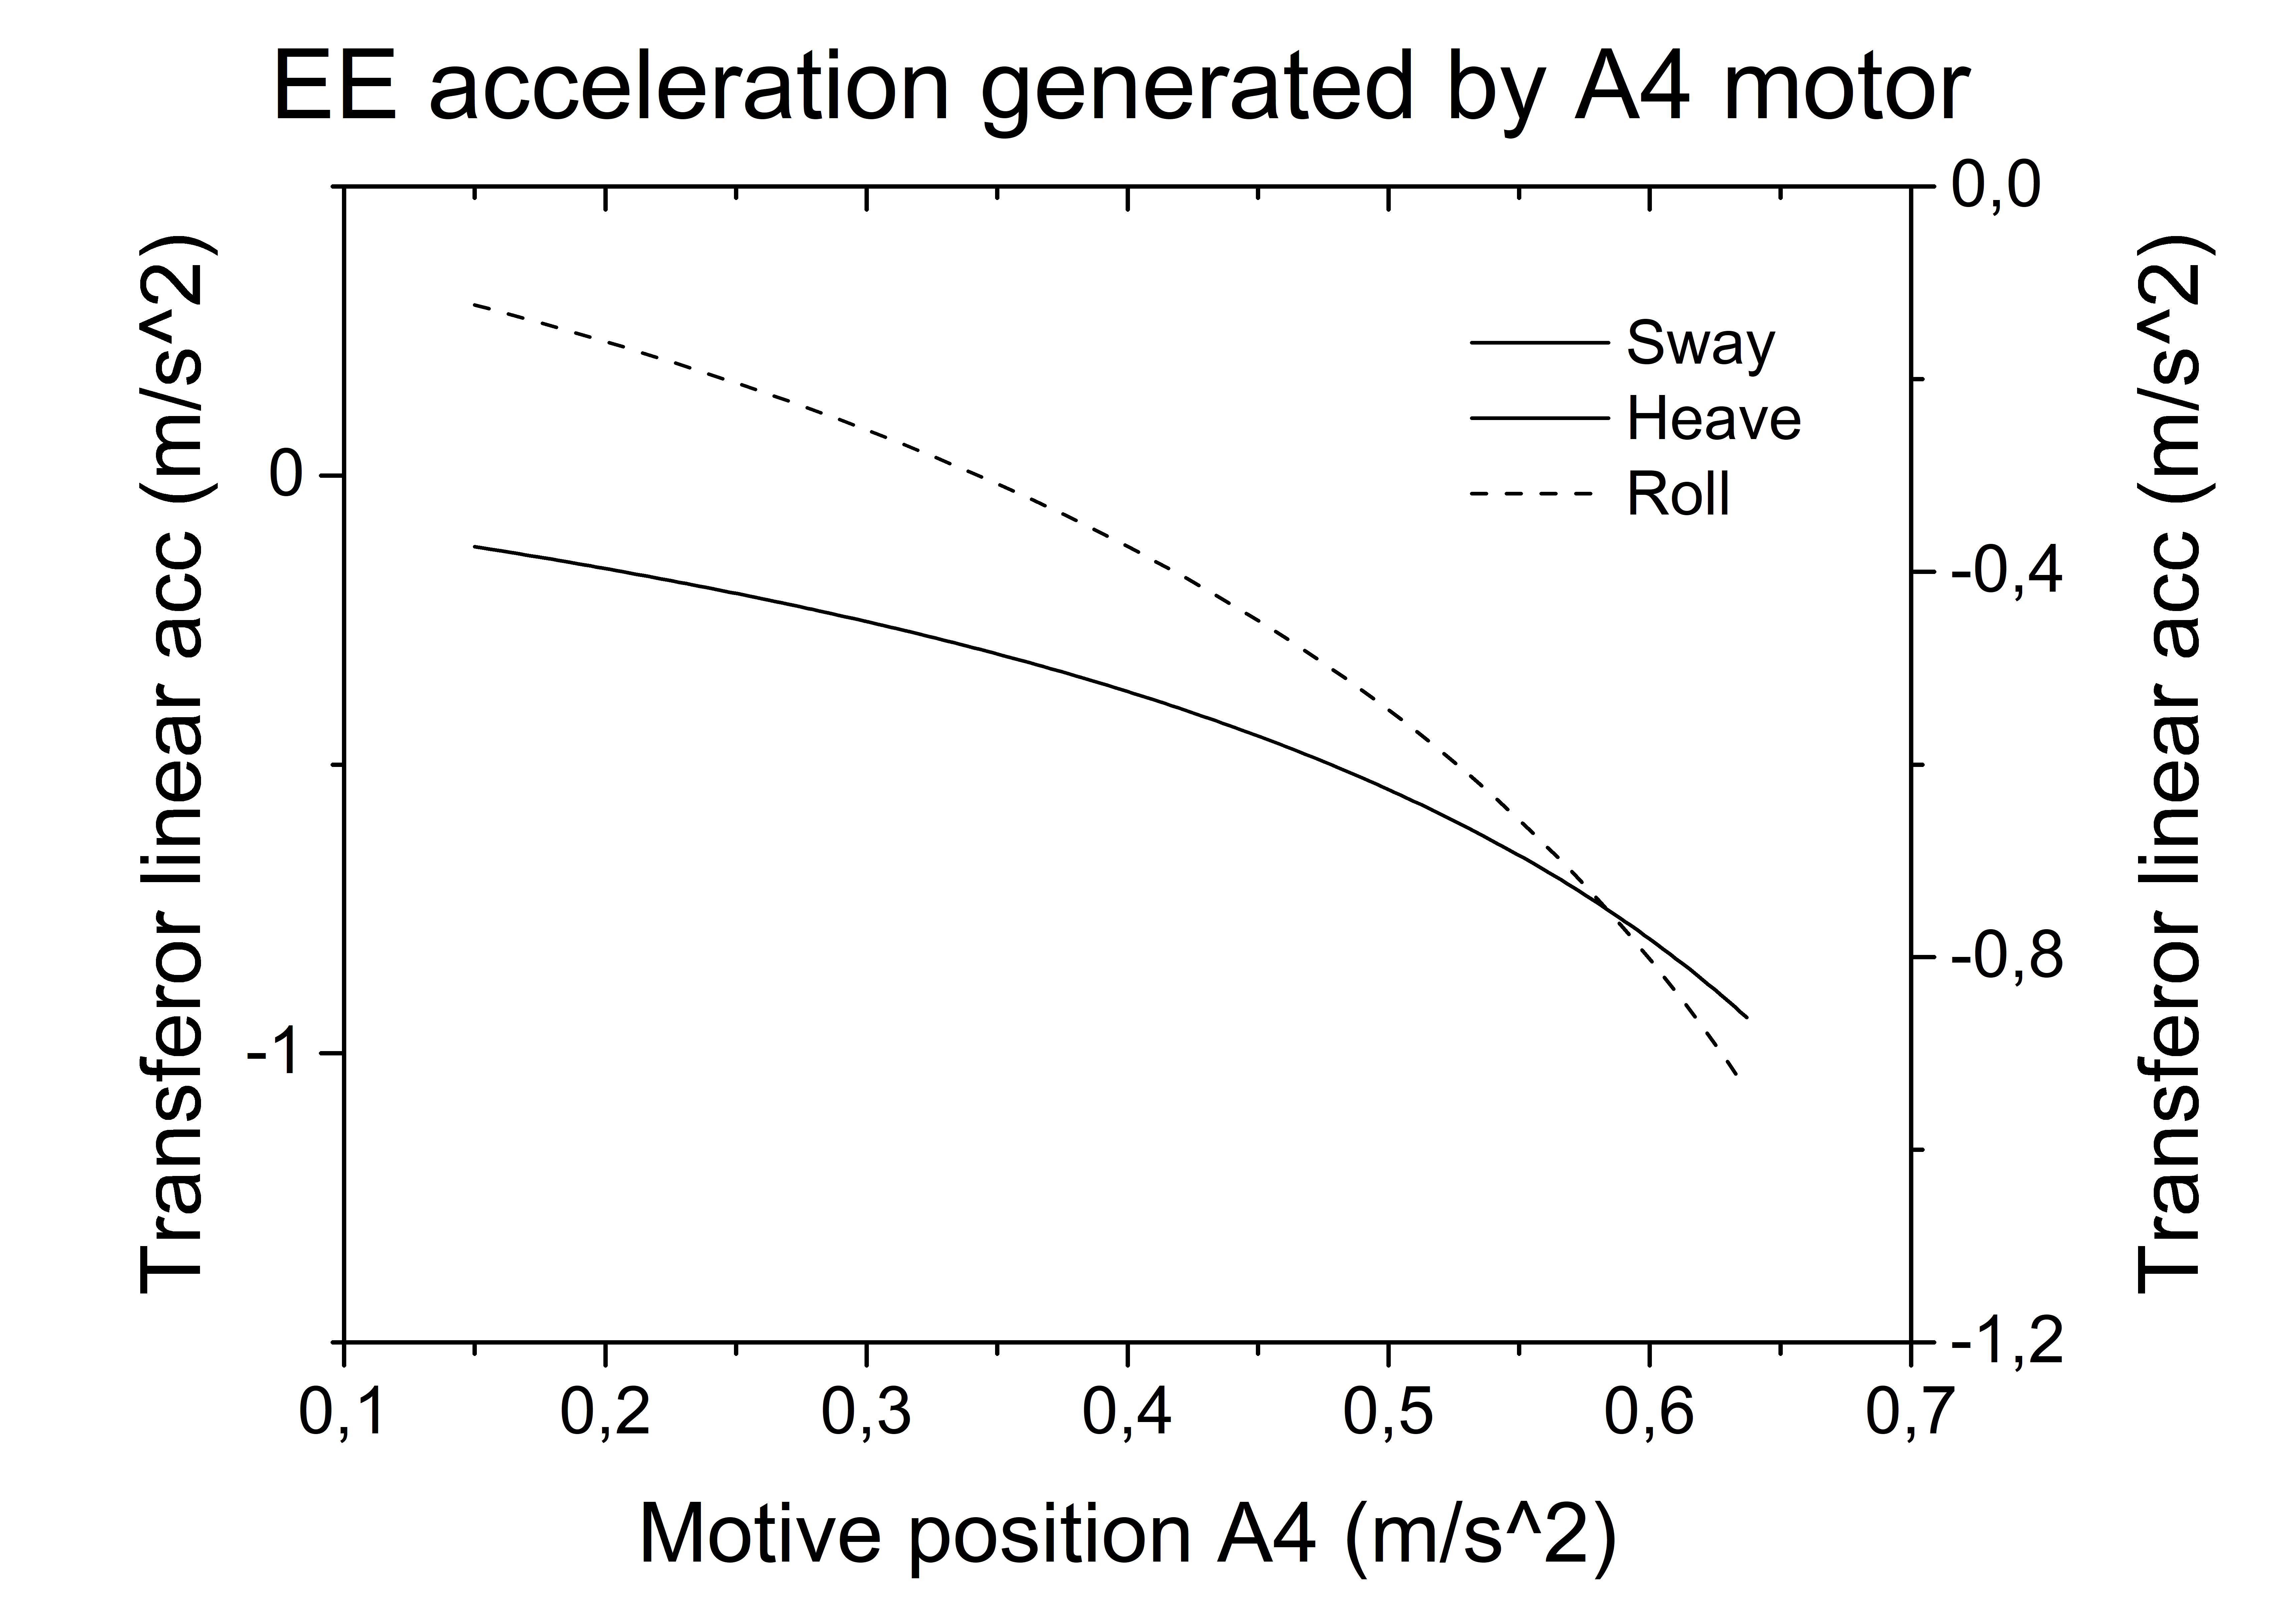
\includegraphics[width=7.5cm]{Images/EE_acc_A4}
	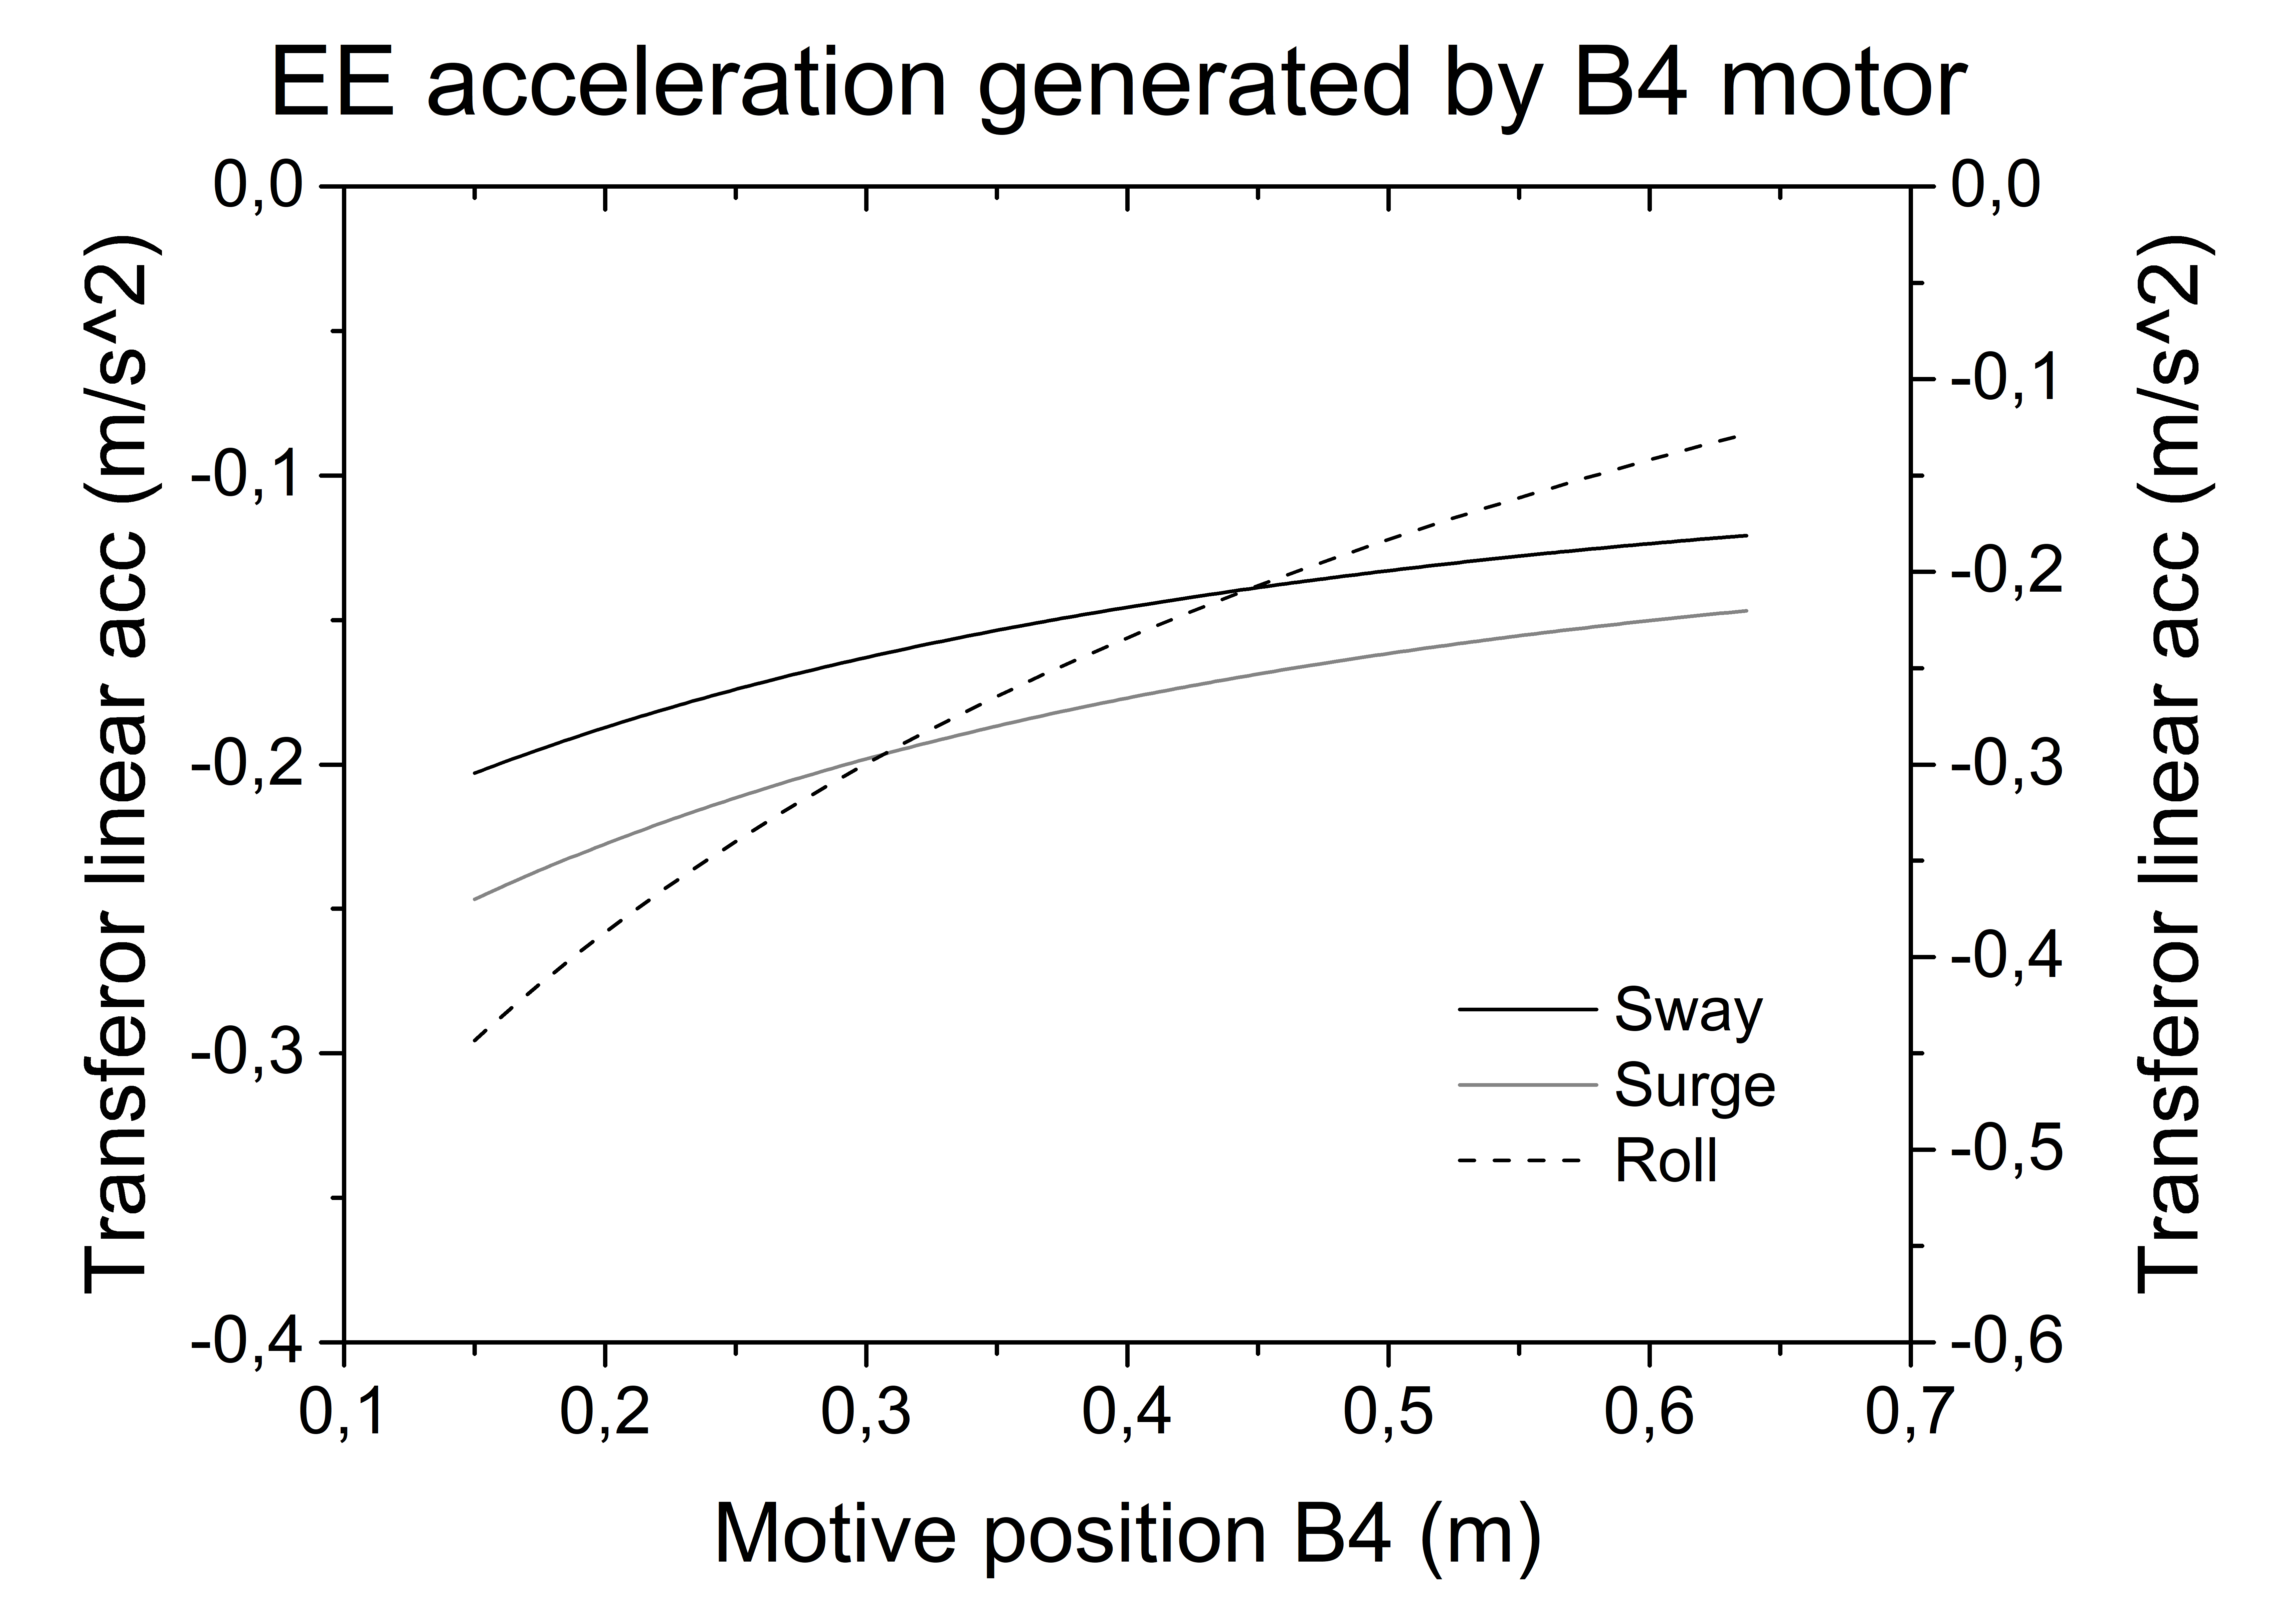
\includegraphics[width=7.5cm]{Images/EE_acc_B4}
	\caption{Accelerations of the end effector (\( EE \)) as a function of the motion positions.}
	\label{fig:acc}
\end{figure}

\section{Influence of the main design parameters}
\label{s:Parameters}
As shown in Section \ref{s:Position-workspaces}, by varying the position of the actuators it is possible to know which combinations of Sway - Heave - Roll can be reached by the end effector, i.e. the workspace.\\
The workspace is one of the main parameters analyzed during the design and modelling phase of the mechanism: in particular it is required to maximize it to reach the requirements.

The procedures described in \ref{s:Extreme-positions} and \ref{s:Position-workspaces} have been used to systematically compute the workspaces depending on the design parameters of the driving simulator which are \( L_1 \), \( H_1 \), \( L_2 \), \( H_2 \), \( L_4 \) and \( \alpha_4 \), as it can be seen in Figure \ref{f:Sub-Mechanism}.

The objective is to develop a method for the identification of the most important design parameters, i.e. the ones that influence the most the workspaces.

The main idea consists in varying one parameter at a time, assigning it to three different values, keeping the others equal to the following set:
\begin{itemize}
  \item \( L_1 = 0.25 m\);
  \item \( H_1 = 0.25 m\);
  \item \( L_2 = 1 m\);
  \item \( H_2 = 0.6 m\);
  \item \( L_4 = 0.7 m\);
  \item \( \alpha_4 = \pi/6\).
\end{itemize}

For each parameter, three different values were considered, as shown in Table \ref{tab:values}. Then it has been obtained a triplet of workspaces' clouds of points associated to the three different values, to explore the overall impact of a change in the design parameter on the resulting workspaces.

\begin{table}[h!]
    \centering
      \begin{tabular}{C{0.35cm}C{1.4cm}C{1.4cm}C{1.4cm}}
        & \textbf{Value 1} & \textbf{Value 2} & \textbf{Value 3} \\
        \\
        \hline
        \hline
        \\
        \(\alpha_{4}\) & \(\pi/9\) & \(\pi/6\) & \(\pi/5\) \\

        \(H_{1}\) & \(0.1\) & \(0.25\) & \(0.4\) \\

        \(H_{2}\) & \(0.4\) & \(0.6\) & \(0.8\) \\

        \(L_{2}\) & \(0.8\) & \(1\) & \(1.2\) \\

        \(L_{4}\) & \(0.5\) & \(0.7\) & \(0.9\) \\
        \\
        \hline
      \end{tabular}
    \caption{caption}
    \label{tab:values}
  \end{table}

Furthermore, data were exported and analyzed in \textsc{Matlab}\textsuperscript{TM}, exploiting its numeric effectiveness. Using the \texttt{boundary} command, the border of each workspace has been extracted, togheter with the numeric values of its area. The area's value is particularly useful because it leads to a solid criterion, based on numeric values, for the identification of the most impactful design parameter.

Observing the various obtained workspaces of Figures \ref{fig:ws_1}, \ref{fig:ws_2}, \ref{fig:ws_3} and \ref{fig:ws_4} it can be observed that:
\begin{itemize}
	\item there exist workspaces that satisfy the targets defined in the paper \textit{\Virgolette{System requirements}} for the Sway (\(0.65 m\)) and for the Roll (\(0.52 rad\));
	\item none of the workspaces is capable of realizing the Sway target of \(0.65 m\), implying a possible redefinition of it;
	\item increasing the value of the runner's inclination \(\alpha_4\) implies pushing down the \(x-y\) workspace;
	\item increasing the value of the \(H_2\) heigth implies pushing up the \(x-y\) workspace;
	\item changing the rod length \(L_2\) has high consequences on the three workspaces when going from \(L_2=0.8 m\) to \(1m\), but above this value the effectiveness is sort of \Virgolette{saturated} and changes are little.
\end{itemize}

For each design parameter, three values of areas have been computed, for each workspace. The reasoning behind the definition of the most influencing coefficients starts with the definition of the percentage change in the area:
\begin{equation}
  \label{e:areas}
  \Delta A_{\%} = \frac{A_{max} - A_{min}}{A_{min}}
\end{equation}
Also the percentage change of the specific parameter is defined as:
 \begin{equation}
   \label{e:params}
   \Delta param_{\%} = \frac{param_{max} - param_{min}}{param_{min}}
 \end{equation}
The \textit{influence indices} are defined as the ratio between \eqref{e:areas} and \eqref{e:params}, representing how much the area of the workspace increases in percentage as function of the percentage change of the design parameter:
  \begin{equation}
    \label{e:indices}
    i = \frac{\Delta A_{\%}}{\Delta param_{\%}}
  \end{equation}

Parameters that involve higher influence indeces are the most promising for the optimization of the driving simulator mechanism's workspace.
All the results are summed up in Table \ref{tab:indeces}.

\begin{table}[h!]
    \centering
      \begin{tabular}{C{0.5cm}C{0.90cm}C{0.90cm}C{0.90cm}C{1.10cm}}
        & \(i_{x-y}\) & \(i_{x-roll}\) & \(i_{y-roll}\) & \(i_{x-y-roll}\) \\
        \\
        \hline
        \hline
        \\
        \(\alpha_{4}\) & \(1.58\) & \(0.58\) & \(2.77\) & \(1.79\) \\

        \(H_{1}\) & \(0.16\) & \(0.08\) & \(0.12\) & \(0.32\) \\

        \(H_{2}\) & \(0.29\) & \(0.09\) & \(0.21\) & \(0.14\) \\

        \(L_{2}\) & \(0.95\) & \(0.97\) & \(0.92\) & \(2.07\) \\

        \(L_{4}\) & \(1.38\) & \(1.26\) & \(1.93\) & \(2.39\) \\
        \\
        \hline
      \end{tabular}
    \caption{caption}
    \label{tab:indeces}
  \end{table}

Concluding, the most effective design parameters are the runner's inclination \(\alpha_4\), the runner's stroke (indirectly represented by \(L_4\)) and the rod length \(L_2\).

\section{Future works}
The kinematics analysis developed in this paper plays a key role in the modelling process of the driving simulator mechanism, giving a lot of useful information for a well thought design.

Future works should involve the investigation of a large amount of possible combinations of design parameters, using the automatic procedures developed so far to compute workspaces, velocities and accelerations. Precisely for the fact that the entire process is symbolic and automatic, an optimization algorithm can be developed, in order to obtain the design parameters. The cost function could be, for example, the area of the workspaces or their shape.

Another important step of the analysis could be the 3D model of the entire mechanism, with the application of the crucial steps illustrated in this paper to the other planes.

Moreover, a dynamic analysis of the system must be performed.

\newgeometry{left=1.7cm,right=1.7cm,top=2.7cm,bottom=2.7cm}
\begin{figure*}
\centering
\begin{minipage}{0.49\textwidth}
	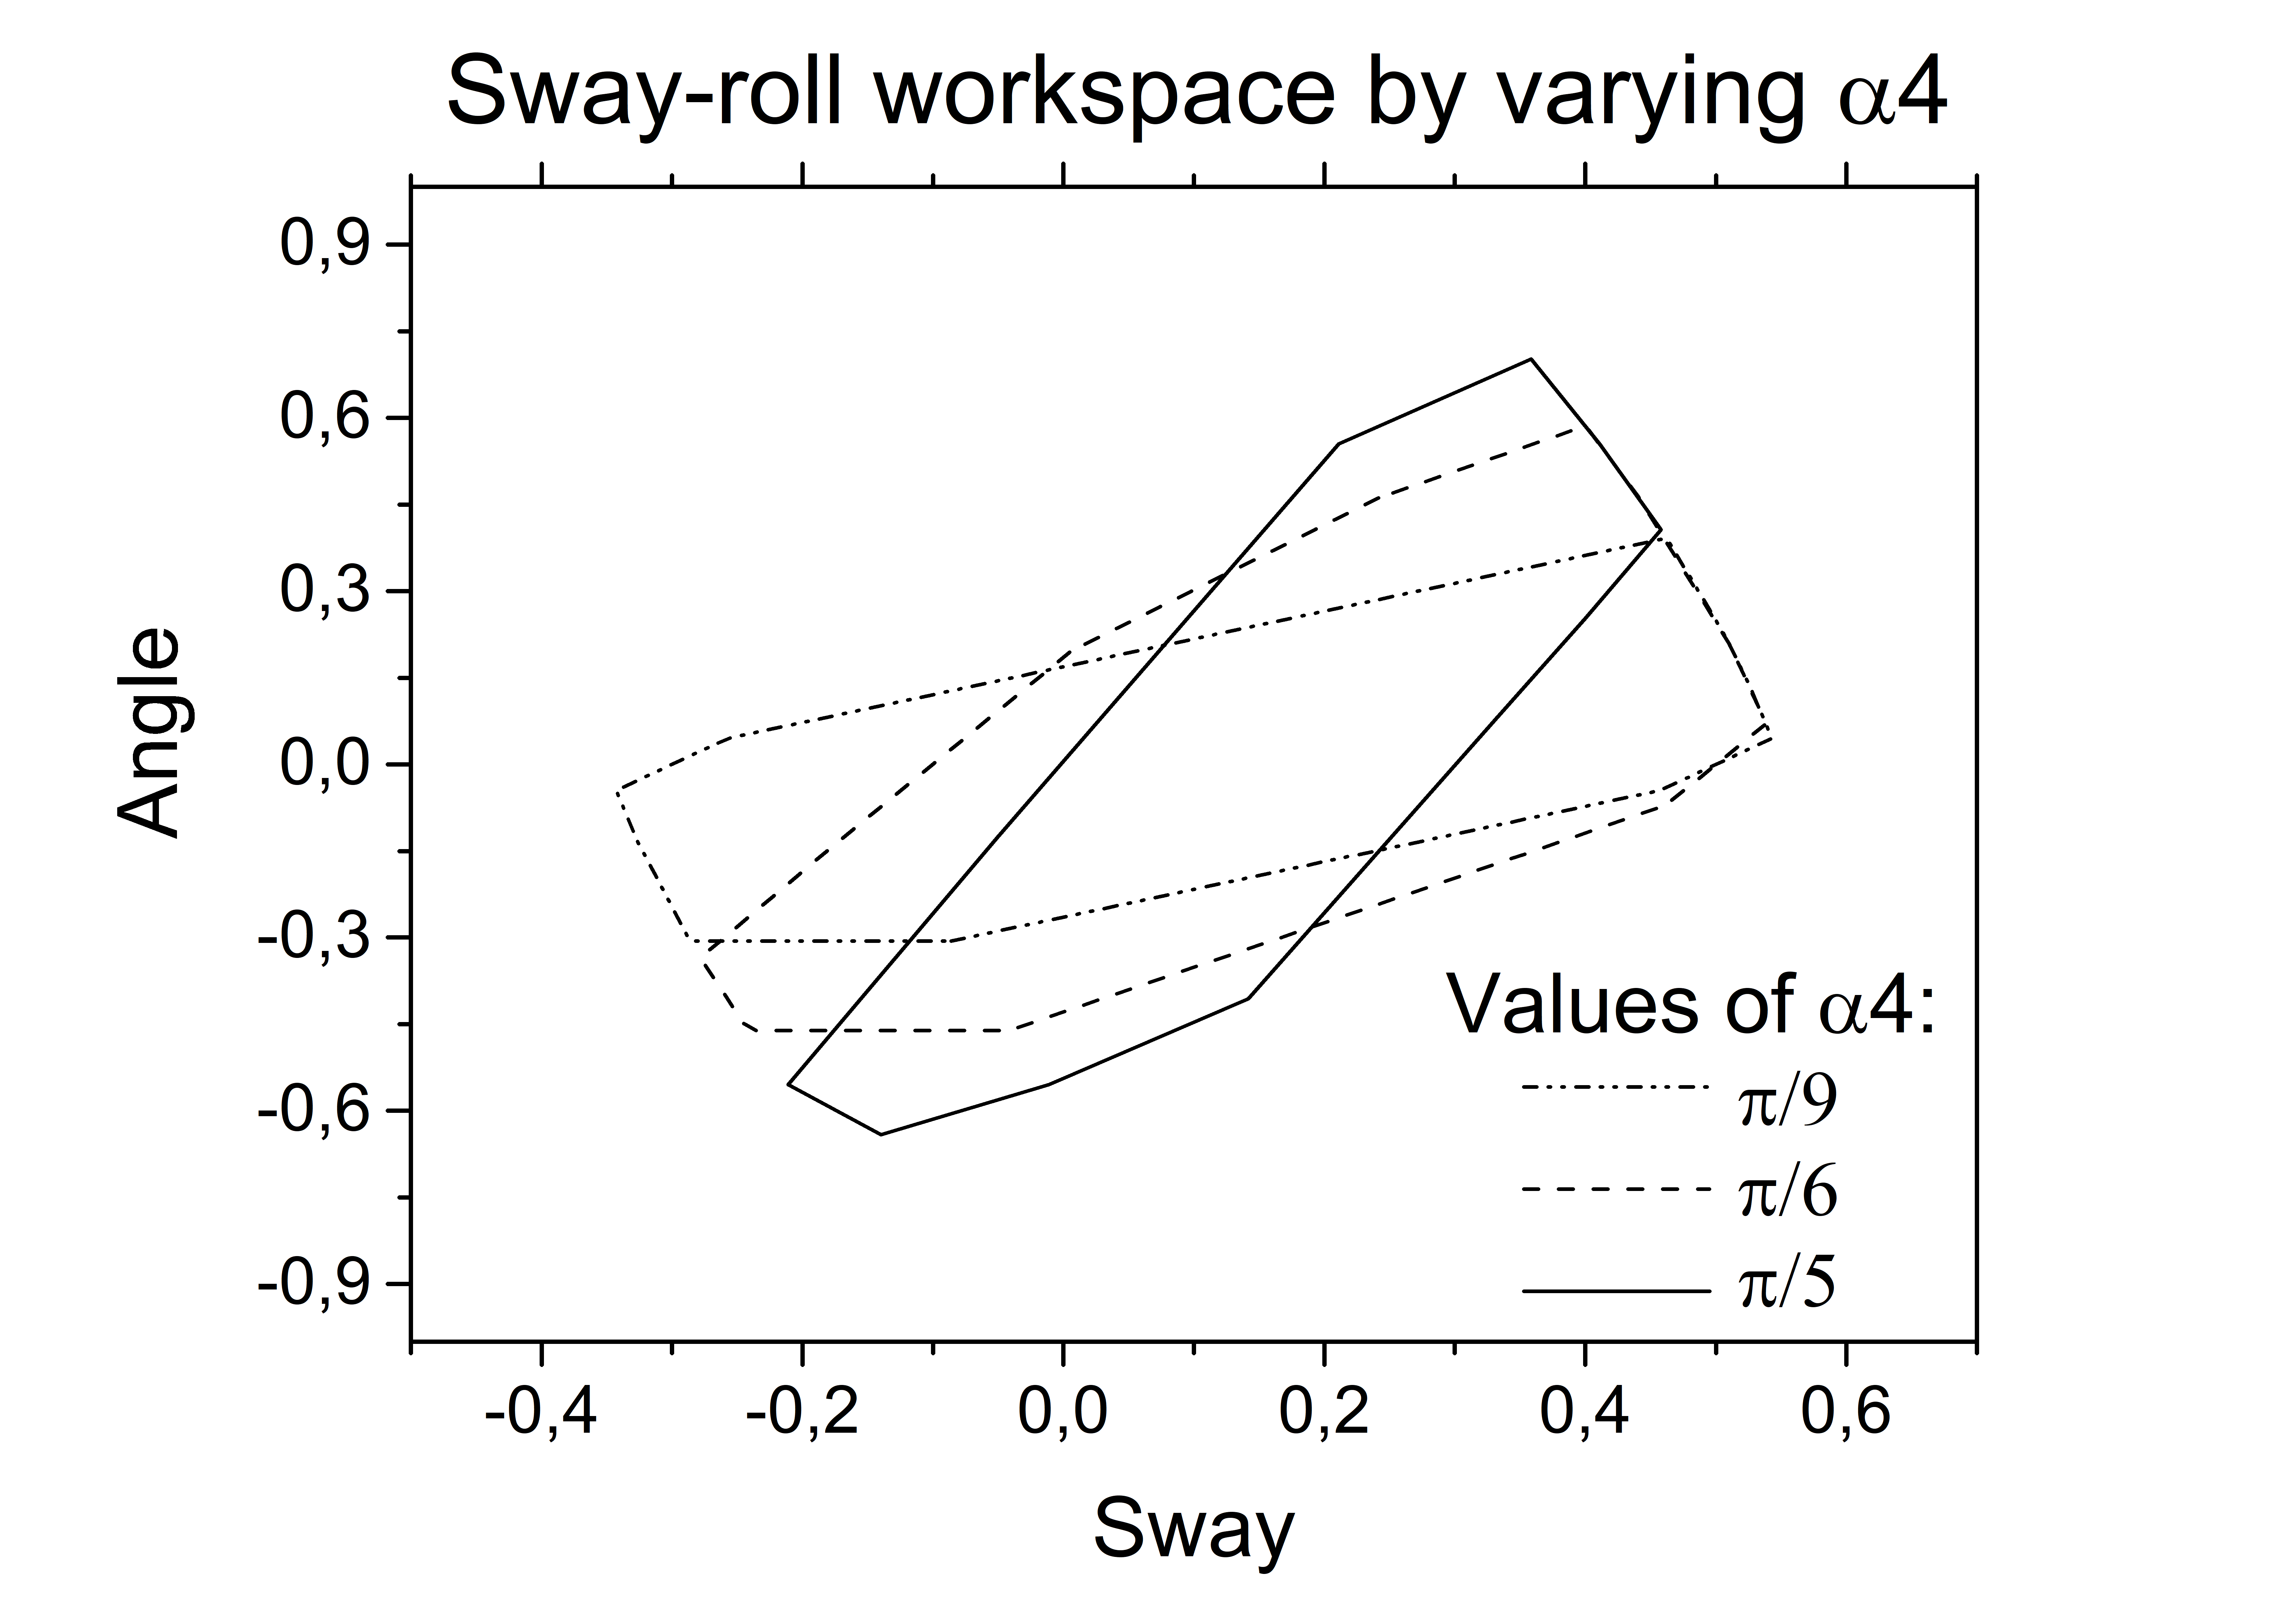
\includegraphics[width=7.5cm]{Images/ws_a4_xa}
\end{minipage}
\begin{minipage}{0.49\textwidth}
	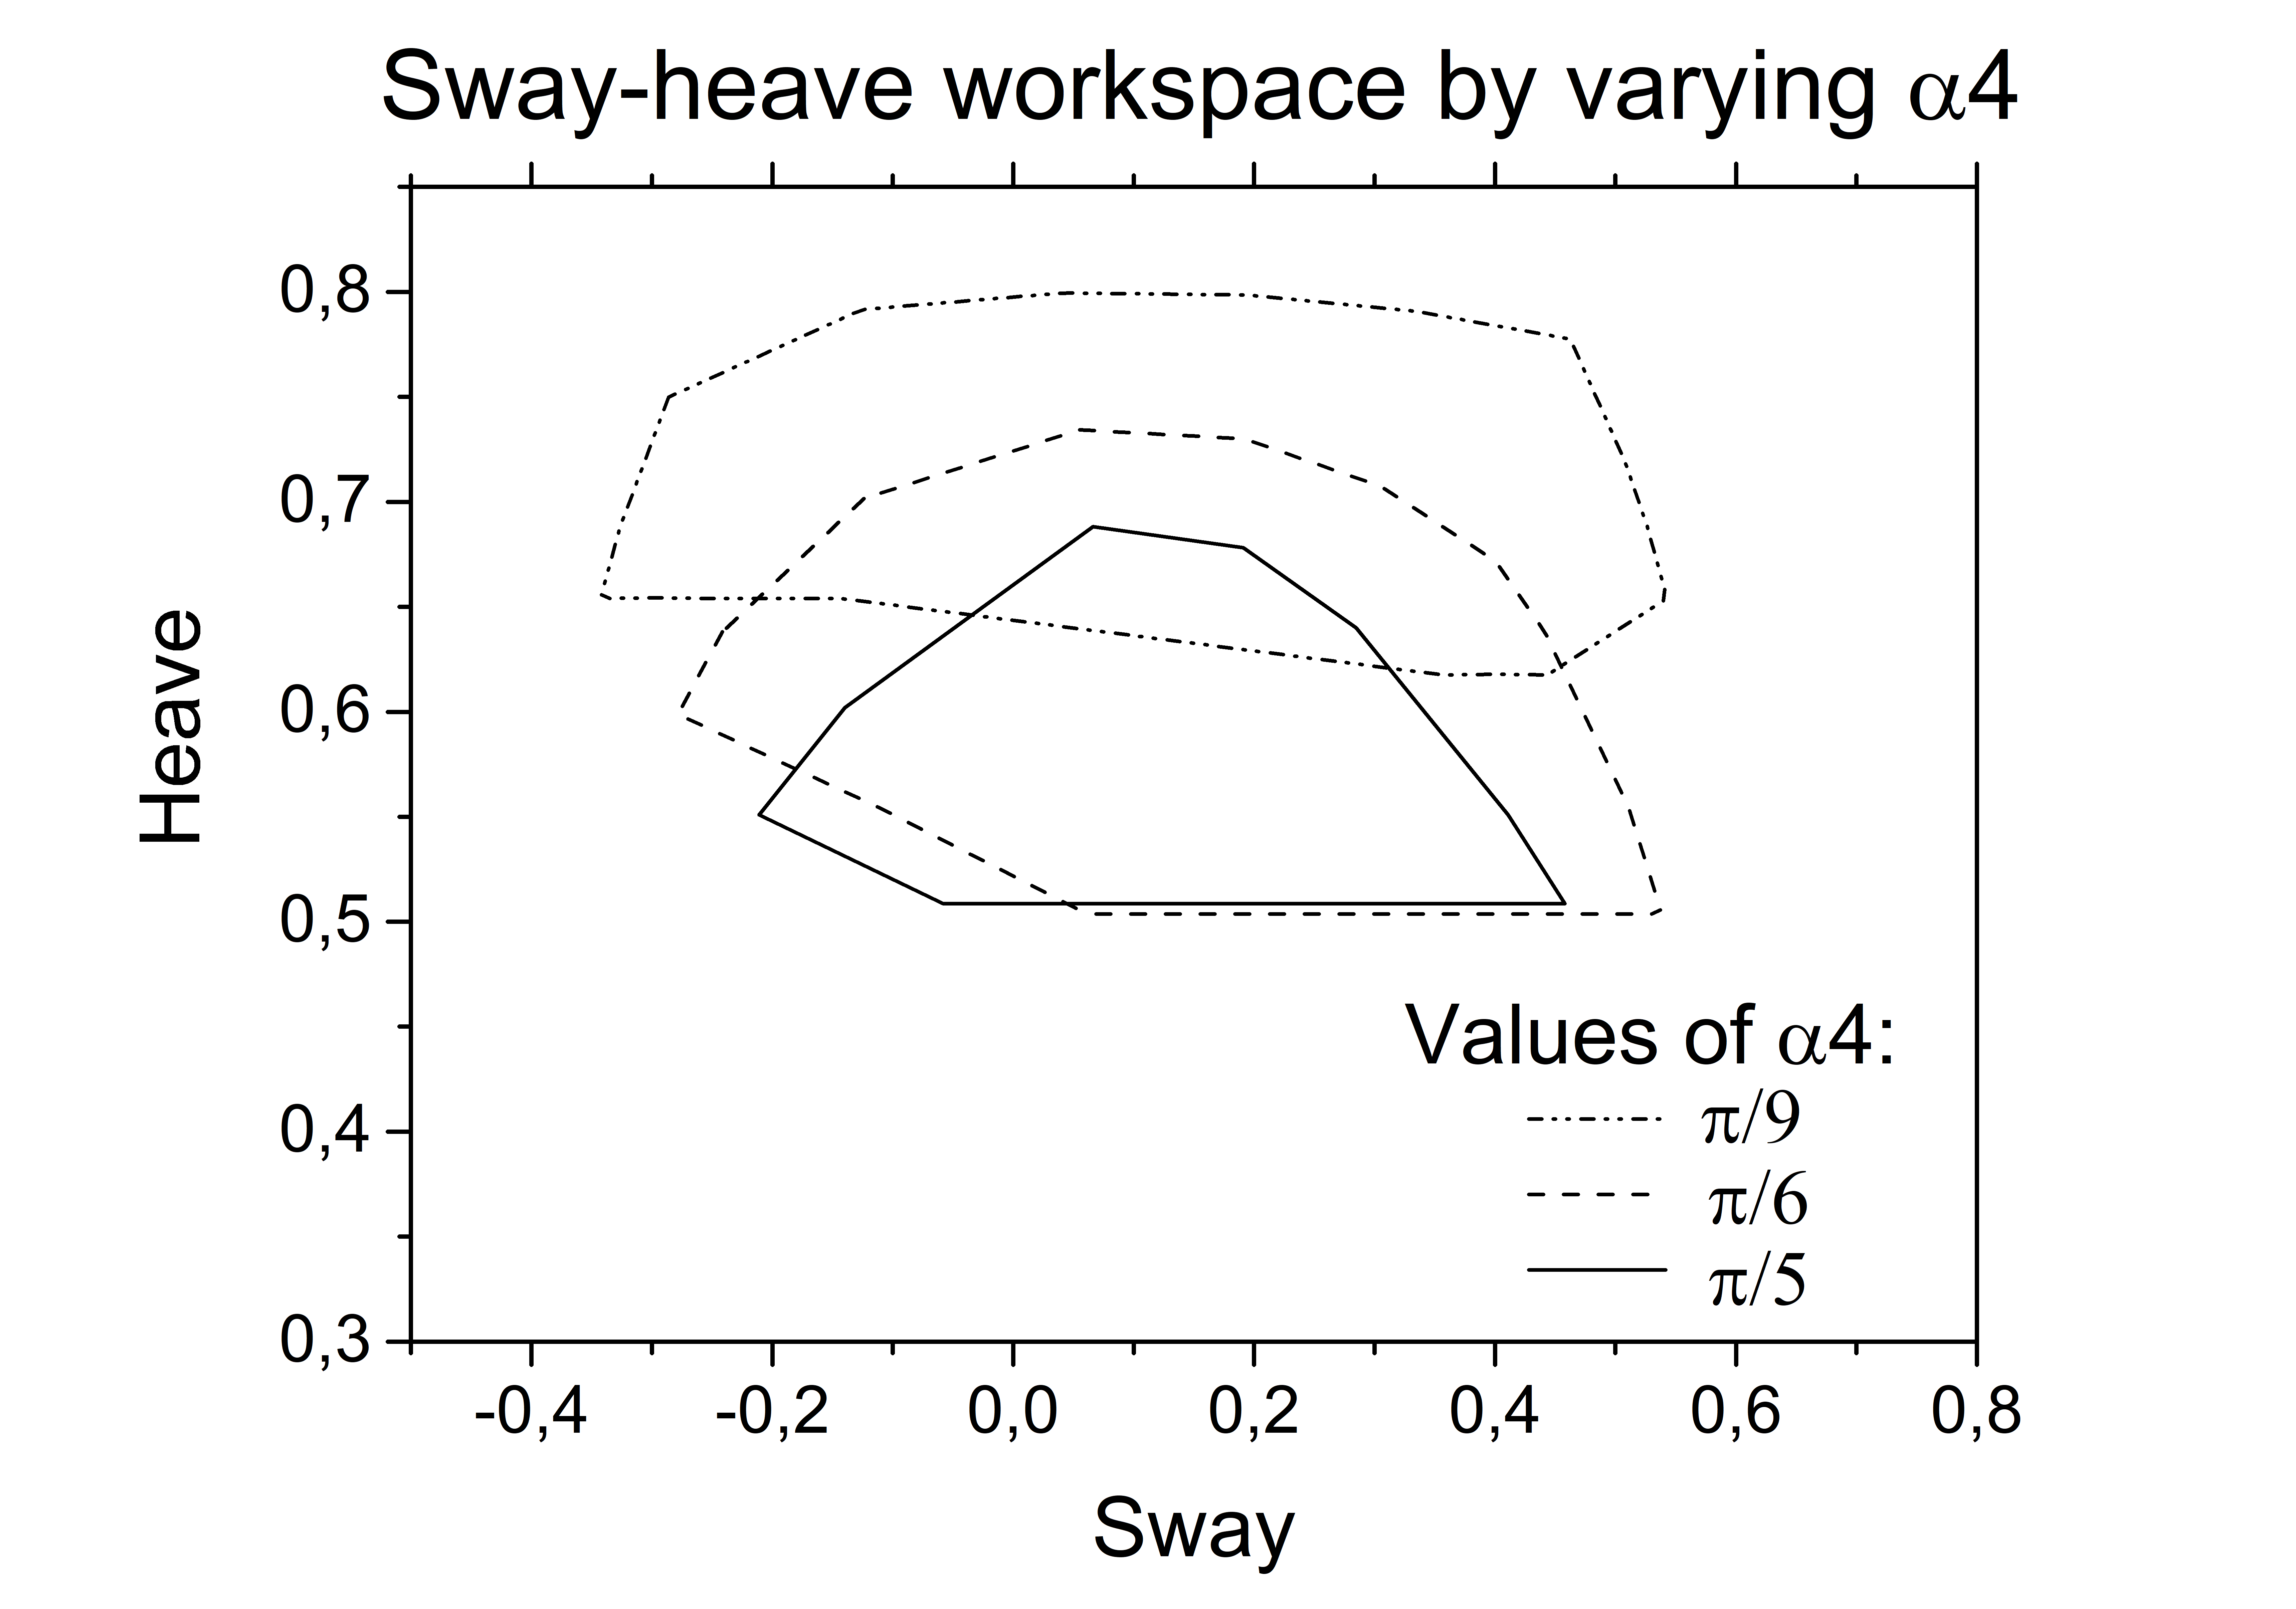
\includegraphics[width=7.5cm]{Images/ws_a4_xy}
\end{minipage}
\begin{minipage}{0.49\textwidth}
	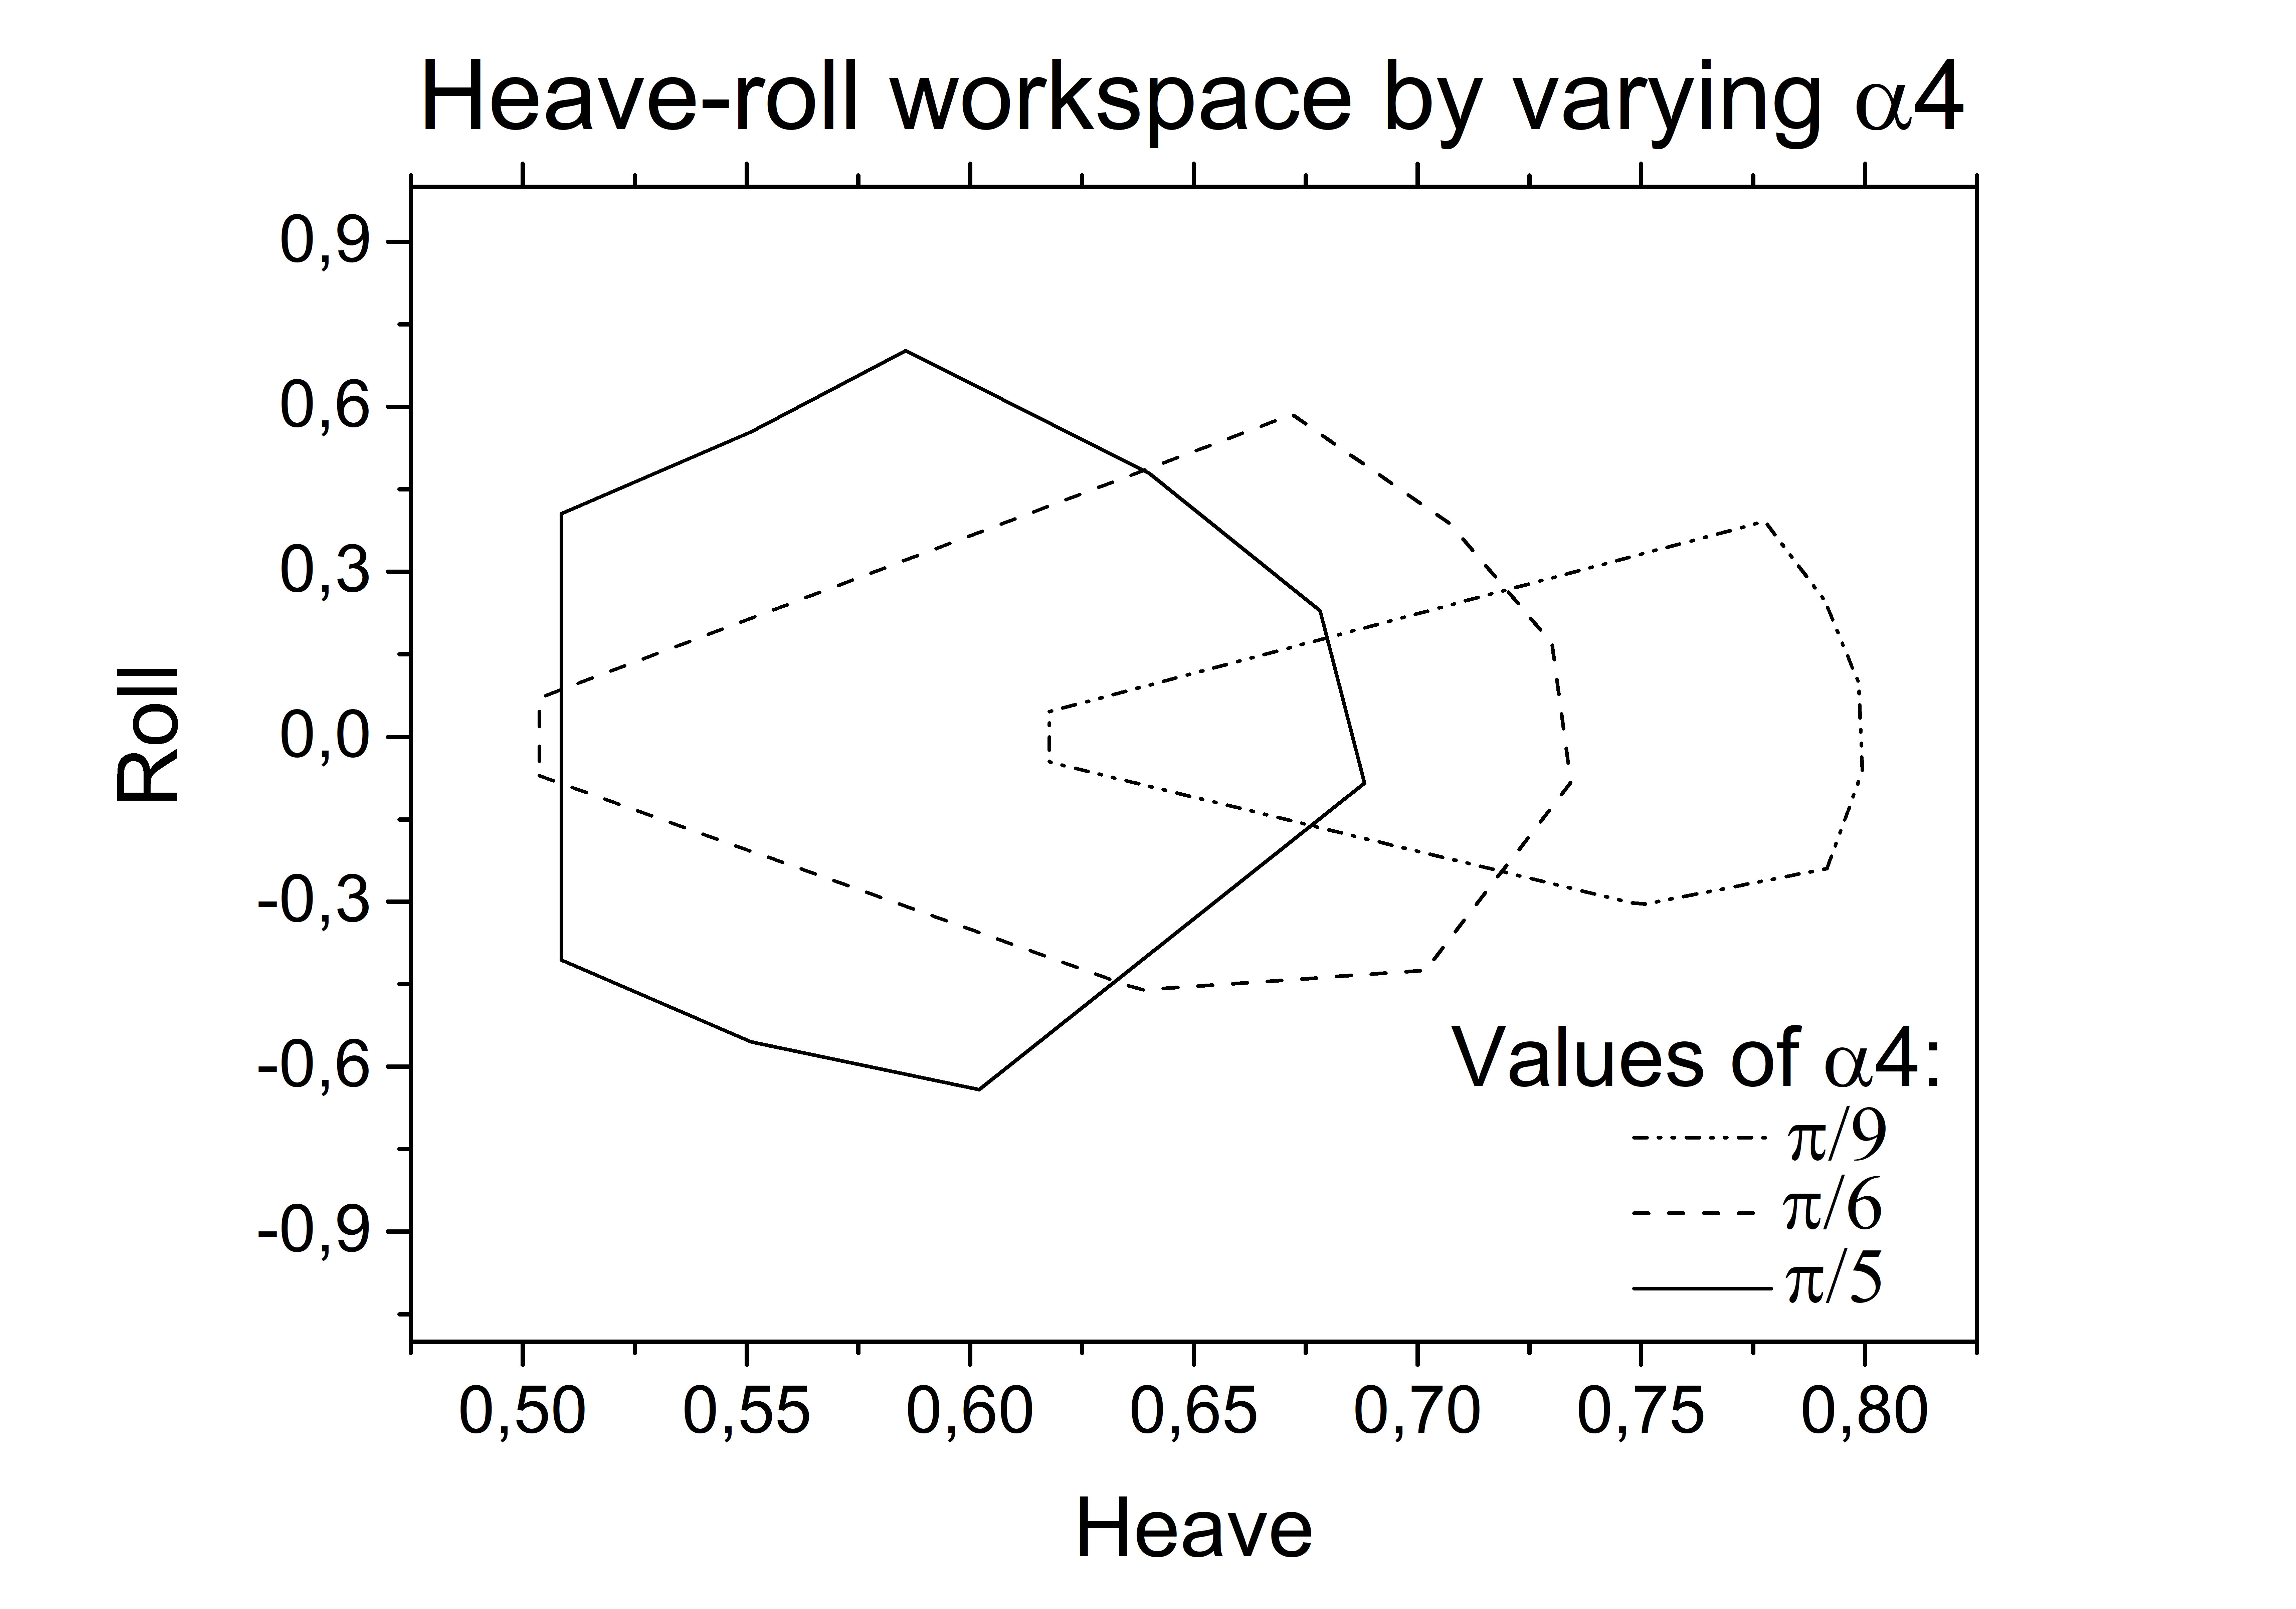
\includegraphics[width=7.5cm]{Images/ws_a4_ya}
\end{minipage}
    \caption{Variation of the workspace as a function of \( \alpha_4 \).}
    \label{fig:ws_1}
\end{figure*}

\begin{figure*}
\centering
\begin{minipage}{0.49\textwidth}
	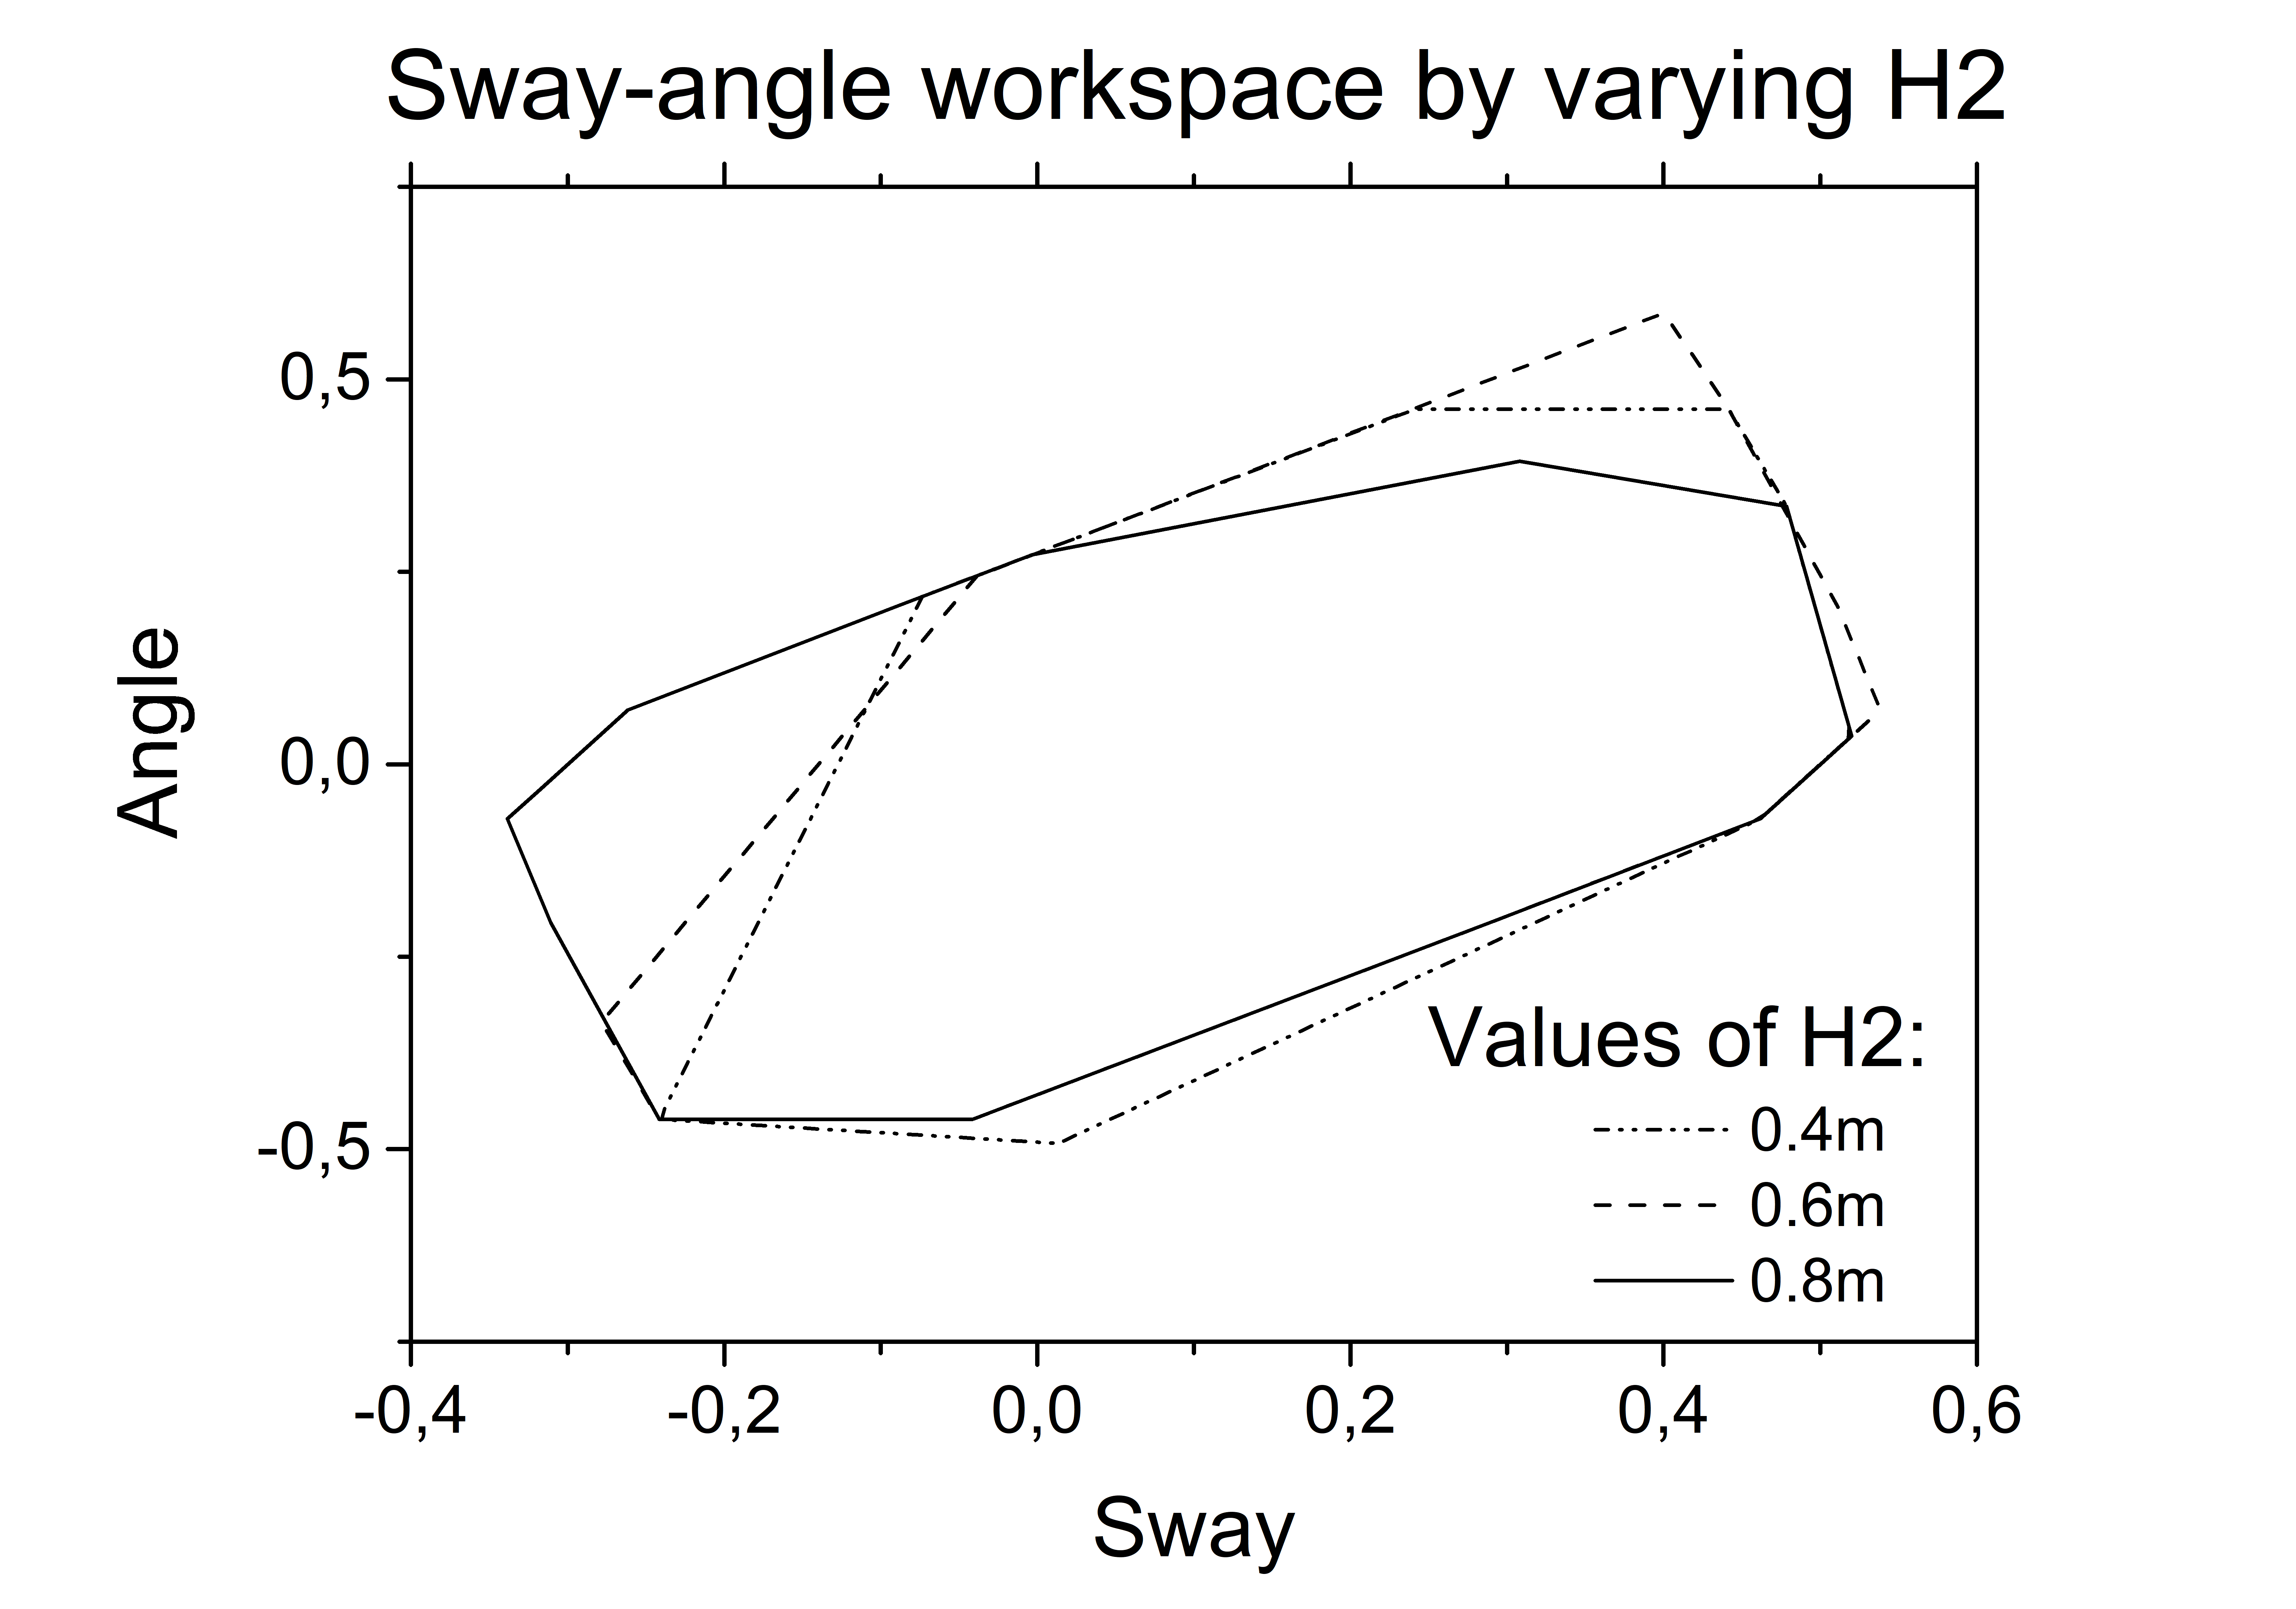
\includegraphics[width=7.5cm]{Images/ws_h2_xa}
\end{minipage}
\begin{minipage}{0.49\textwidth}
	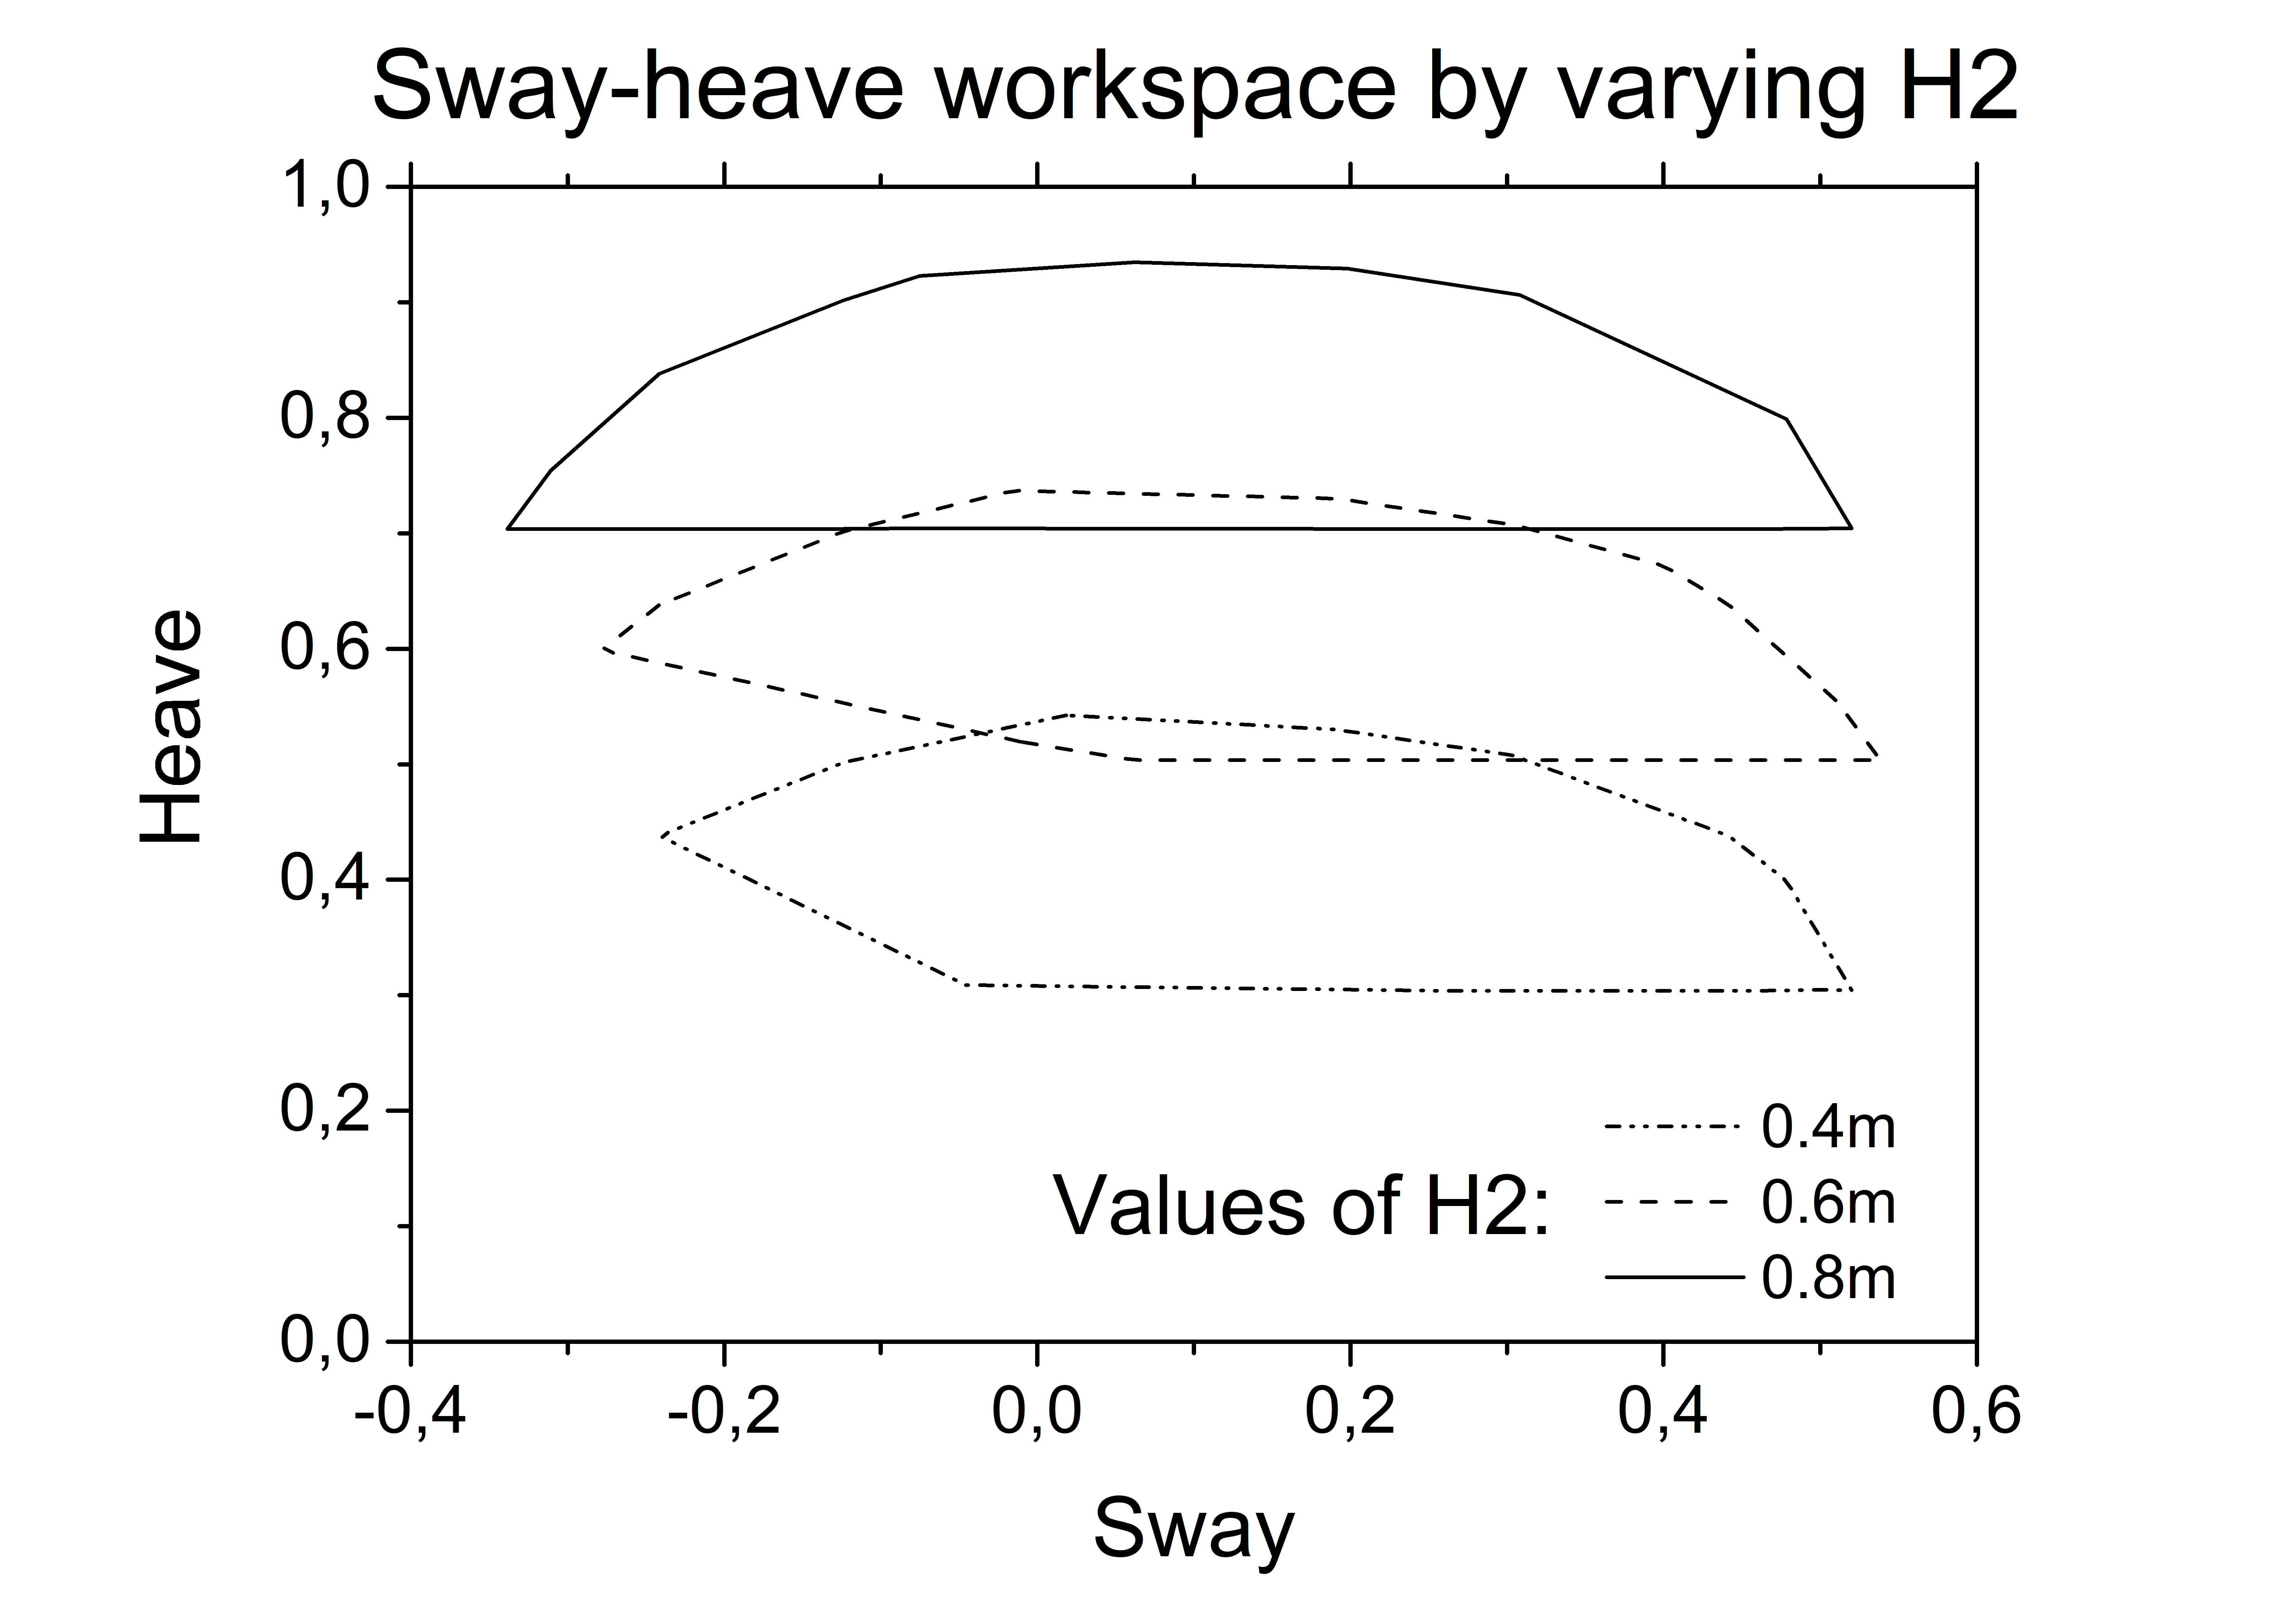
\includegraphics[width=7.5cm]{Images/ws_h2_xy}
\end{minipage}
\begin{minipage}{0.49\textwidth}
	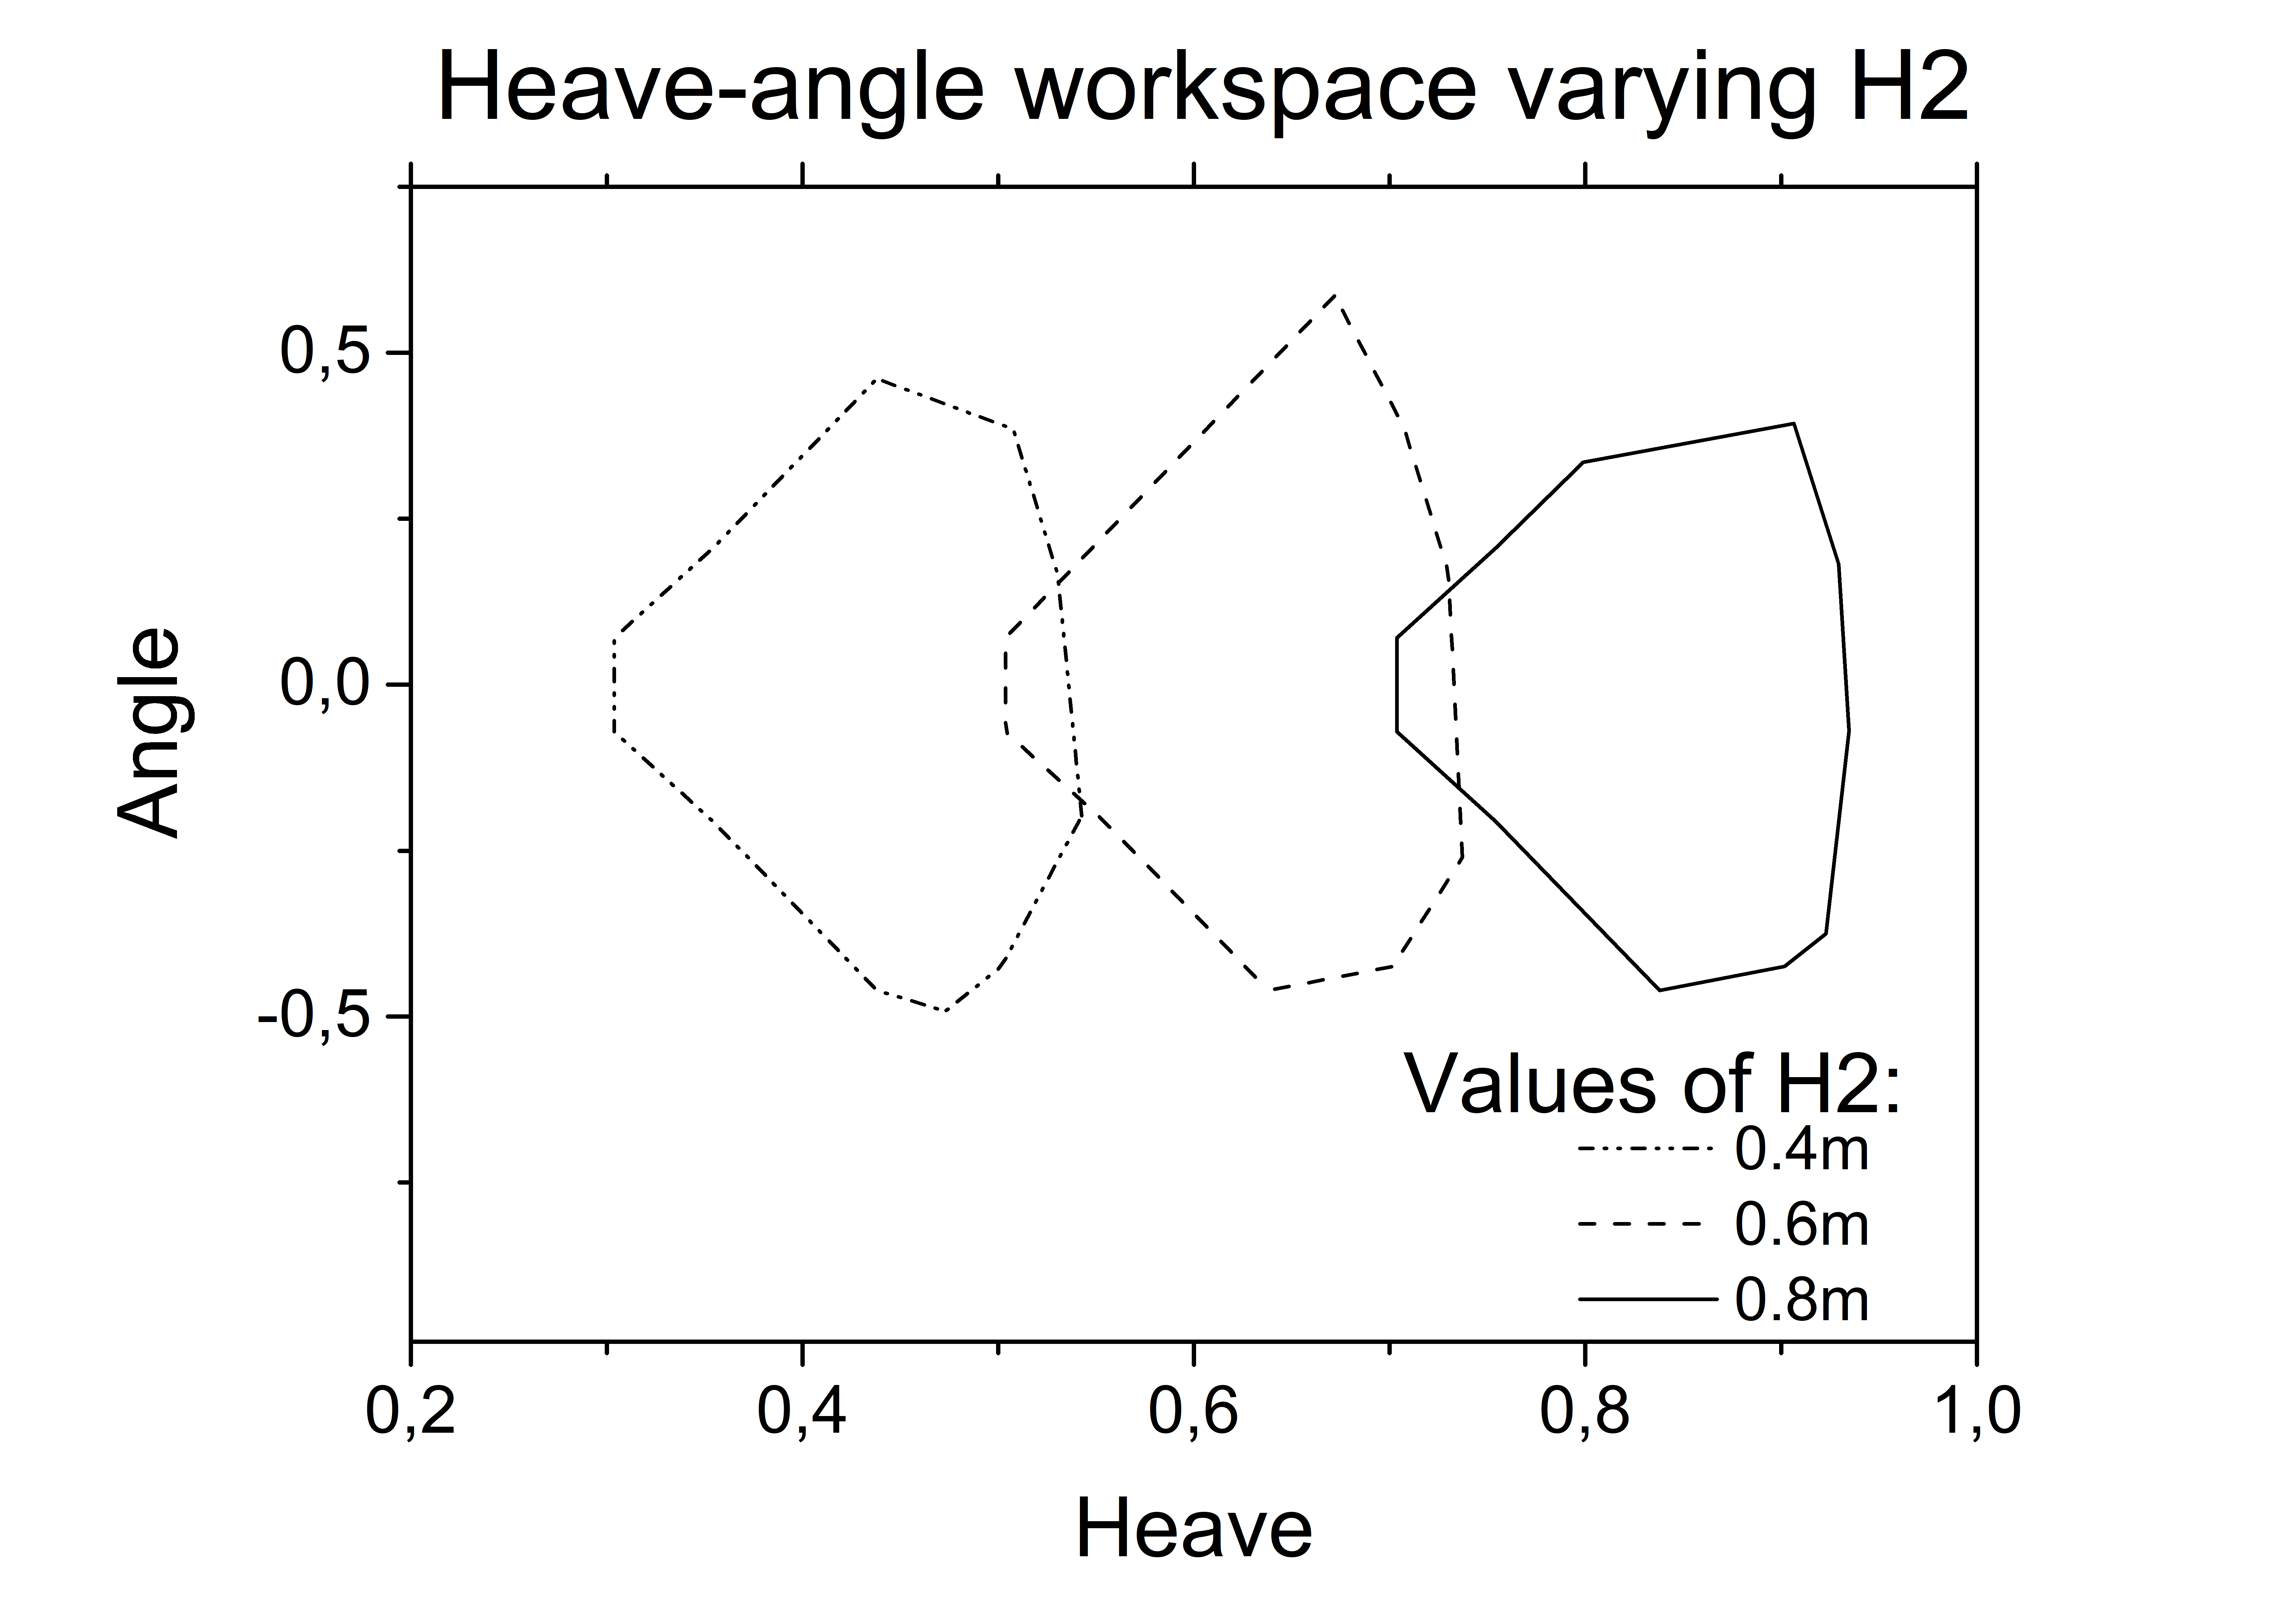
\includegraphics[width=7.5cm]{Images/ws_h2_ya}
\end{minipage}
    \caption{Variation of the workspace as a function of \( H_2 \).}
    \label{fig:ws_2}
\end{figure*}

\begin{figure*}
\centering
\begin{minipage}{0.49\textwidth}
	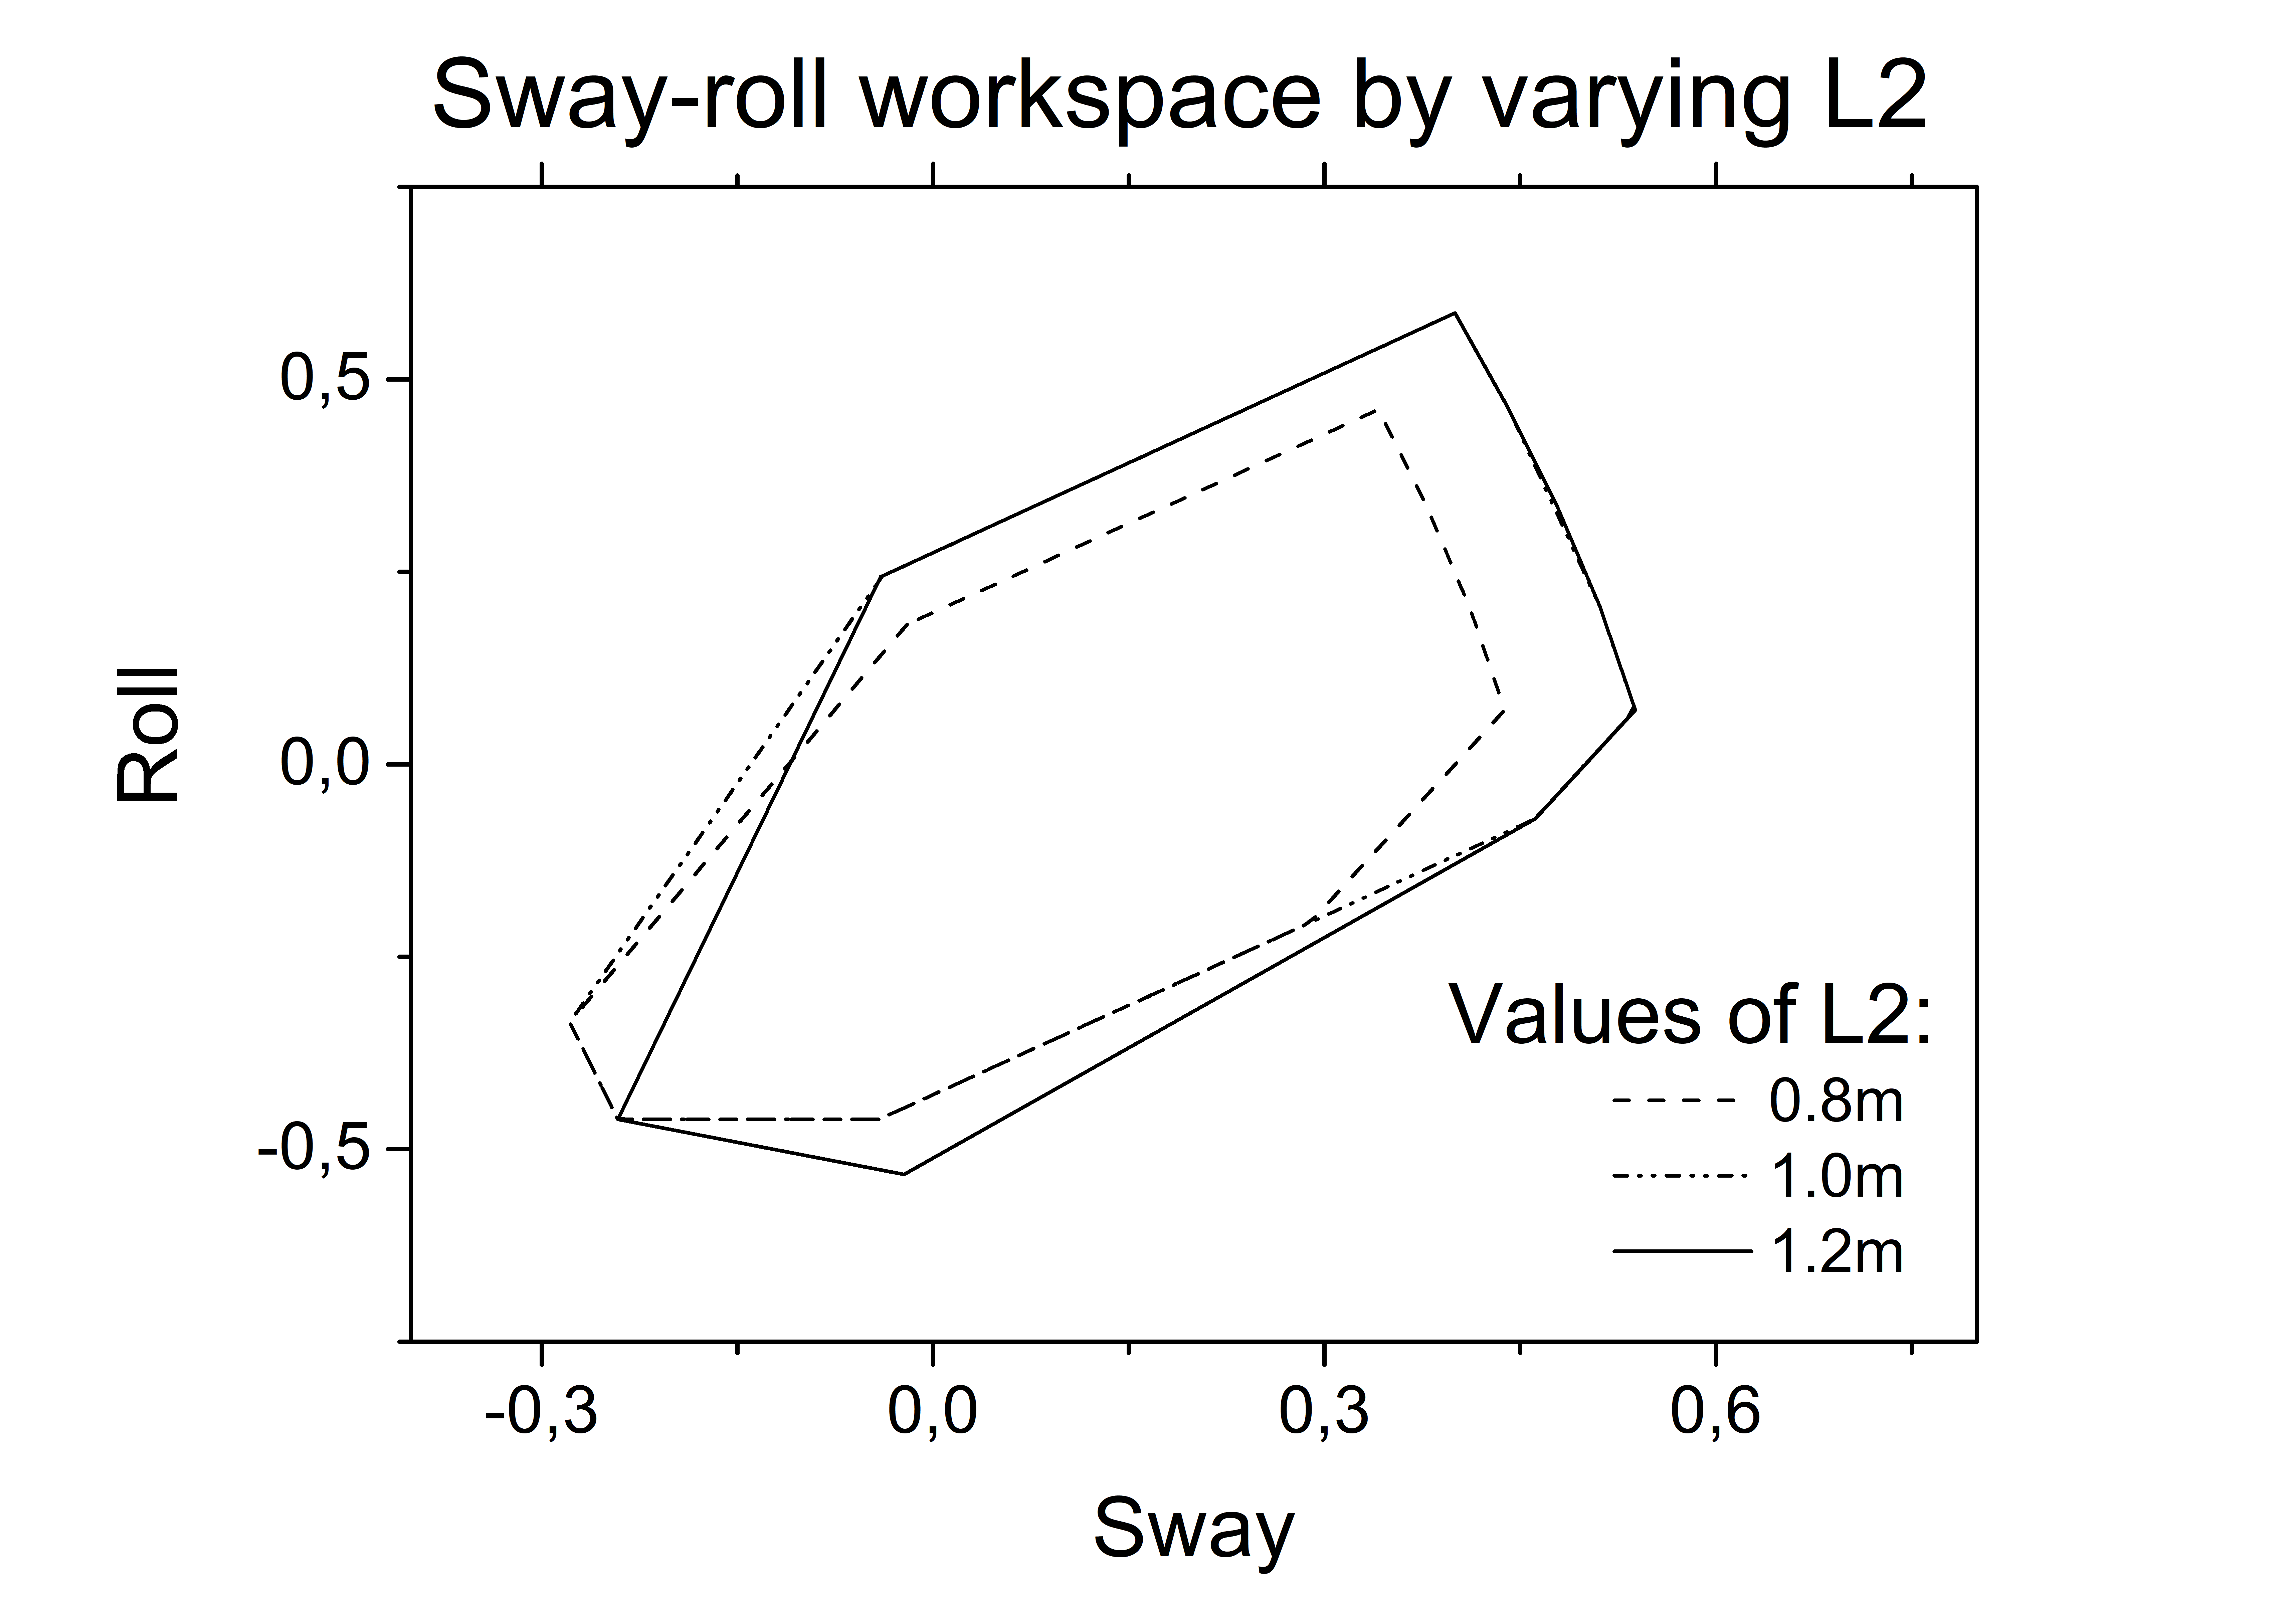
\includegraphics[width=7.5cm]{Images/ws_l2_xa}
\end{minipage}
\begin{minipage}{0.49\textwidth}
	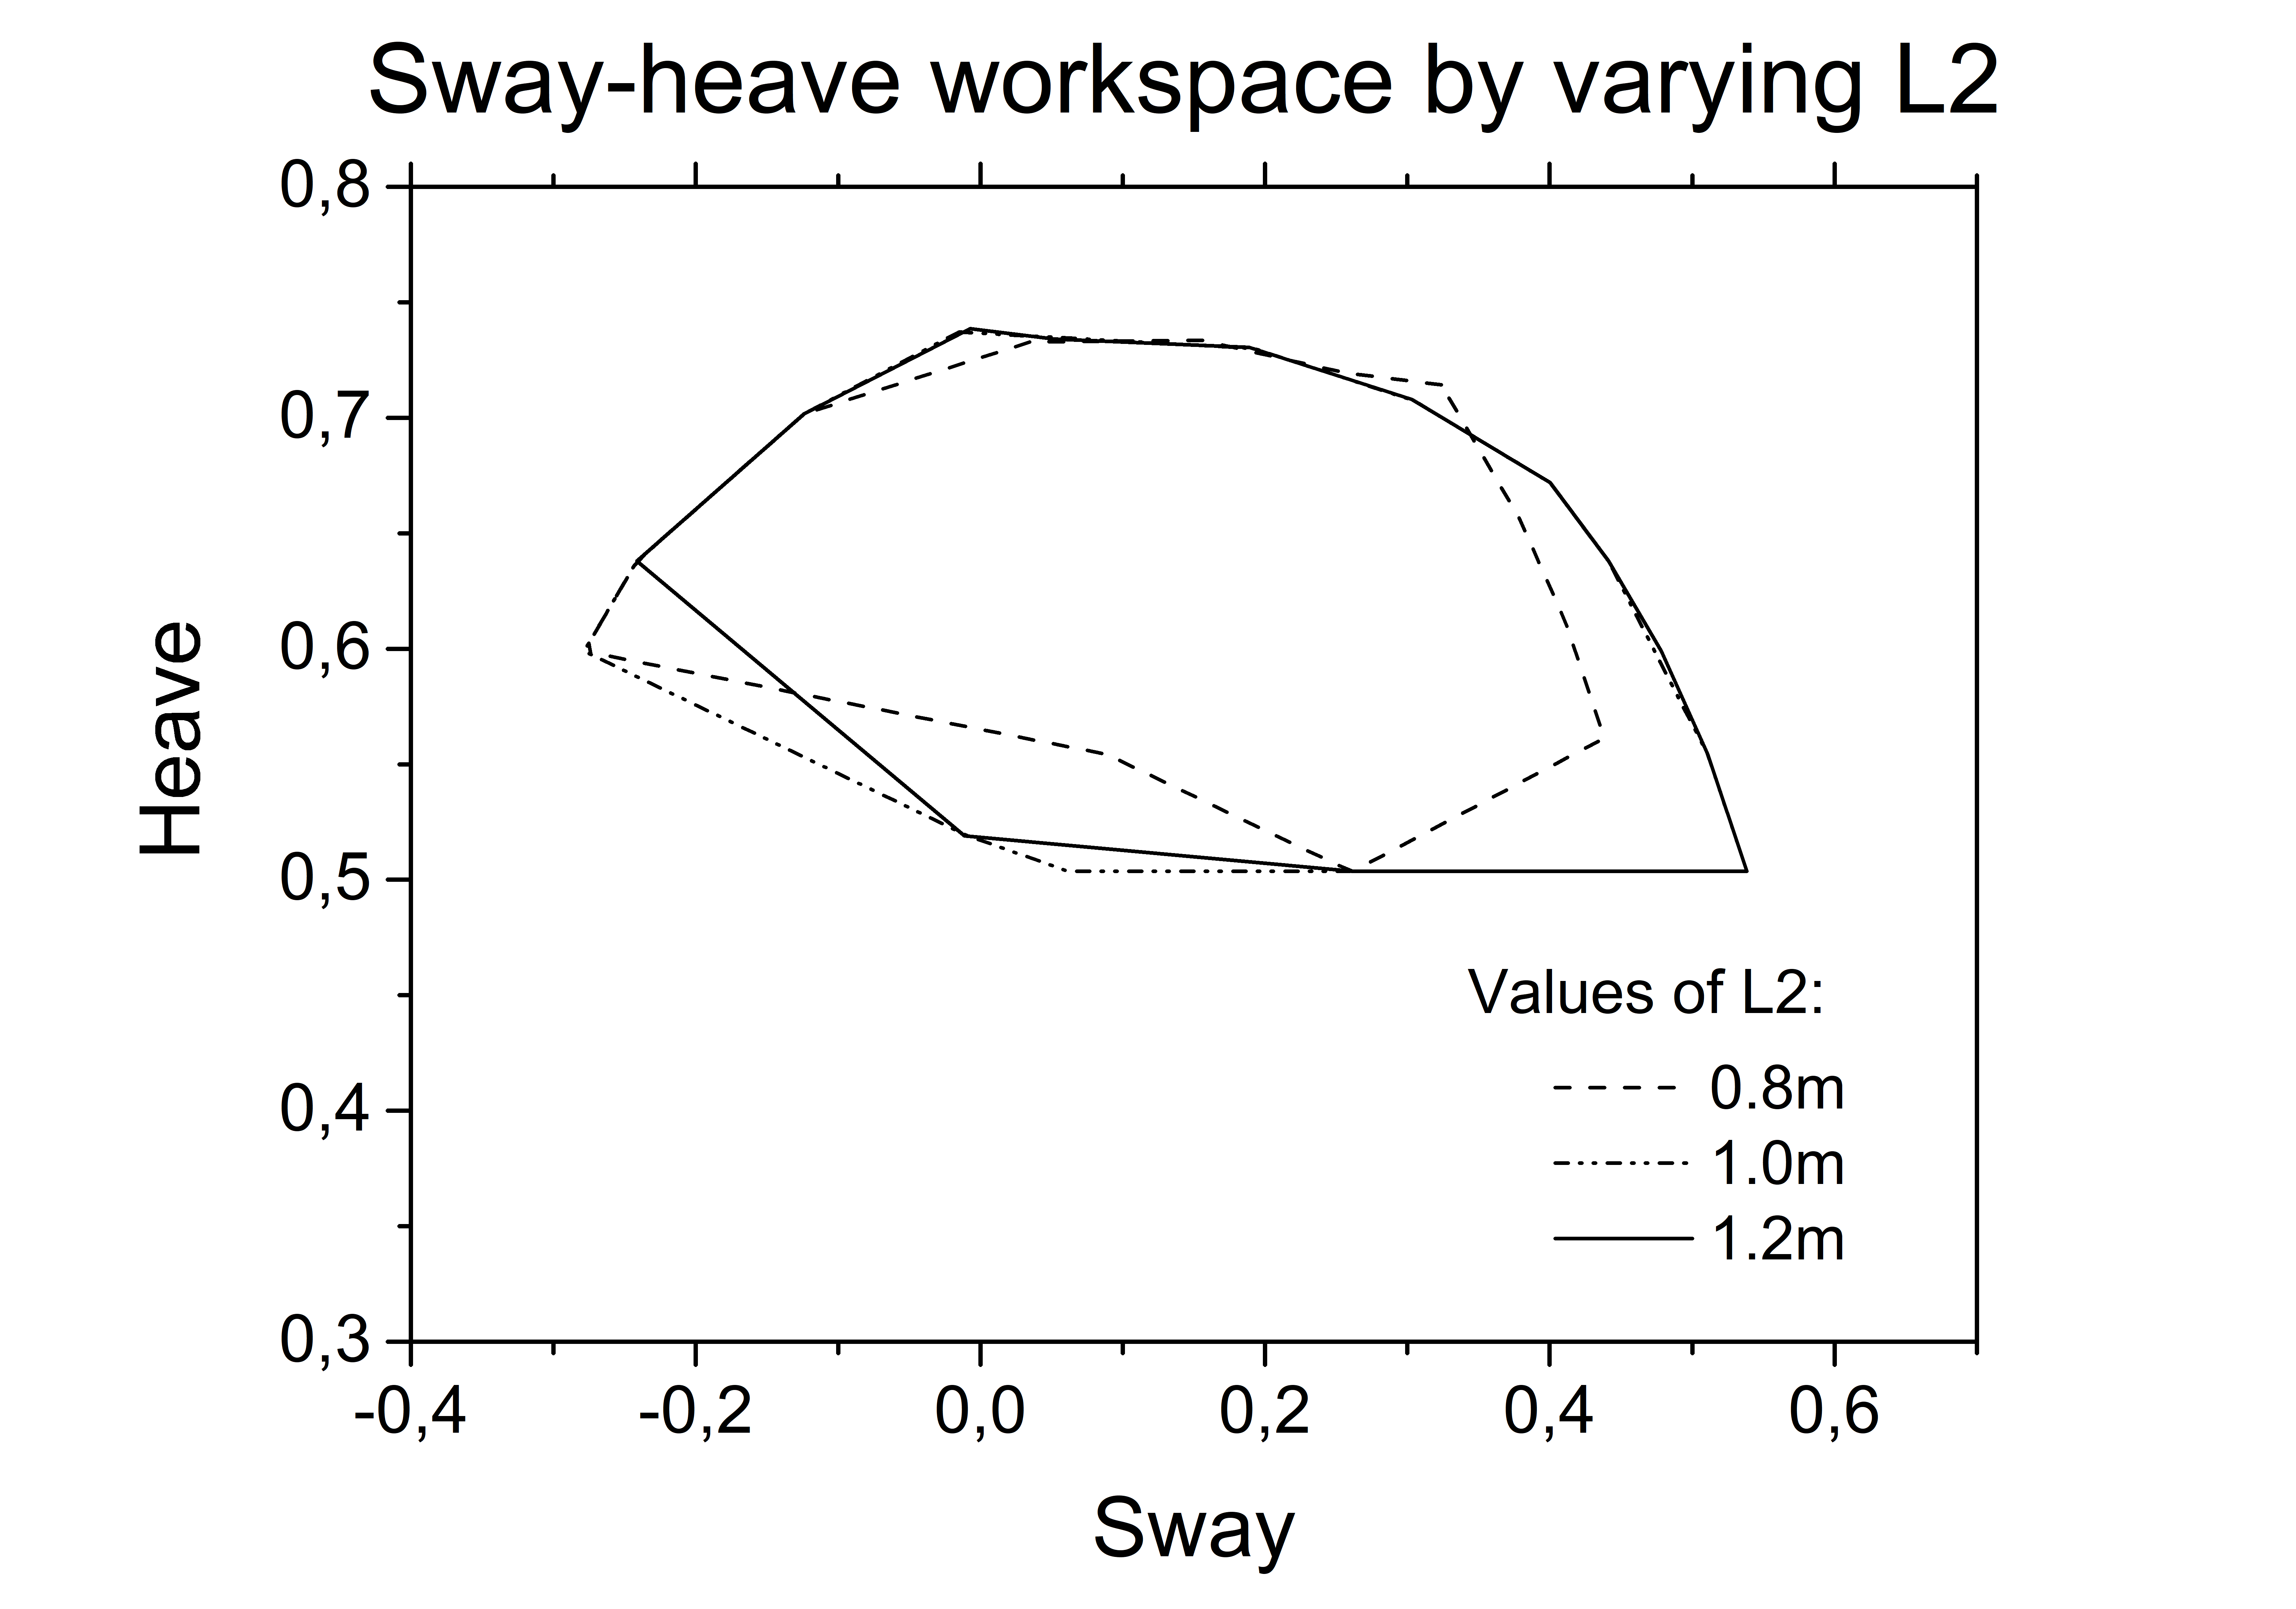
\includegraphics[width=7.5cm]{Images/ws_l2_xy}
\end{minipage}
\begin{minipage}{0.49\textwidth}
	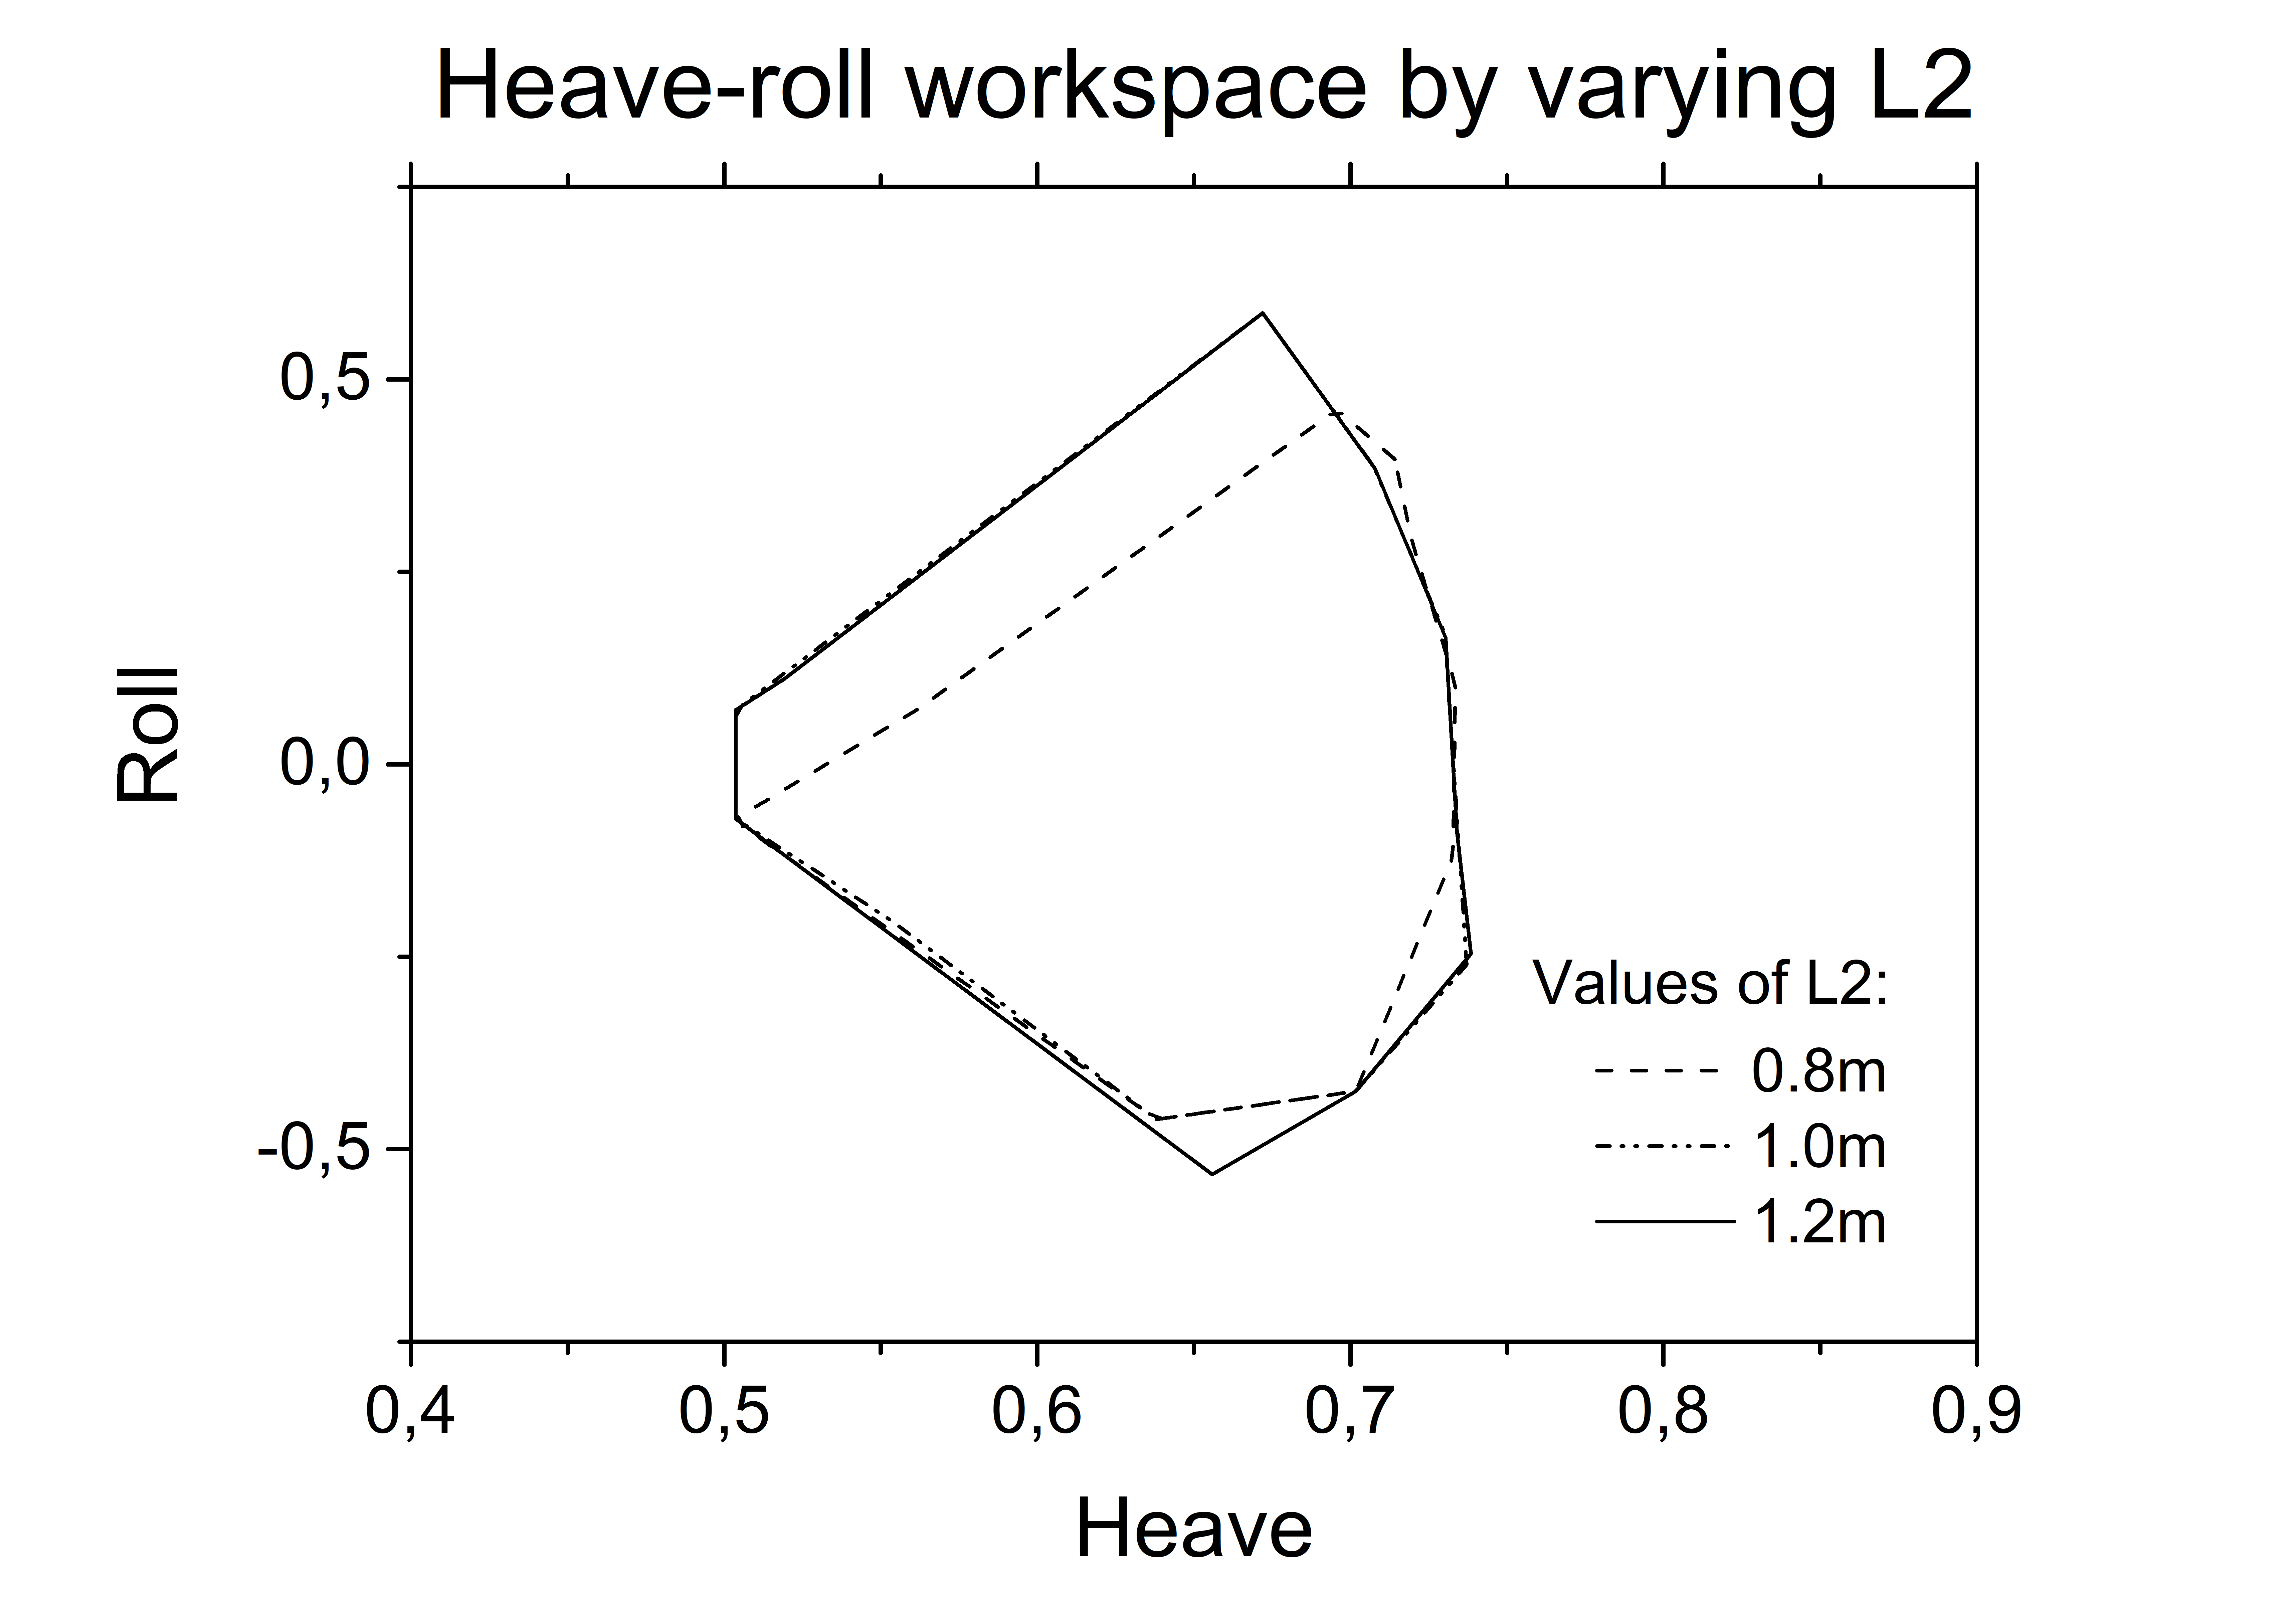
\includegraphics[width=7.5cm]{Images/ws_l2_ya}
\end{minipage}
    \caption{Variation of the workspace as a function of \( L_2 \).}
    \label{fig:ws_3}
\end{figure*}

\begin{figure*}
\centering
\begin{minipage}{0.49\textwidth}
	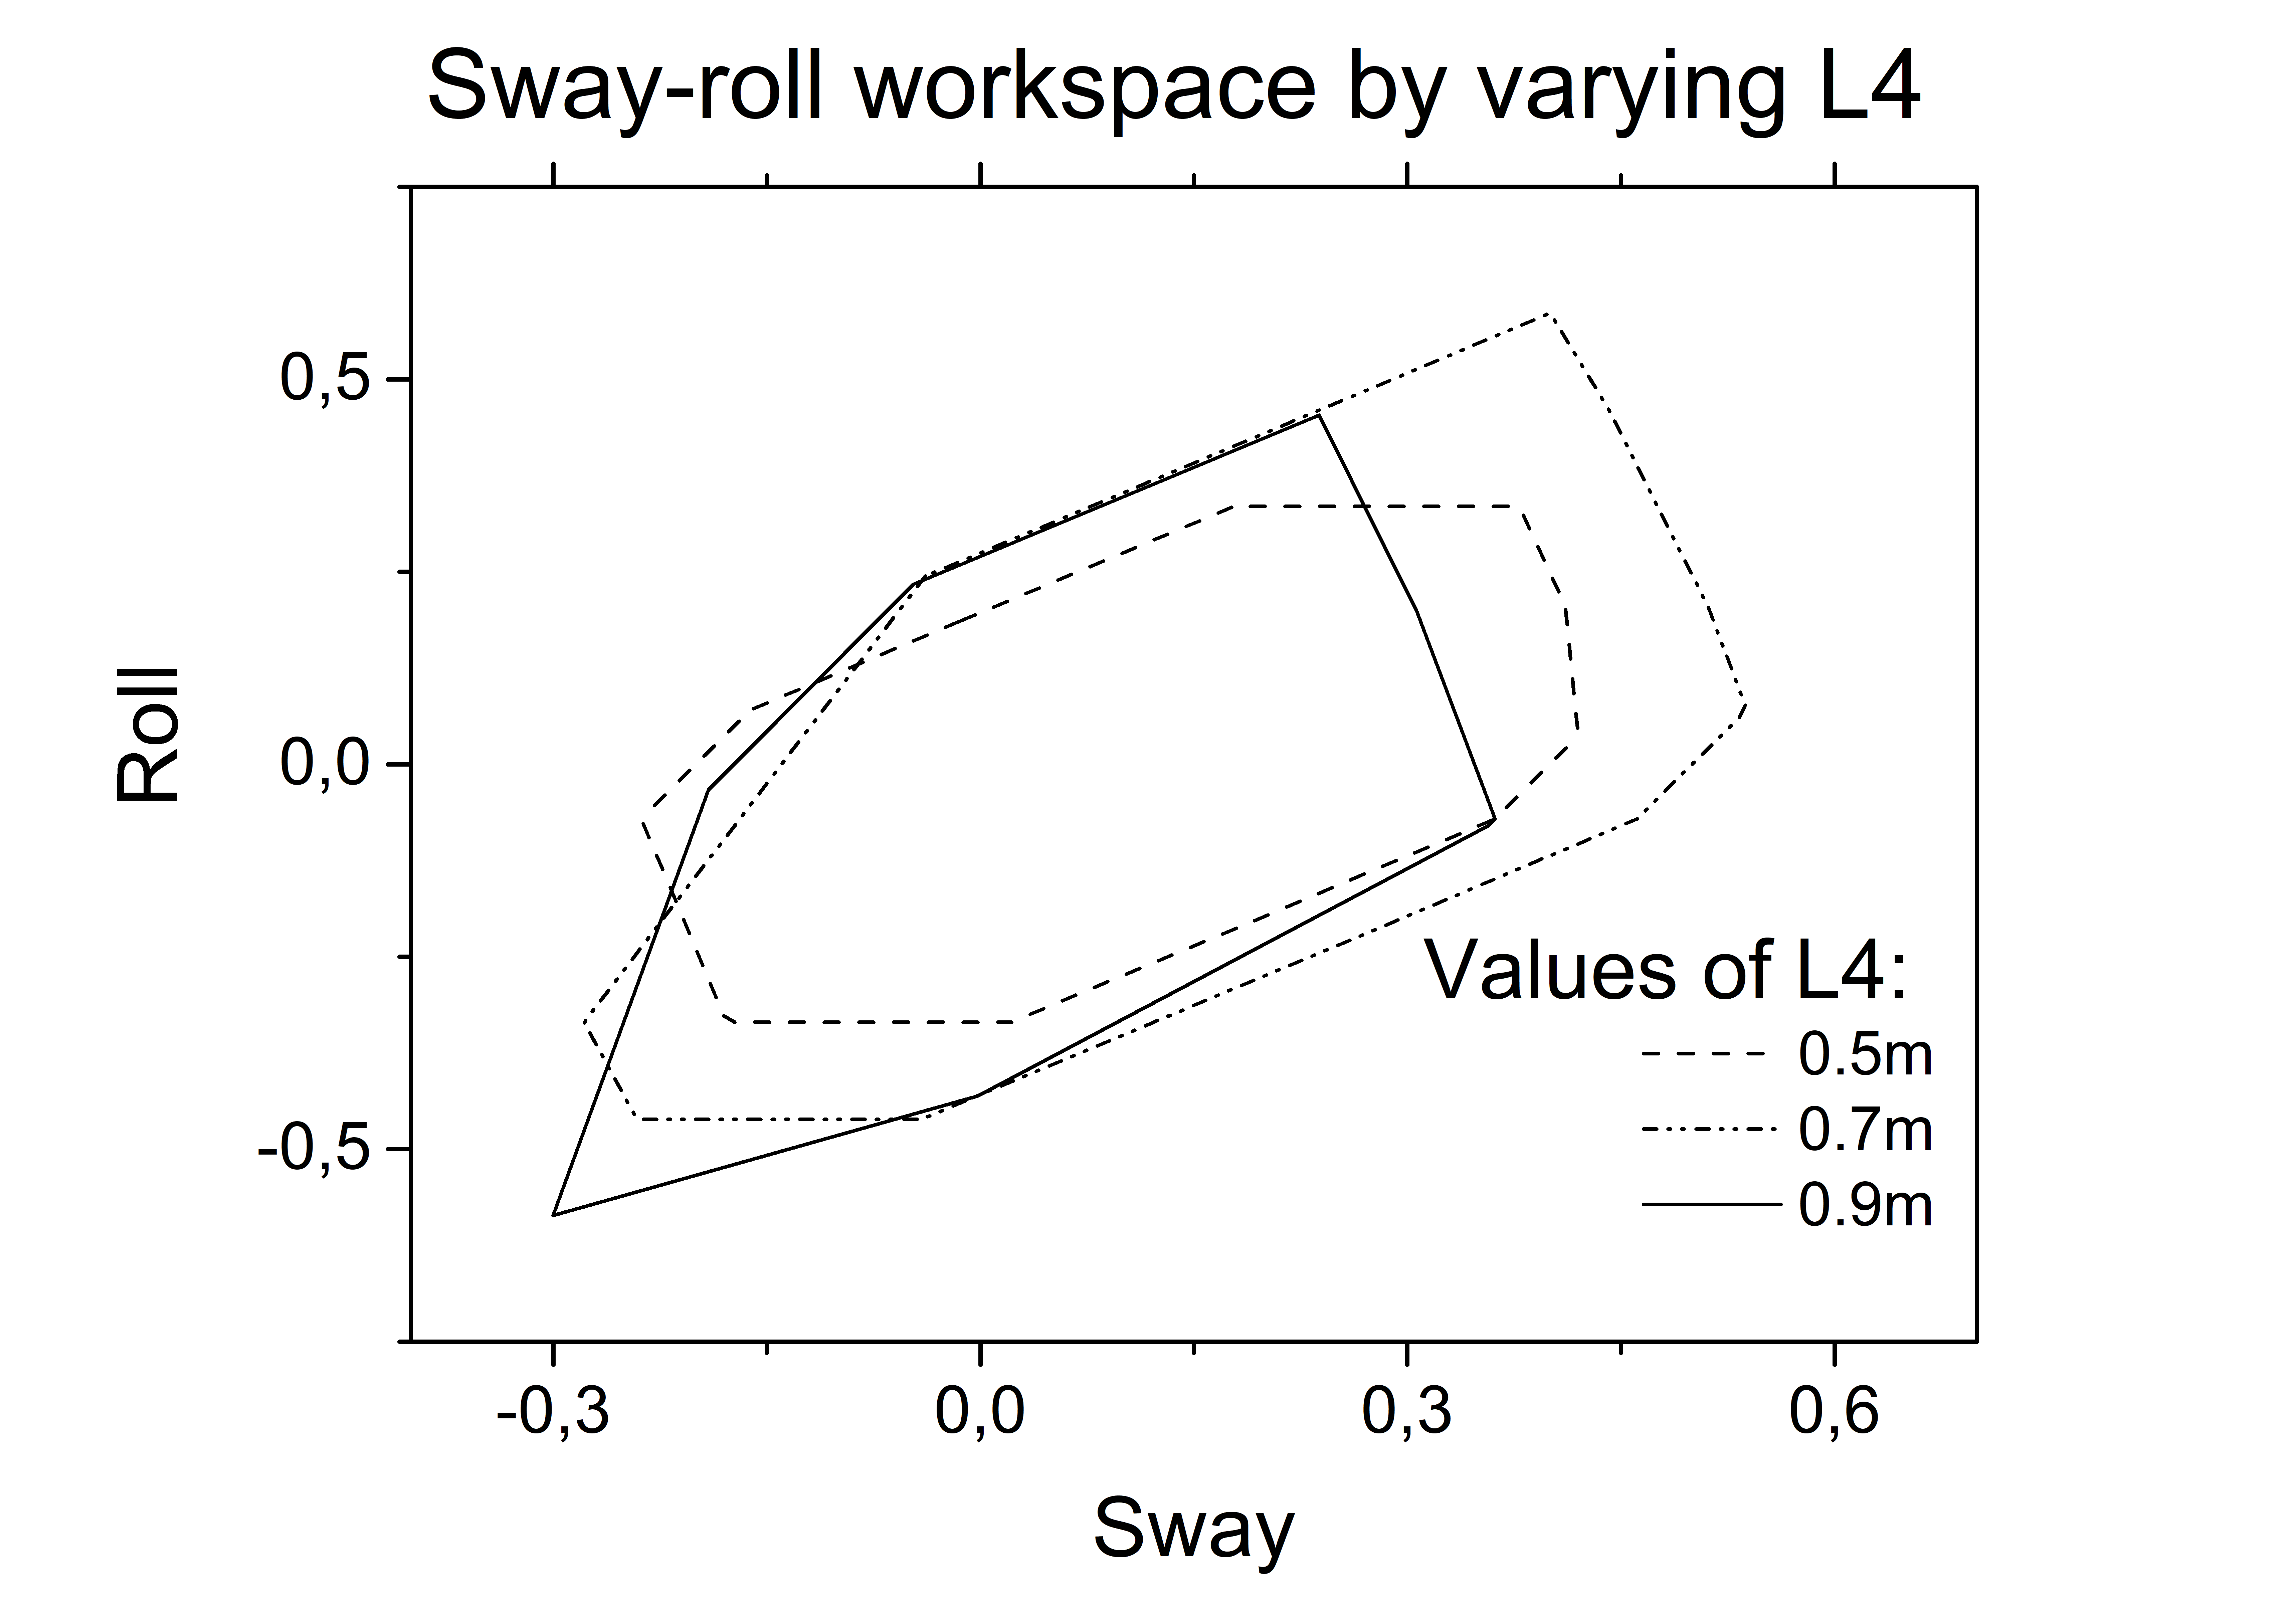
\includegraphics[width=7.5cm]{Images/ws_l4_xa}
\end{minipage}
\begin{minipage}{0.49\textwidth}
	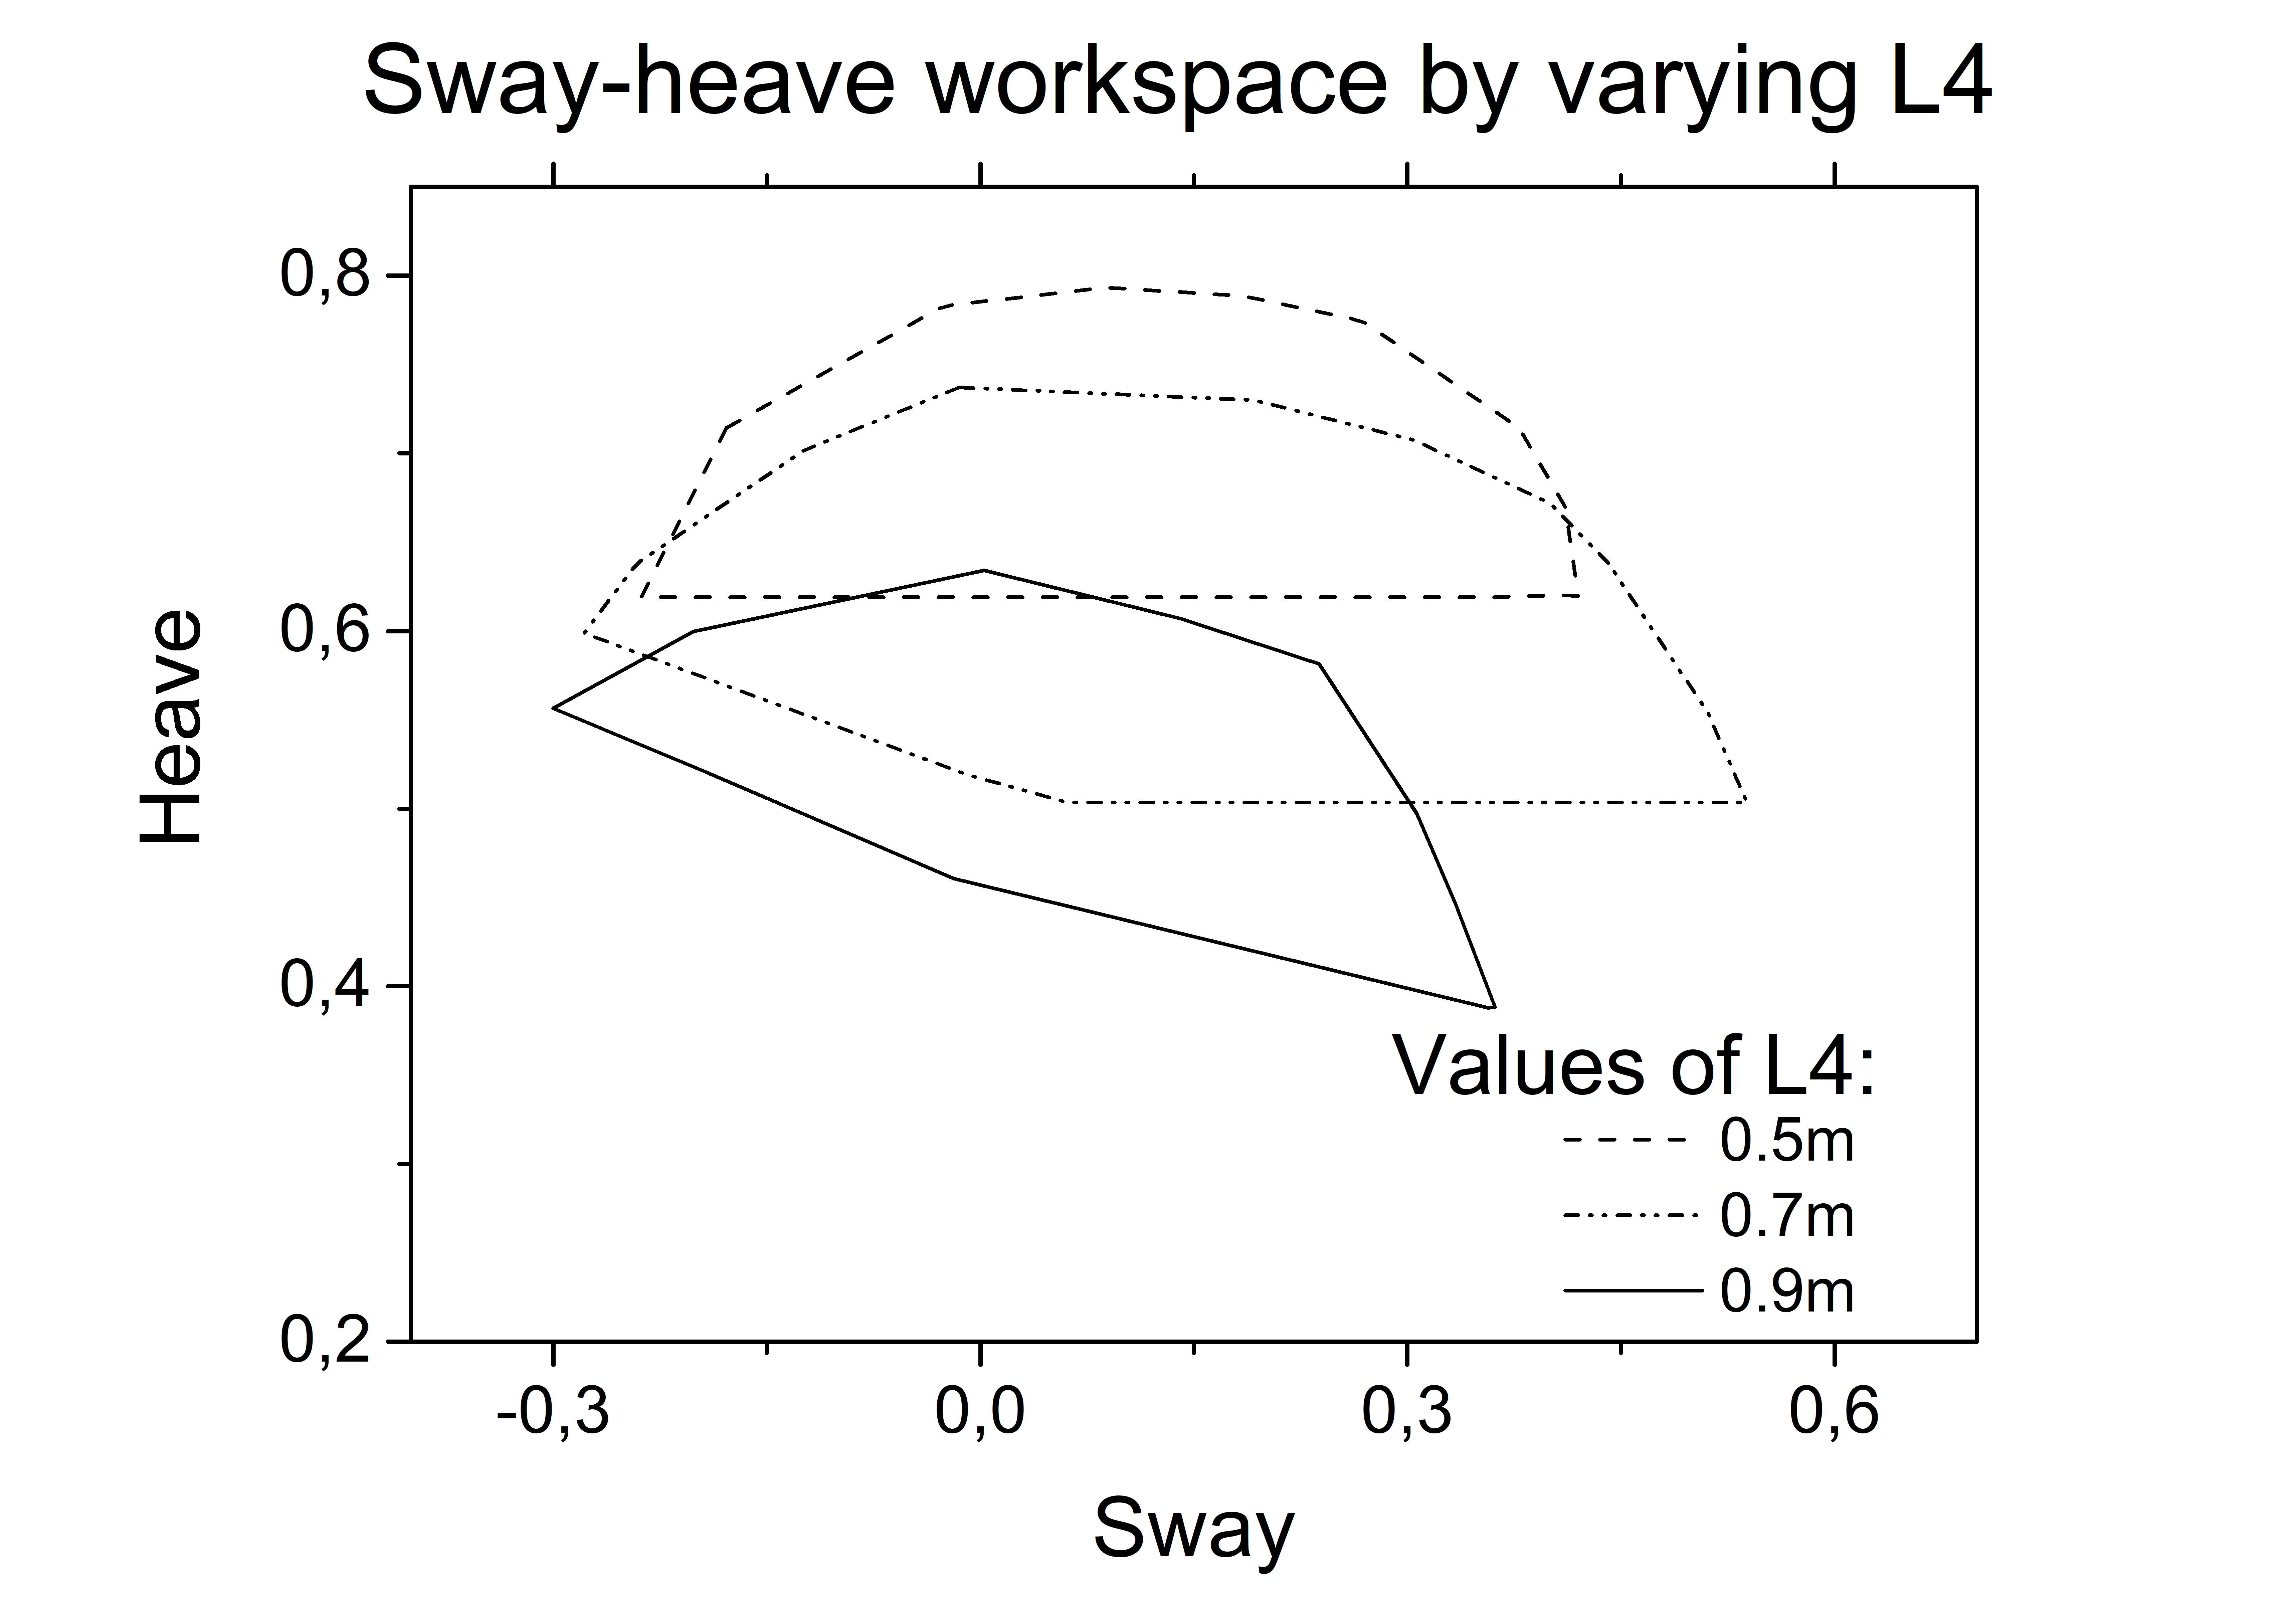
\includegraphics[width=7.5cm]{Images/ws_l4_xy}
\end{minipage}
\begin{minipage}{0.49\textwidth}
	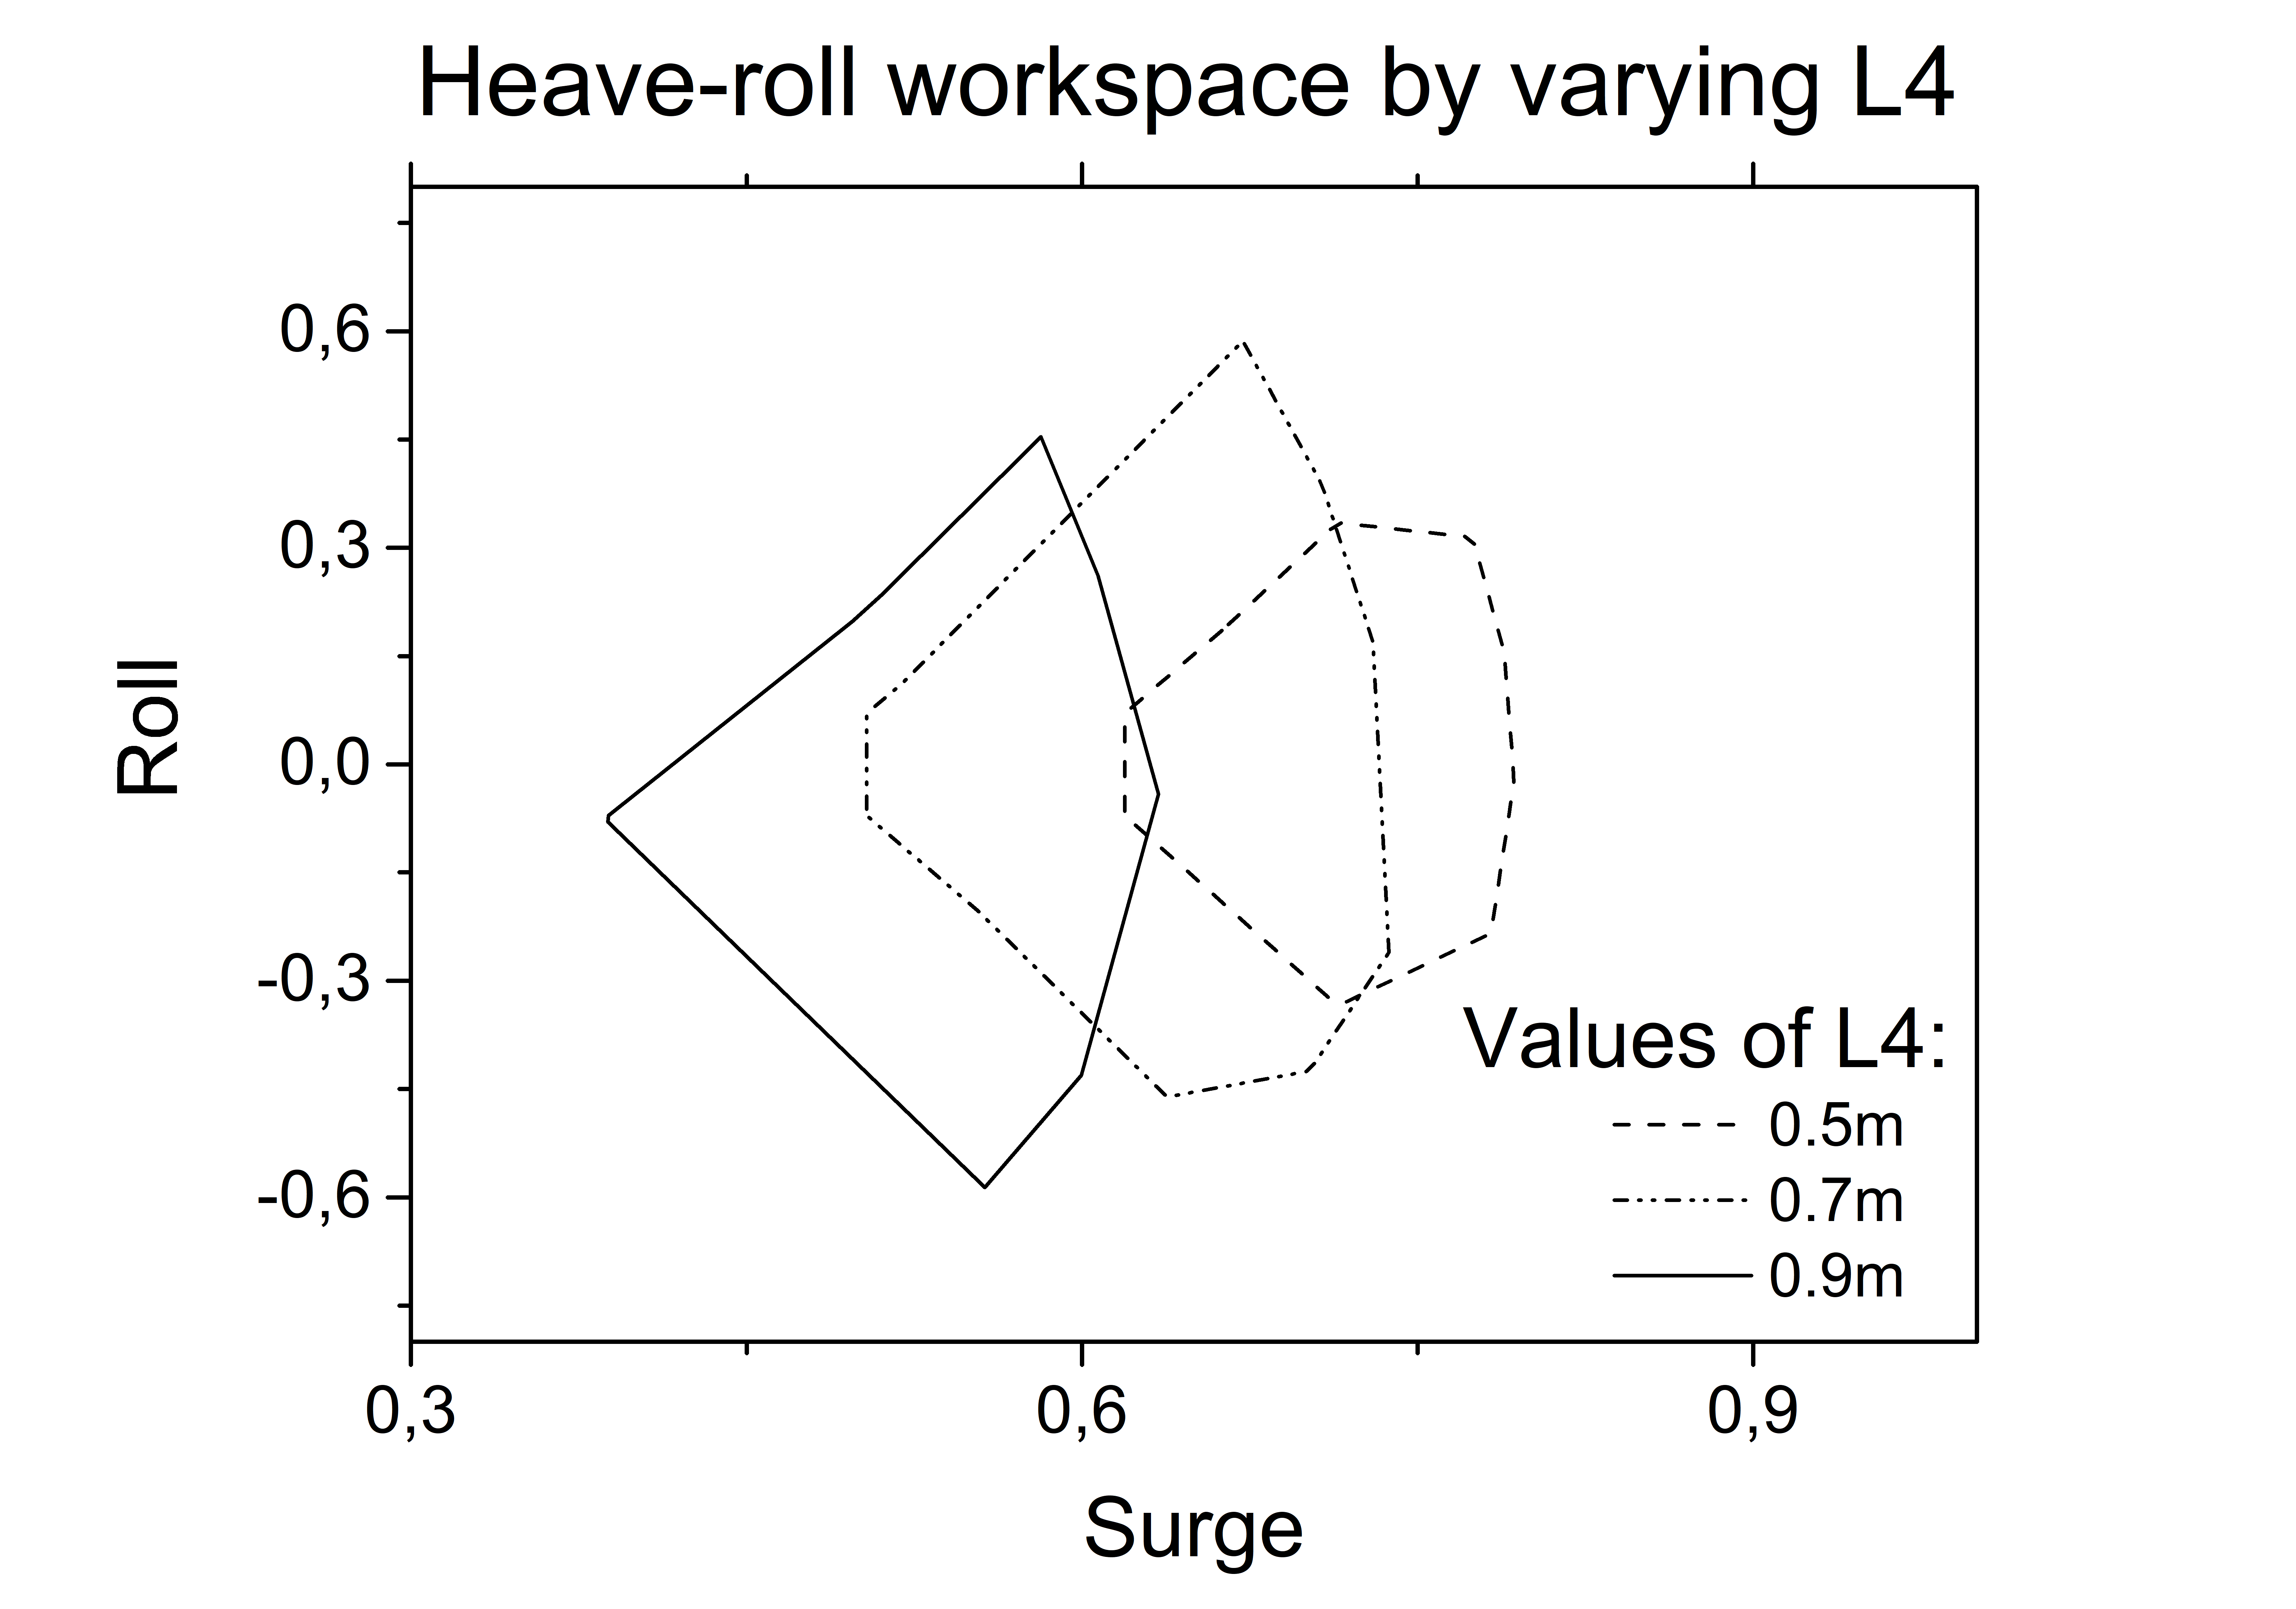
\includegraphics[width=7.5cm]{Images/ws_l4_ya}
\end{minipage}
    \caption{Variation of the workspace as a function of \( L_4 \).}
    \label{fig:ws_4}
\end{figure*}



\clearpage
\restoregeometry


\begin{thebibliography}{}
\bibitem{Biral}
Notes of the course \Virgolette{\textit{Modelling and Simulation of Mechatronic Systems}}, University of Trento, 2019.

\bibitem{aVDS}
\Virgolette{\textit{Advanced Vehicle Driving Simulator}}, \textsc{ABDynamics}.

\bibitem{CKAS}
\Virgolette{\textit{6DOF Motion System}}, \textsc{CKAS}.

\bibitem{Kasim}
M. Kasim A. J., \Virgolette{\textit{Design and development of 6-dof motion platform for vehicle driving simulator}}, Universiti Teknologi Malaysia.
\end{thebibliography}
\end{document}
